\documentclass[a4paper,12pt, oneside]{book}
\usepackage{bm}
\usepackage{siunitx}
\usepackage{cases}
\usepackage[english]{babel}
\usepackage[dvipdfmx]{graphicx}
\usepackage{subfig} 
\columnsep 3zw
\renewcommand\baselinestretch{0.8} 
\topmargin -1.5cm        % read Lamport p.163
\oddsidemargin -0.04cm  % read Lamport p.163
\evensidemargin -0.04cm  % same as oddsidemargin but for left-hand pages
\textwidth 16.59cm
\textheight 23.50cm 
% \pagestyle{empty}       % Uncomment if don't want page numbers
\parskip 7.2pt           % sets spacing between paragraphs
% \renewcommand{\baselinestretch}{1.5} 	% Uncomment for 1.5 spacing between lines
\hyphenpenalty=2000\relax
\exhyphenpenalty=2000\relax
\sloppy
\renewcommand{\baselinestretch}{1.04}
\graphicspath{{images/}}
\title{\Large Graduate School of Sciences and Technology for Innovation, Yamaguchi University\\[1cm]
Division of Fundamental Sciences\\[3cm]
\huge A Computational Model of Cell Migration of Fish Keratocytes\\[5cm]
}
\author{Yu Tokunaga}
\date{\Large \today}
\begin{document}
\pagenumbering{roman}
\maketitle
\setcounter{page}{1}
\tableofcontents
\chapter{Introduction}
\pagenumbering{arabic}
\setcounter{page}{1}
%問題提起
{\it Amoeba proteus},  a common ameba cell, migrates by stretching pseudopodia with changing its cell shape continuously.
In contrast, fish keratocytes change their shape from a circular shape to a half-moon shape when they begin migration and keep its shape during migration.
This phenomenon suggests that the deformation of the cell shape is a key feature to realize cell migration of keratocytes.

%いかに不思議か(問題点を具体化)
Actin proteins compose cytoskeleton of eukaryotic cells \cite{svitkina1997analysis}, and in keratocytes, actin molecules have been reported to extend their head toward the cell membrane by actin polymerization (AP), which has been suggested as a source of the deformation of the cell membrane and the propulsive force of the cell.
The actin retrograde flow (ARF) that pulls the actin molecules back toward the stress fiber (SF), a bundle of actin fibers spreading from side to side of the rear part of the cell, has also been reported \cite{nakashima2015molecular}.
%目的
The purpose of this research is to clarify the mechanism that forms a half-moon shape by physical simulation experiments considering intracellular mechanism.

%本稿の構成                    
The structure of this paper is as follows.
Chapter 2 introduces previous works on the molecular mechanism of cell migration of keratocytes.
Chapter 3 explains the  method of physical simulation experiments.
Chapter 4 shows the simulation results, and the last chapter concludes this study and discusses the future prospects of this study.

%第2章
\chapter{Keratocytes}
\section{Characteristics of Cell Migration of Keratocytes}
\begin{figure}[tbp]
\centering
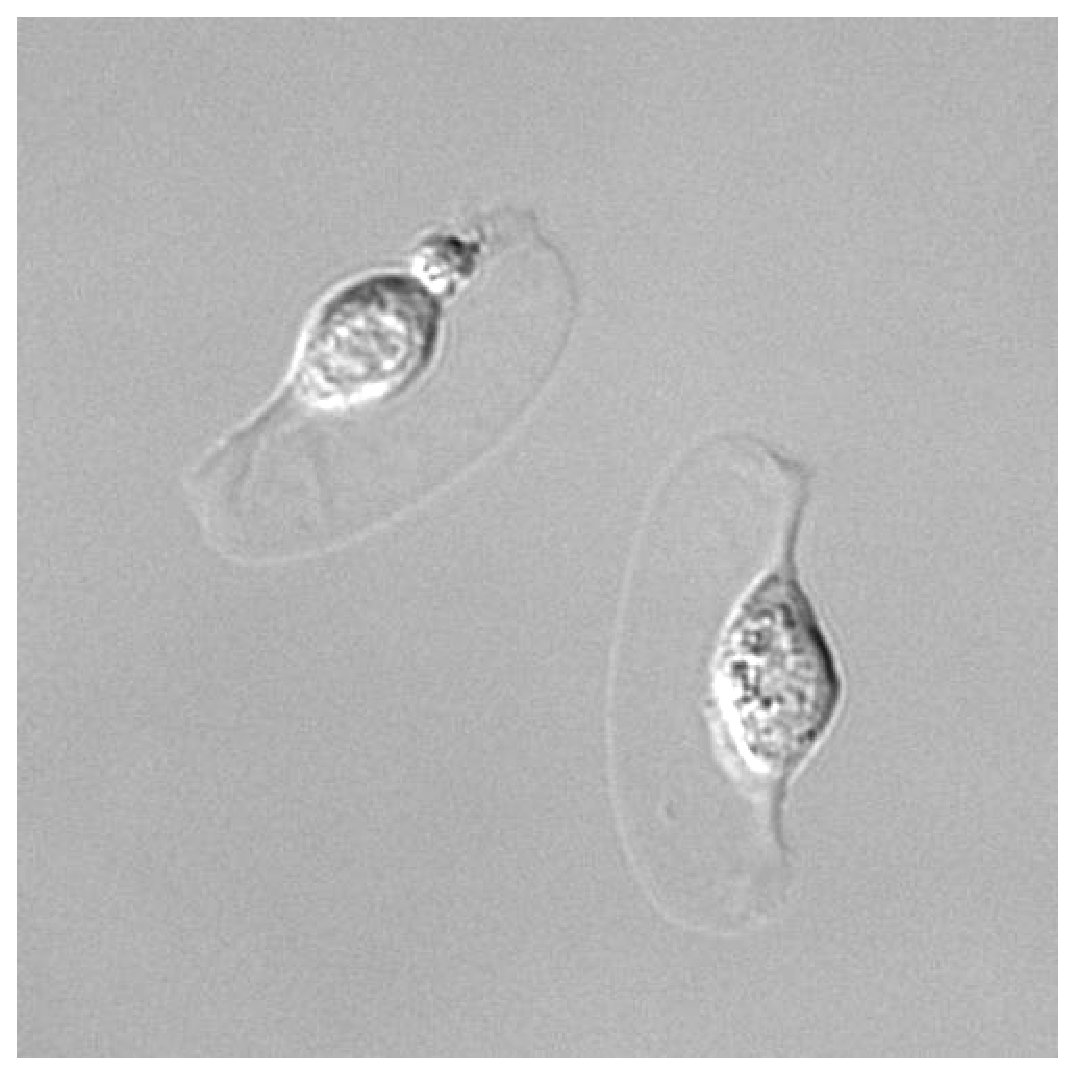
\includegraphics[scale=0.4]{kera.eps}
\caption{Keratocytes during cell migration.(Source: Takako Tanaka, Iwadate Lab).}
\label{fig:kera}
\end{figure}

%ケラトサイトの自己紹介
A keratocyte, a migratory fish epidermal cell, is a wound healing cell about \SI{70}{\mu m}  in size.
When a fish is injured, keratocytes begin migration toward the injured position toward  the wound by the speed of about one body length in one minute.
The locomotion of keratocytes is a kind of amoeboid movements;
however, it is different from typical amoeba movement at the point that they move with keeping a half-moon shape. 

%参考文献
%アクチン分子
The cell migration of keratocytes has been suggested to be caused by actin polymerization (AP)\cite{svitkina1997analysis}.
AP is a phenomenon in which cytoskeletal actin molecules linearly bind to form filamentous actin (F-actin).
%cell migration と actinの重合と脱重合の関連
The AP occurs only at one end of F-actin, depolymerization occurs at the opposite end.
The polymerized actin molecules form a dense network and push the cell membrane from the inside.
It has been reported that the actin molecules are polymerized more frequently in higher density regions of actin molecules and depolymerized less in lower density regions \cite{yumura1998spatiotemporal}.
%ARFとSFの紹介
There is a stress fiber (SF) at the rear of the cell.
The SF is a bundle of actomyosin composed of actin molecules and myosin molecules.
The actin retrograde flow (ARF) which pulls the actin molecules back toward the SF has also been reported \cite{swaminathan2017actin}.
%cell migrationとARFとSFの関連
Other study have reported that the ARF  orient the actin molecules towards the SF\cite{nakata2016role}.
When SF is removed, the shape of the cell collapses and the moving speed slows down.
This also indicates the importance of SF for cell migration.
Okimura et al. reported that the SF plays the role of wheels in cell migration \cite{okimura2018rotation}.
It has been reported that the formation of a half-moon shape at the time of migration was observed even after removal of the nucleus \cite{asano2004keratocyte}.
These reports suggest that for the cell migration of keratinocytes, not the nuclear part but the other parts where SF and F-actin exist are important.

\section{Molecular Mechanism of Cell Migration}
A cell has a structure called a cytoskeleton.
The cytoskeleton is like bones of humans and forms a cell shape, however, it shows dynamic behavior  in contrast to the rigid nature of human bones.
One of the  main components of the cytoskeleton is actin molecules.
The polymerization and depolymerization of actin molecules change the cell shape.
The actin molecule extends toward the cell membrane by polymerization and is attracted to the SF by the ARF.
The membrane of amoeboid cells is extruded by the polymerization of actin molecules and forms pseudopodia which adhere to the substrate under the pseudopodia.
Thereafter, the adhesion to the substrates of the rear part of the cell is released and the cell is dragged forward.
By repeating this cycle, cell migration is realized.
The cell membrane of keratocytes is also deformed by actin molecule polymerization.
By the simulation experiment described in the next chapter, we investigate how the cell membrane forms a half-moon shape by the actin molecule polymerization. 
\chapter{Simulation Methods}
\section{Simulation Methods of Cell Membrane}
%初期配置の話
In the computer simulation of this study, the cell membrane was modeled by a network of simple particles interacting with each other and placed on a cylindrical surface as an initial condition.
Each particle of the membrane was assumed to receive elastic force from neighboring particles and repulsive force from actin molecules.
The equation of motion of the cell membrane molecule was assumed as follows.

\begin{equation}
m\frac{d^2\bm{x}_i}{dt^2} = \bm{F}^m_i +  \bm{F}^a_i - \eta \frac{d\bm{x}_i}{dt}
\end{equation}

where  $\bm{x}_i$ is the position vector of the membrane molecule, $m$ is the mass of the particle, $\eta=8.9\times10^{-6}\si{~kg/s}$ is the viscous coefficient, $\bm{F}^m_i$ and $\bm{F}^a_i$ are the forces received from the neighboring particles and  the repulsive force from actin molecules.
The force  $\bm{F}^m_i$ was assumed as an elastic force:
\begin{equation}
\bm{F}^m_i = \sum_{i \in I_j}  -k((\bm{x}_j -\bm{x}_i )-\bm{l}_{ij} )
\end{equation}
where $k$ is a spring constant, $\bm{l}_{ij}$ is the natural length between the $i$-th and $j$-th membrane particles, and $I_j$ represents the set of particles that interact with particle $j$.
The natural length between particles was determined by the distance  at the initial state.
The force $\bm{F}^a_i$ received from an actin particle was assumed to be a  repulsive force:
\begin{equation}
\bm{F}^a_i = \sum_{\{ \forall i | \| \bm{x}_j - \bm{B}_i \|<D_2\}} \frac{s}{\|\bm{x}_j -\bm{B}_i \|} \frac{\bm{x}_j -\bm{B}_i }{\|\bm{x}_j -\bm{B}_i \|}
\end{equation}
where $s$ is a constant that determines the strength of the repulsive force, and $D_2$ is a distance range of the effect of the force prepared to decrease the calculation amount.

\section{Simulation Methods of Actin Molecules}
\subsection{Actin Polymerization}
An actin molecule has polarity: one end which elongates by the polymerization is called barbed-end, and the other end is called pointed-end.
Since the frequency of polymerization is high in a region where actin molecules are dense \cite{yumura1998spatiotemporal}, the polymerization rate was assumed to be  proportional to the actin concentration.
The filament formed by actin polymerization is called F-actin.
F-actin was expressed by a simple  rod in the simulation. 
As an initial condition,  the length of each rod was zero and the direction of the actin polymerization $\bm{L}_i$ was  randomly determined.
The elongation of the F-actin by the polymerization is modeled by
\begin{equation}
\bm{B}_i \gets \bm{P}_i + f^p(c)\bm{L}_i \cdot dt
\end{equation}
where $\bm{B}_i$ and $\bm{P}_i$ are the barbed end and pointed end of the F-actin, respectively, and $f^p(c) = 5.0~\exp{\frac{c}{10.0}}$ expresses the frequency of actin polymerization as a function of actin concentration $c$ which was computed for each region by dividing the simulation space into a grid.
The frequency of depolymerization decreases in an actin dense area and the depolymerization was expressed  as follows.
\begin{equation}
\bm{P}_i \gets \bm{P}_i + f^d(c)\bm{L}_i \cdot dt
\end{equation}
where $f^d(c) = \frac{5.0}{c}$ represents the frequency of depolymerization. 
The actin polymerization and depolymerization was simulated by a probability  \[p_i(c) = c_i = \frac{a_i}{N}\] at each step, where $p_i(c)$ is the probability that depends on the concentration $c_i$ in $i$-th region, $a_i$ is the number of actin in $i$-th region, and $N$ is the total number of actin.
In this simulation, the simulation space was divided into $225$ regions $(i = 1,...225$).

The actin molecules in the region with a low density of actin molecules were assumed to disappear and the same number of new actin molecules were put near the cell membrane.
The direction of polymerization of each actin was randomly determined at the initial state. 
In this experiment, the disappearance condition of the actin molecule is $c_i<0.06$.

\subsection{Actin Retrograde Flow}
The ARF is a movement of F-actins toward the stress fiber which is a bundle of actin fibers aligning from side to side in the rear side of a keratocyte. 

We assumed the ARF as the retraction of the actin molecules toward the leftmost point of the cell in Fig.\ref{fig:ini}, i.e., the position of the membrane particle with the smallest $x$ coordinate which we call the reference point. The retraction of the actin molecules by the ARF was expressed by the following equation:
\begin{numcases}
  {}
  \bm{B}_i \gets \bm{B}_i - \alpha \frac{ \bm{B}_i - \bm{E}_0}{{\| \bm{B}_i - \bm{E}_0 \|}^w}\cdot dt & \\
   \bm{P}_i \gets \bm{P}_i - \beta \frac{ \bm{P}_i - \bm{E}_0}{{\| \bm{P}_i - \bm{E}_0 \|}^w}\cdot dt  &
   \label{eq:arf1}
\end{numcases}
where $\bm{E}_0$ is the reference point, and $\alpha$ and $\beta$ are constants that determine the strength of the ARF.
$w$ is a parameter indicating the effect of distance between the actin molecule and cell membrane molecule on the retraction strength of the ARF.
When $w=2$, the closer the intermolecular distance is, the stronger the retraction is.
When $w=1$, all actin molecules are equally pulled irrespective of the intermolecular distance.
When $\alpha=\beta$, the orientation effect is ineffective, therefore, the actin molecule is retracted without changing the direction.

\begin{figure}[tbp]
\centering
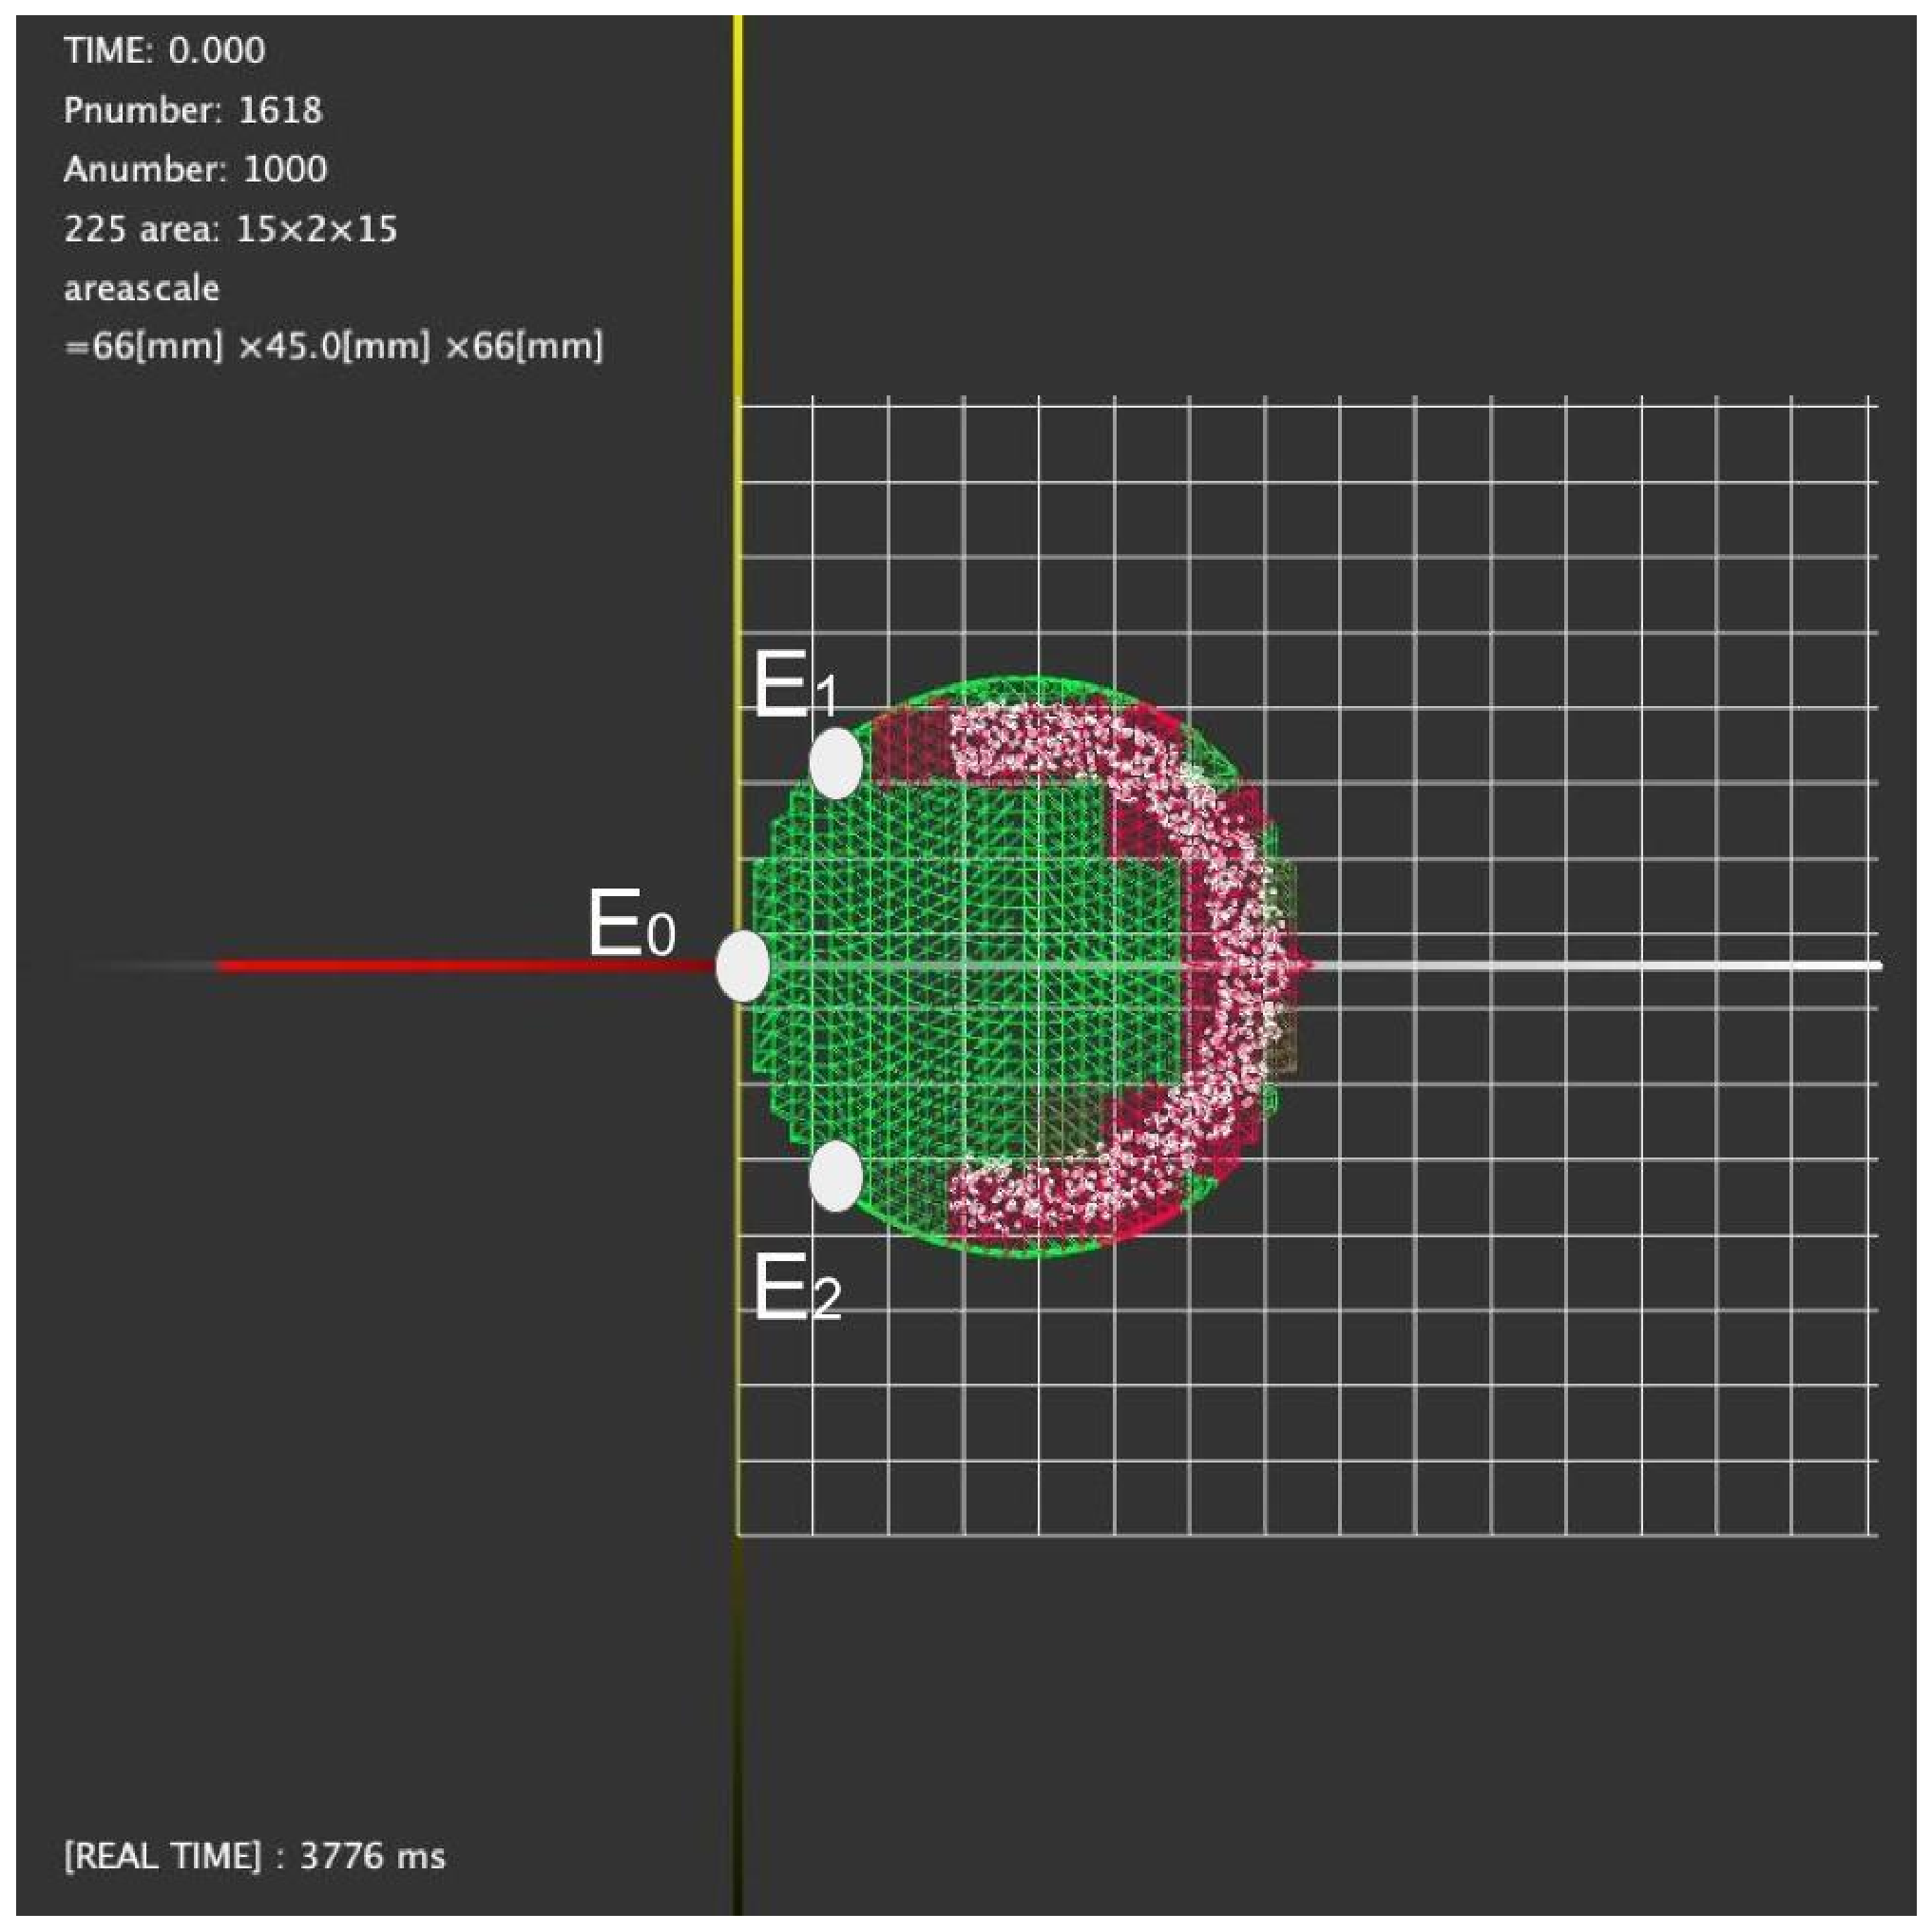
\includegraphics[width=6cm]{ind.eps}
\caption{Location of the ARF reference point, $\bm{E}_0$, $\bm{E}_1$ and $\bm{E}_2$.}
\label{fig:ind}
\end{figure}

We also investigated the case that two reference points $\bm{E}_1$ and $\bm{E}_2$ are prepared in order to express the retraction of actin molecules toward the SF.
In this case, assuming that SF spreads linearly at a distance of 1/5 from the left end of the cell (Fig. \ref{fig:ind}) and the reference points $\bm{E}_1$ and $\bm{E}_2$ were put at both ends.
The ARF was expressed by the retraction of actin molecules toward the direction of the sum of vectors from the actin molecules to the reference points:

\begin{numcases}
  {}
  \bm{B}_i \gets \bm{B}_i - \gamma \left( \frac{ \bm{B}_i - \bm{E}_1 }{{\| \bm{B}_i - \bm{E}_1 \|}^w} + \frac{ \bm{B}_i - \bm{E}_2}{{\| \bm{B}_i - \bm{E}_2 \|}^w} \right)\cdot dt & \\
   \bm{P}_i \gets \bm{P}_i - \delta \left( \frac{ \bm{P}_i - \bm{E}_1 }{{\| \bm{P}_i - \bm{E}_1 \|}^w} + \frac{ \bm{P}_i - \bm{E}_2}{{\| \bm{P}_i - \bm{E}_2 \|}^w}  \right)\cdot dt  &
   \label{eq:arf}
\end{numcases}
where $\gamma$ and $\delta$ are constants that determine the strength of the ARF.
As in eq. \ref{eq:arf1}, the orientation effect of ARF can be controlled by the magnitude relation of $\gamma$ and $\delta$.
Table \ref{ta:pra} shows the values of $\alpha, \beta, \gamma$ and $\delta$.

\begin{table}[htb]
\centering
\caption{The value of each parameter.}
\label{ta:pra}
  \begin{tabular}{|c|c|c|c|c|} \hline
  & $w=1$ & $w=2$  & 
  \begin{tabular}{c} 
  $w=1$ \\(No orientation) 
  \end{tabular}
  & 
    \begin{tabular}{c} 
  $w=2$\\(No orientation)
    \end{tabular} \\ \hline
  $\alpha$ & 5.0 & 0.02 & 20.0& 0.1  \\
    $\beta$ & 50.0 & 0.2 & 20.0 & 0.1  \\
      $\gamma$ & 2.5 & 0.01 & 10.0 & 0.05  \\
        $\delta$ & 25.0 & 0.1 & 10.0 & 0.05  \\ \hline
          \end{tabular}
\end{table}

\section{Initial Condition}
\begin{figure}[tbp]
\centering
 \subfloat[]{%
  \begin{tabular}{c}
   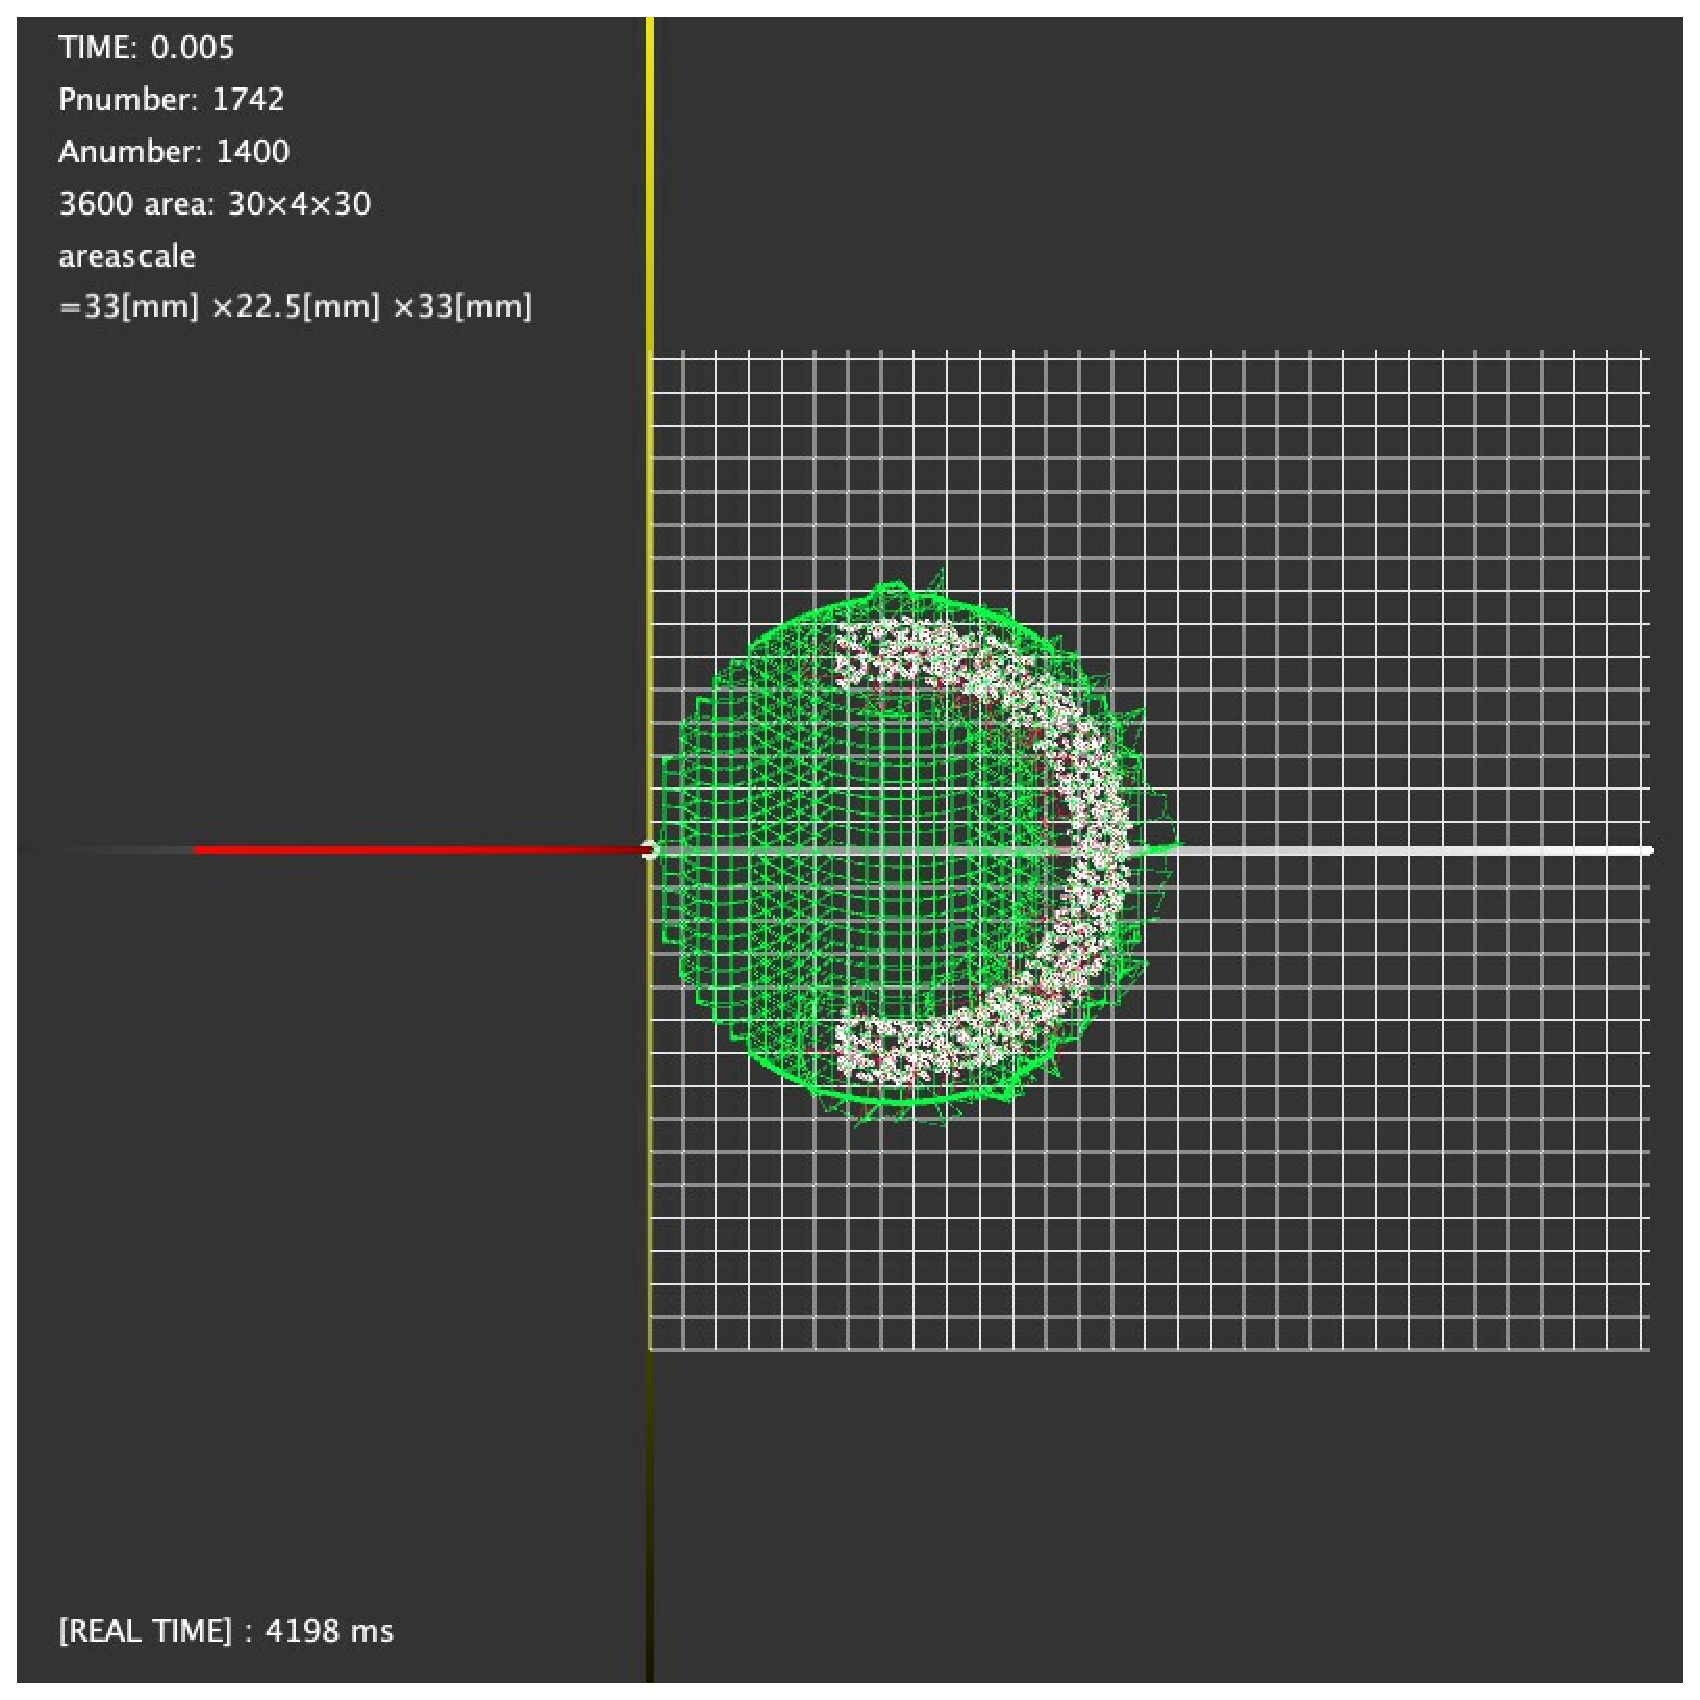
\includegraphics[width=5cm]{top.eps} 
  \end{tabular}
 }%
 \subfloat[]{%
  \begin{tabular}{c}
   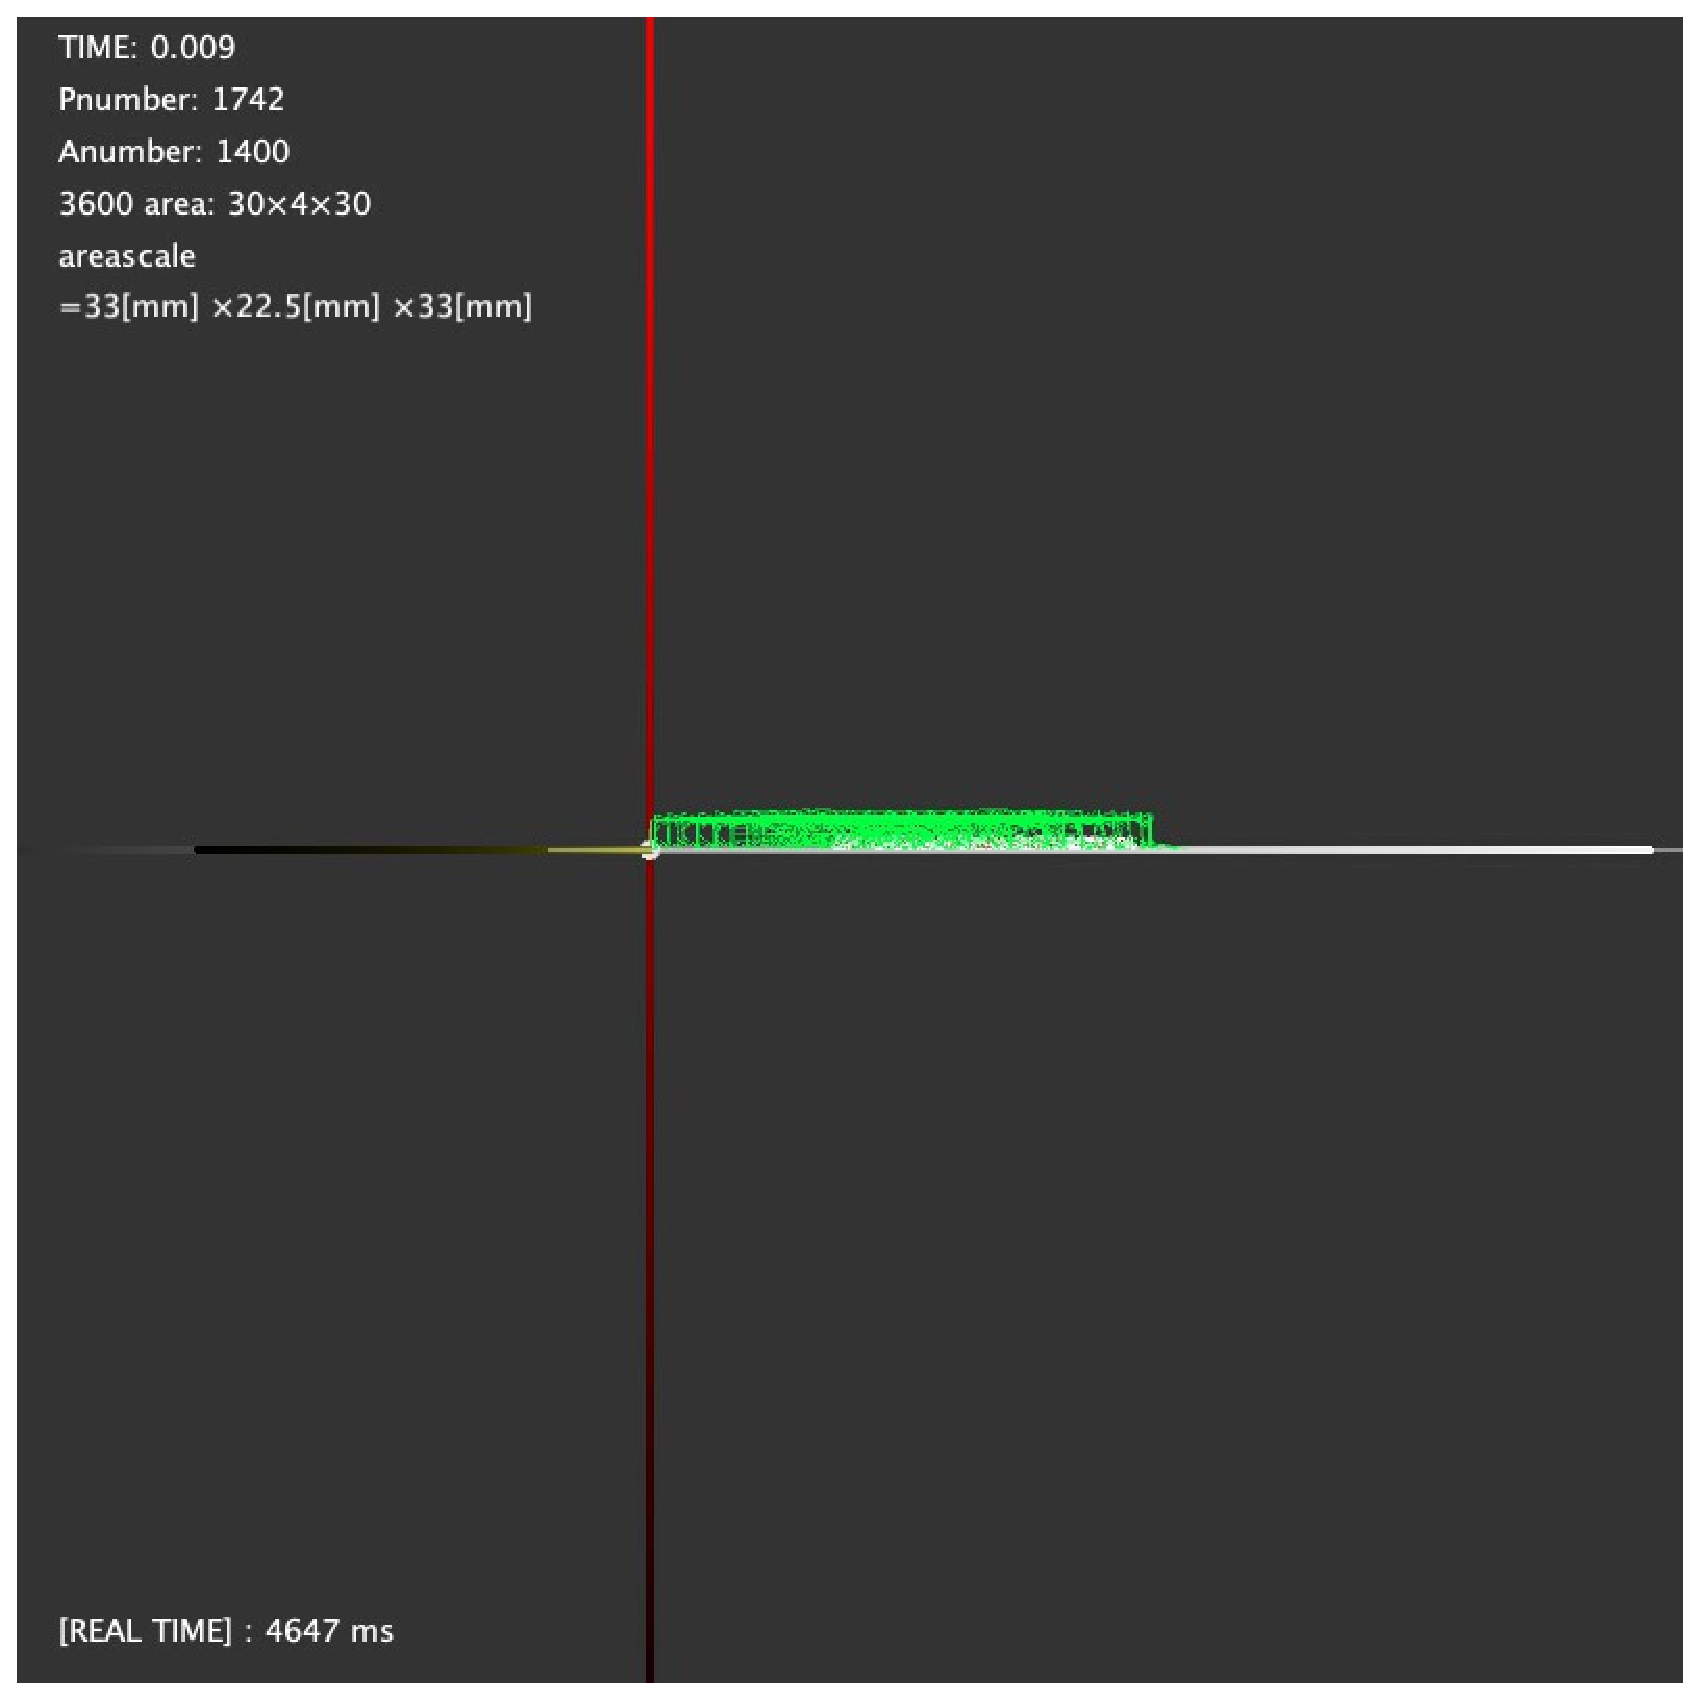
\includegraphics[width=5cm]{side.eps} 
  \end{tabular}
 }%
  \caption{Initial state. (a)~Top view. Green lines and white dots show actin molecules and membrane particles, respectively. (b)~Side view.}
 \label{fig:ini}
\end{figure}
The number of actin molecules and membrane particles were 1,000 and 1,618, respectively, in the computer simulation.
The positions of membrane particles were updated every step of the numerical computation and the positions of actin molecules were updated every 10 steps.

Fig. \ref{fig:ini} shows the initial state of the virtual cell of  the computer simulation.
The actin molecule are in a U-shaped area excluding the rear of the cell (Fig. \ref{fig:ini}).
The membrane molecules were placed on the surface of the cylinder.

\chapter{Results and Discussion}
\section{Simulation Results}
\subsection{Role of Actin Retrograde Flow}
%SF、距離非依存
\begin{figure}[tbp]
 \subfloat[]{%
  \begin{tabular}{c}
   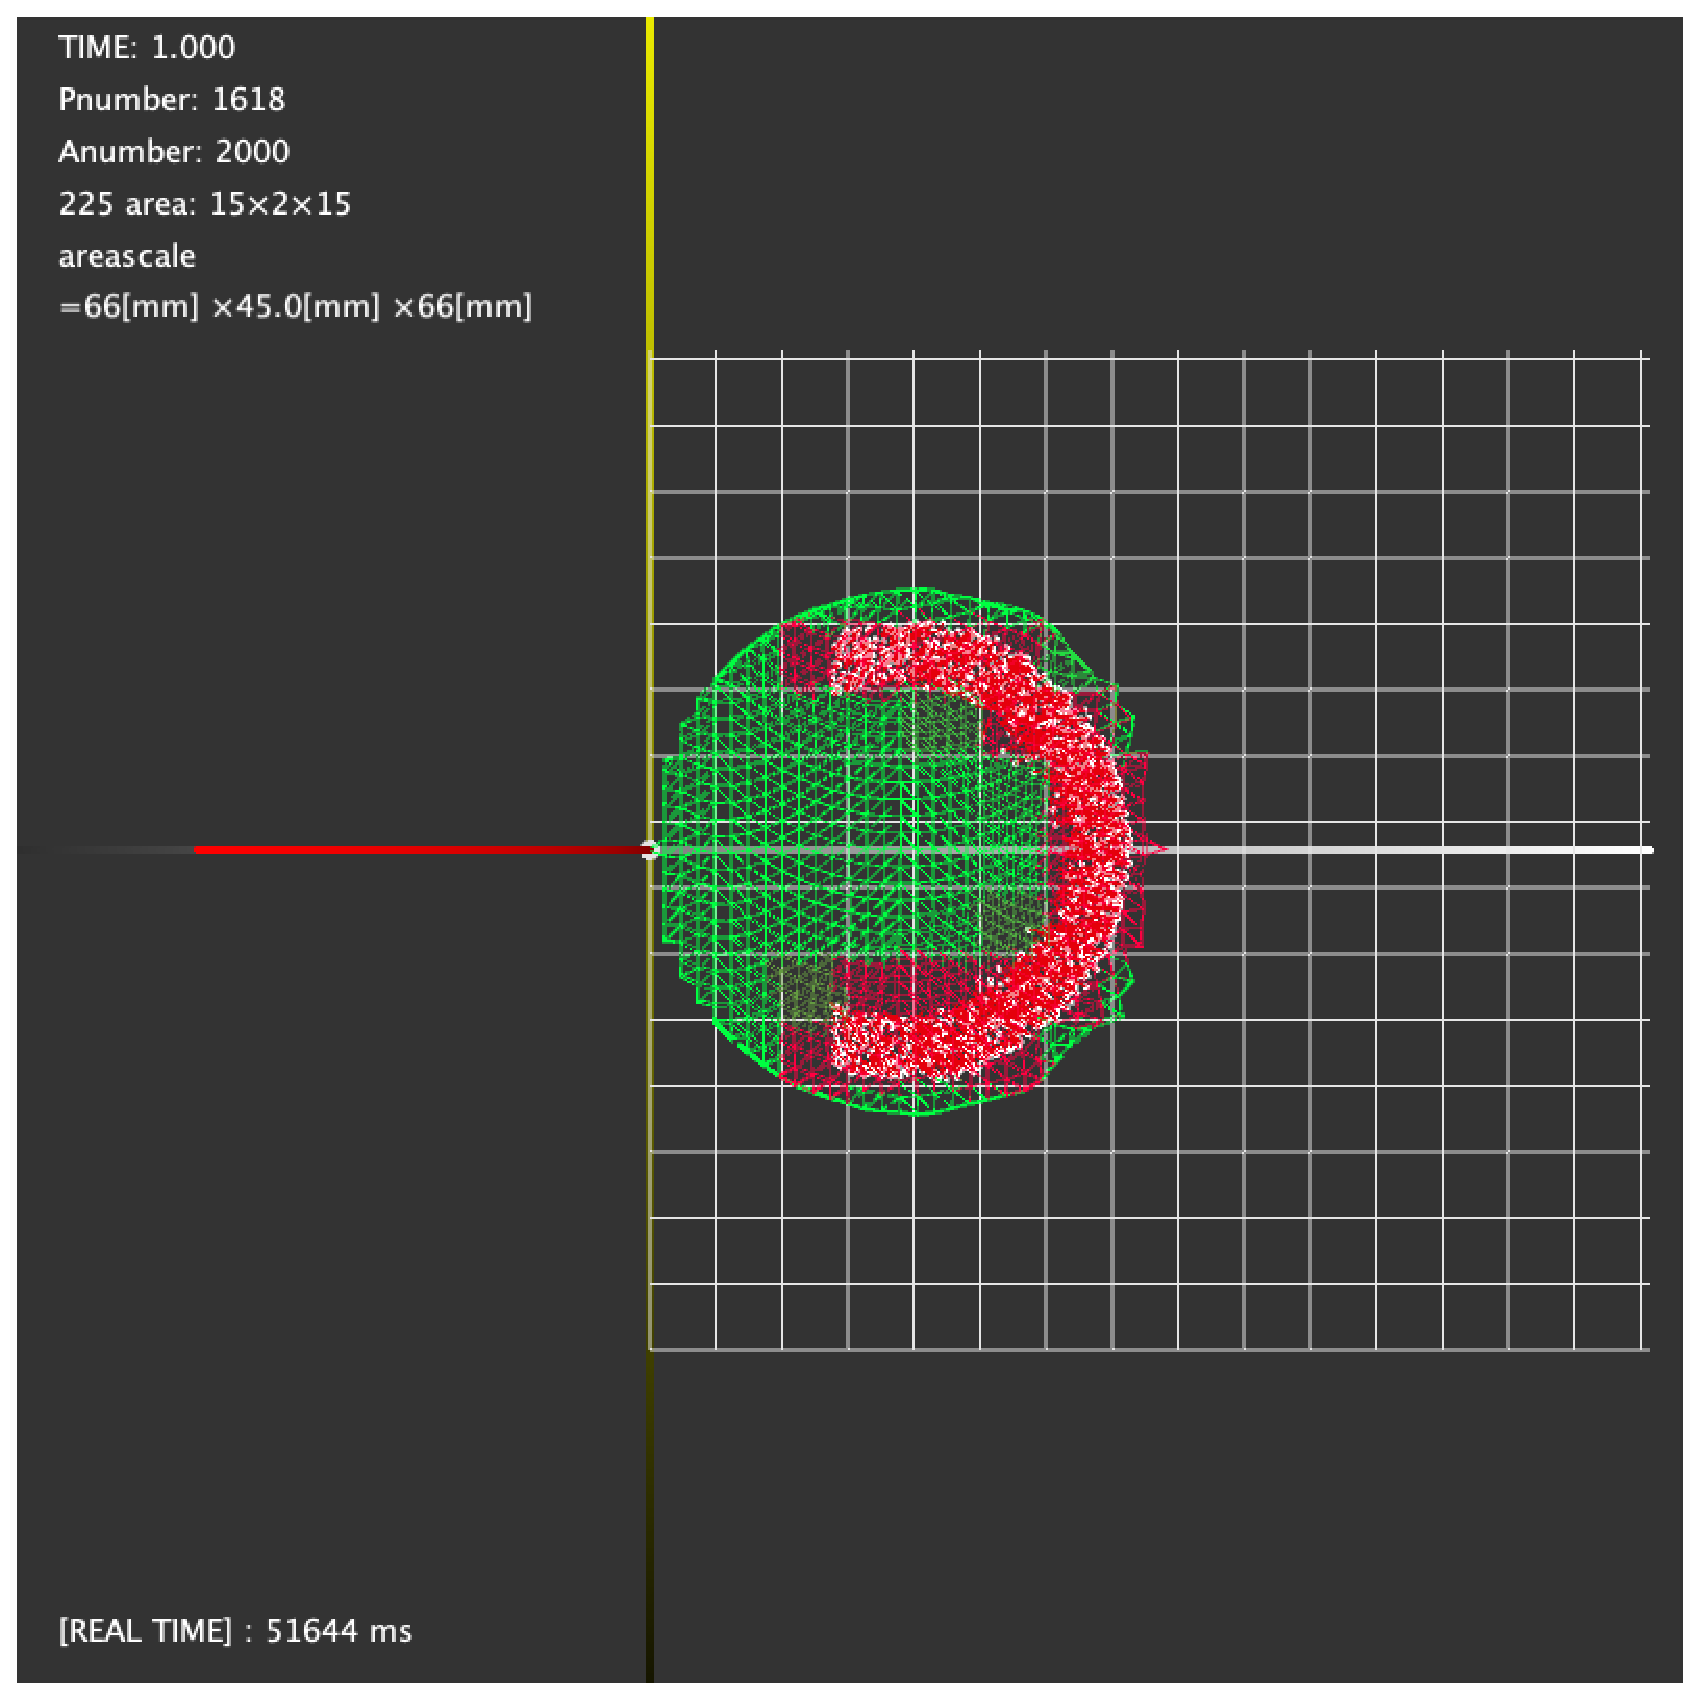
\includegraphics[width=5cm]{10_arf.eps} 
  \end{tabular}
 }%
 \subfloat[]{%
  \begin{tabular}{c}
   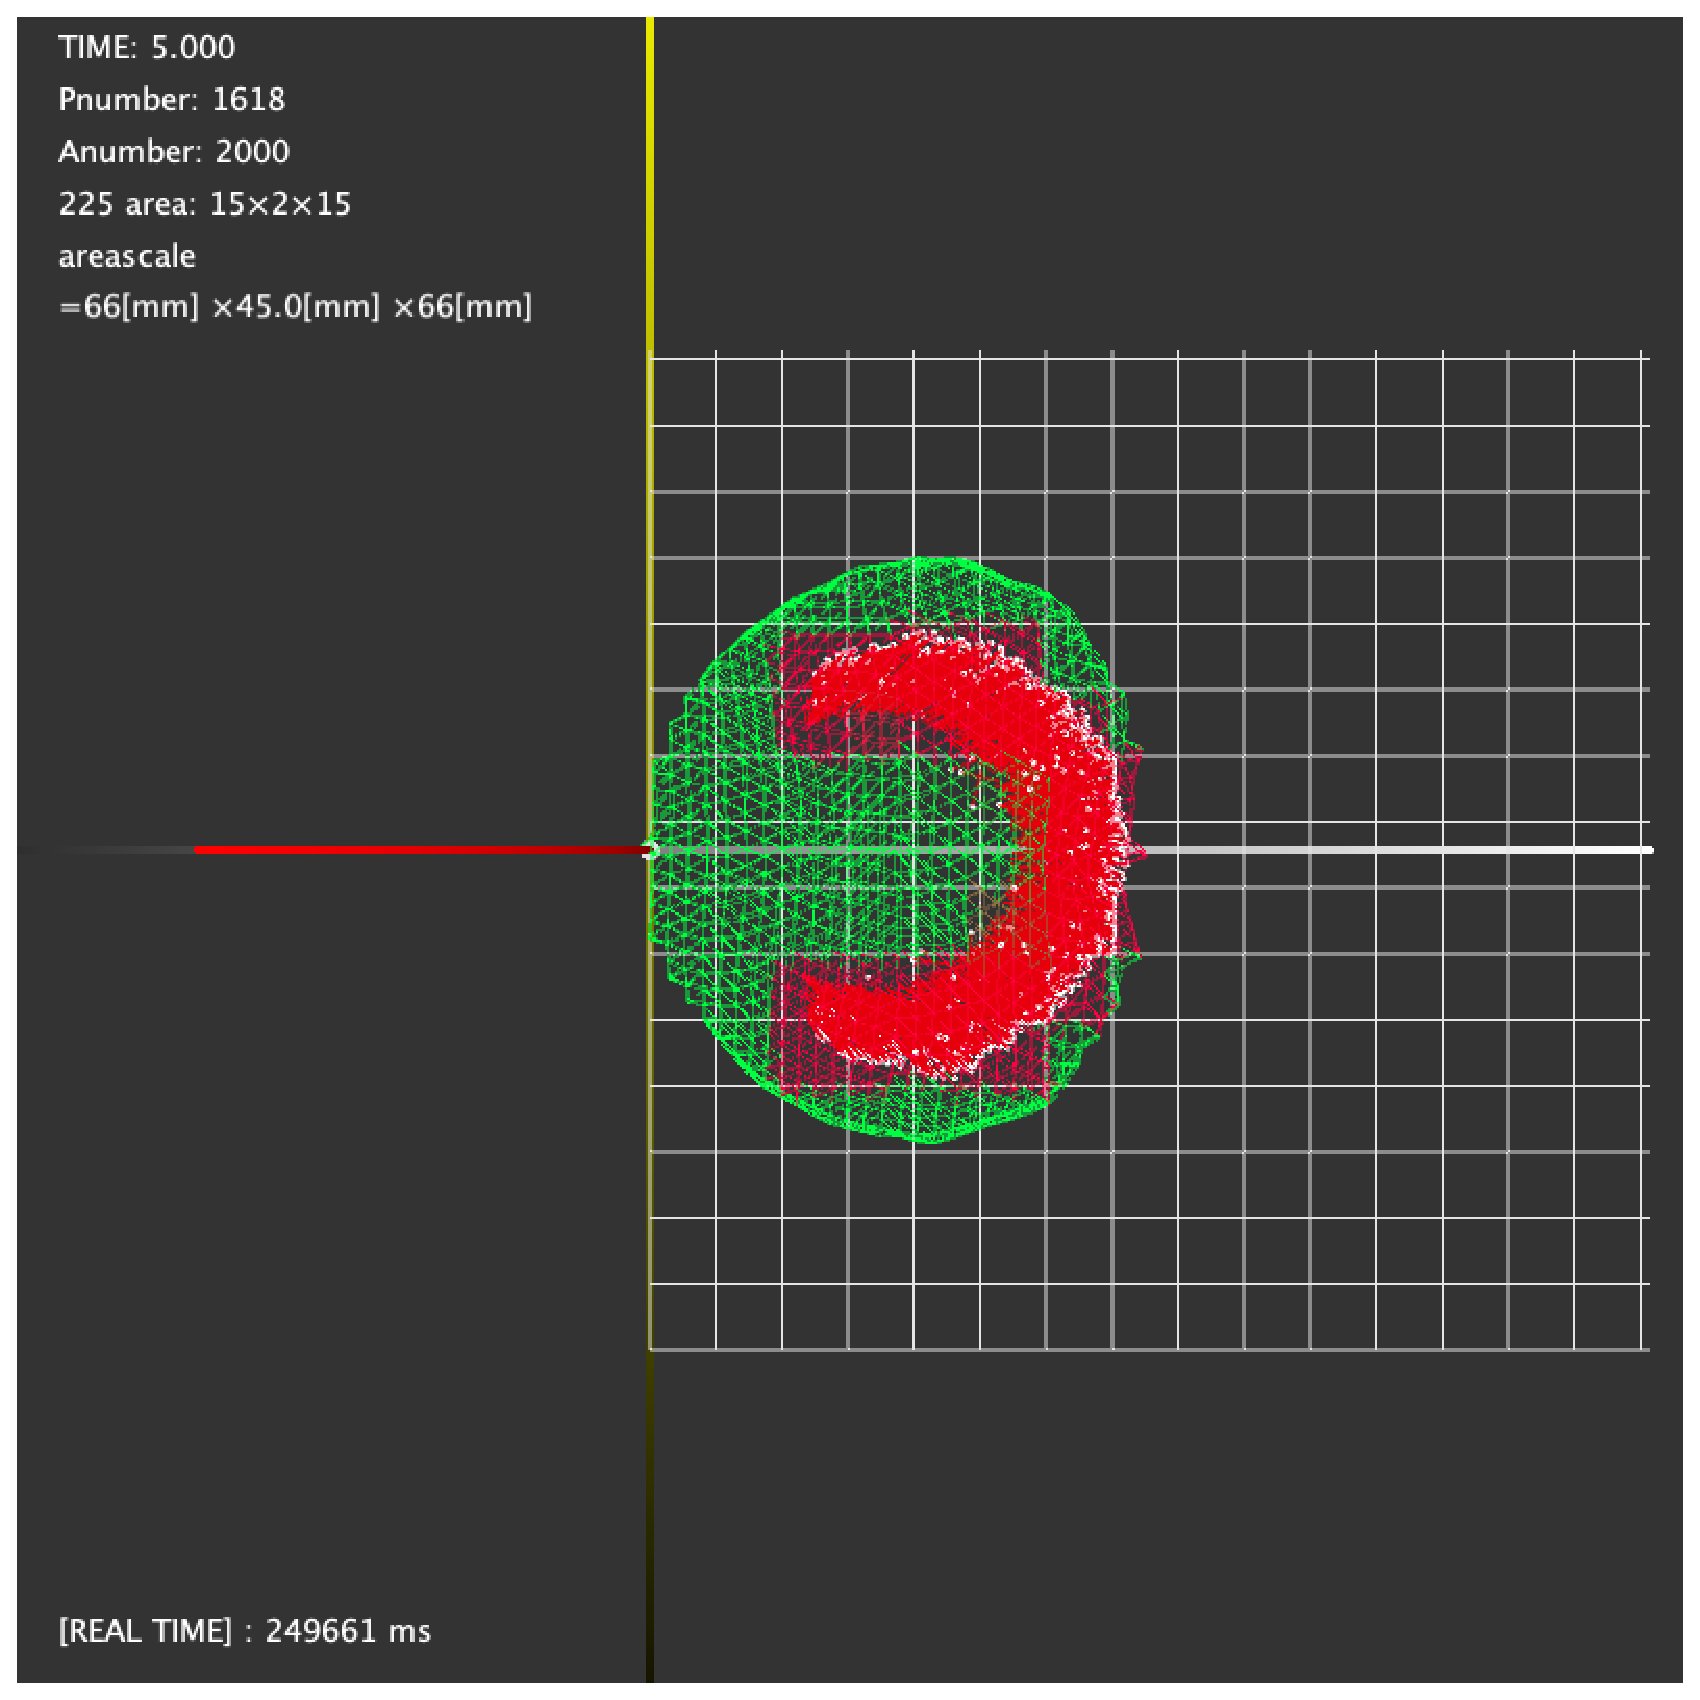
\includegraphics[width=5cm]{50_arf.eps} 
  \end{tabular}
 }%
 \subfloat[]{%
  \begin{tabular}{c}
   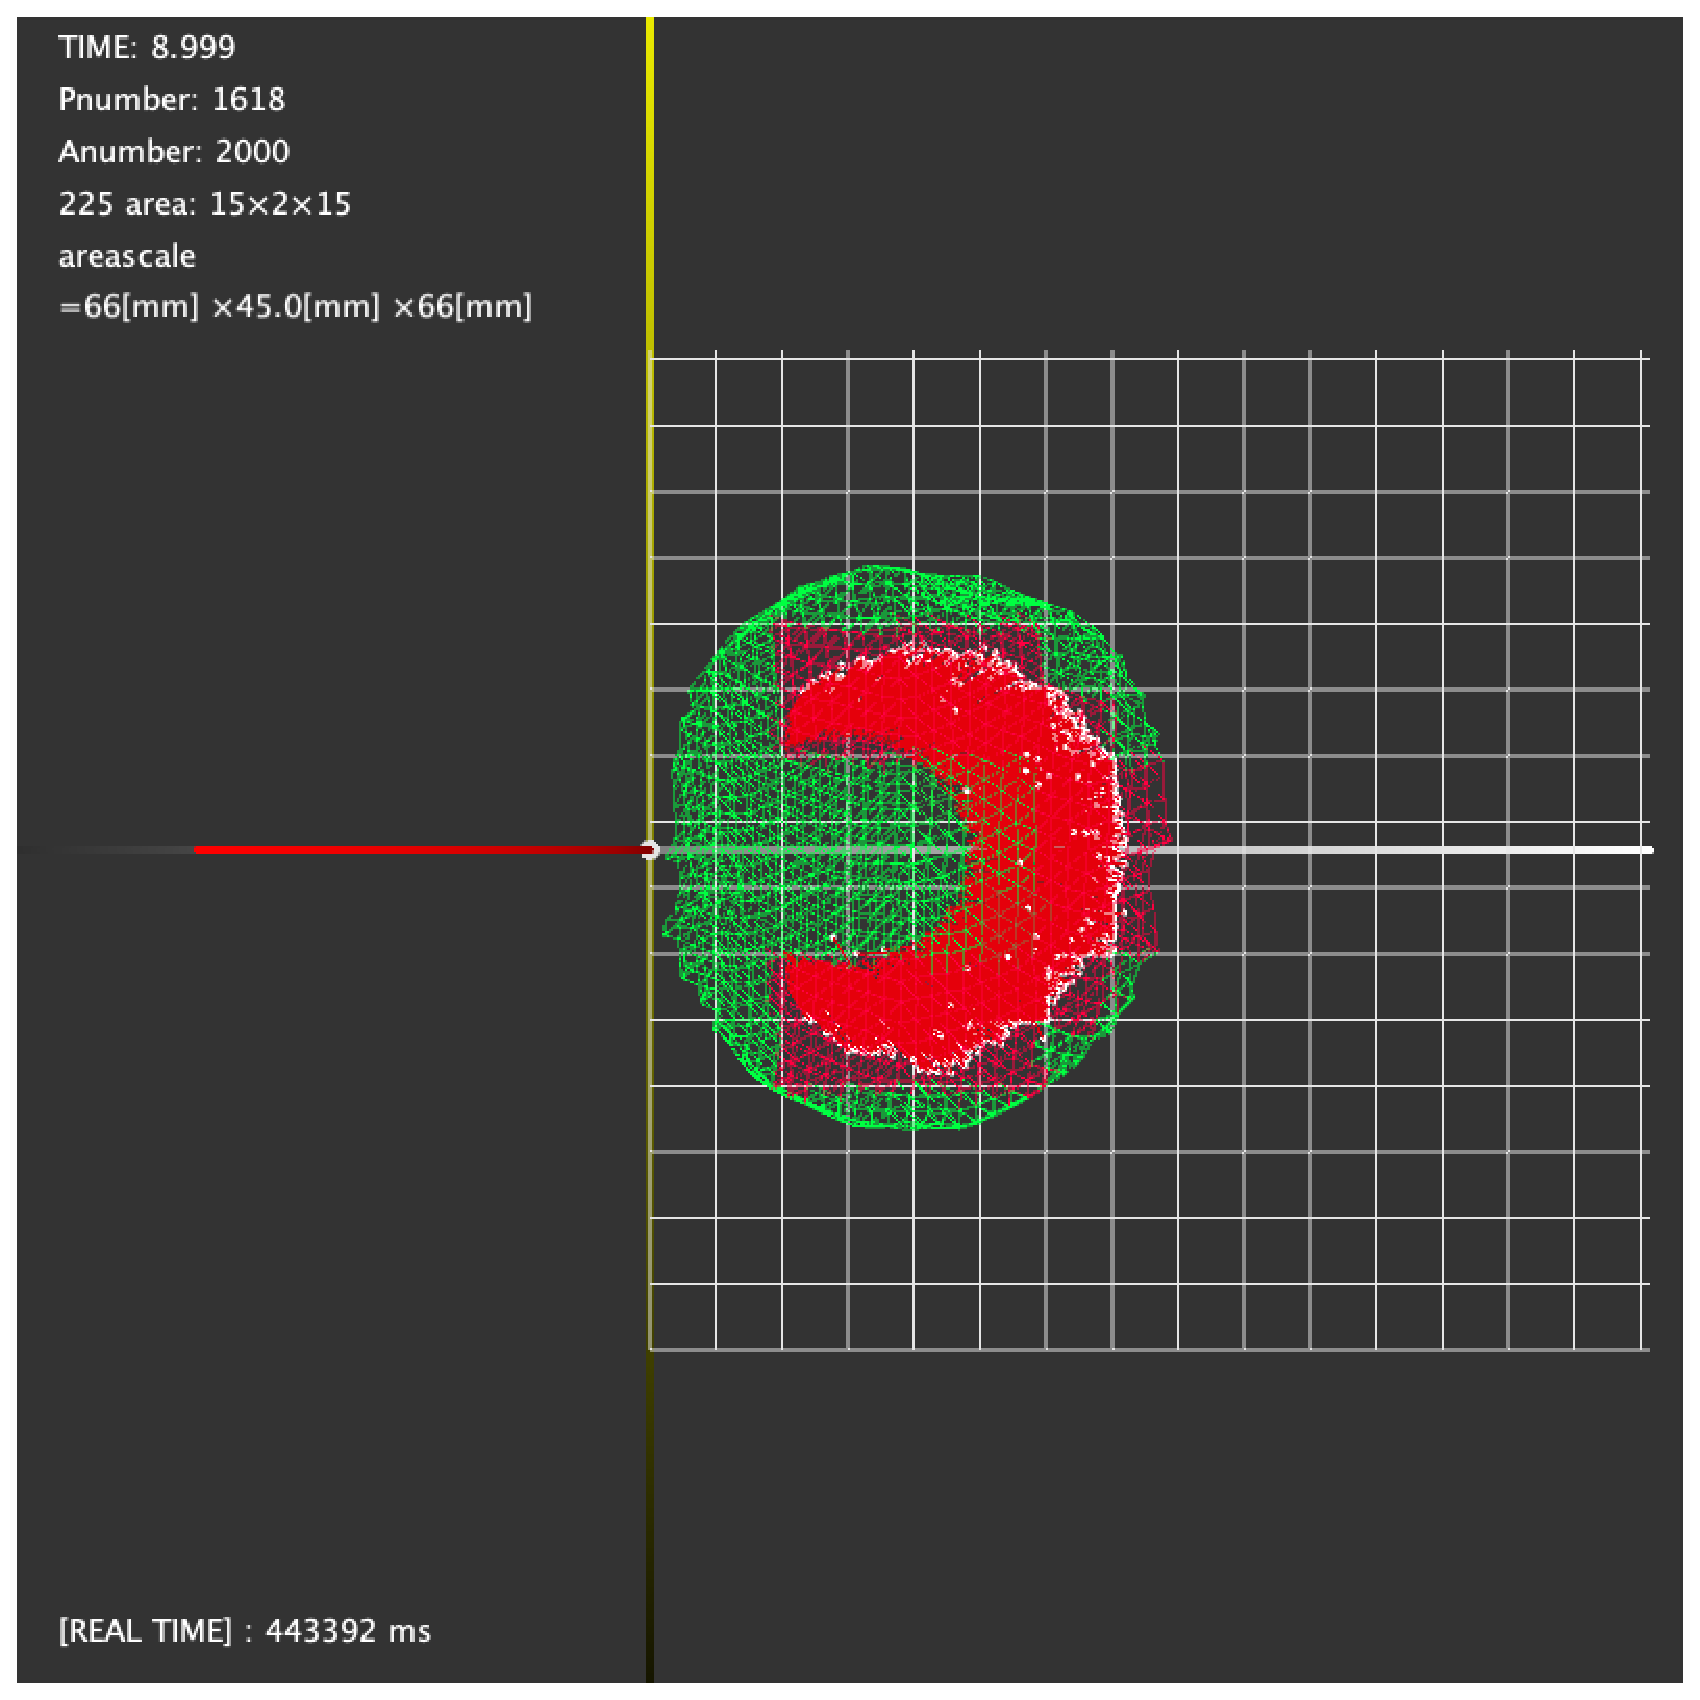
\includegraphics[width=5cm]{90_arf.eps} 
  \end{tabular}
 }%
 \caption{Simulation results when the amplitude of the retraction by the ARF is independent of the distance. (a), (b), and (c) show the results at $t = 1.0, 6.0, 11.0$~[s]. Green lines show the cell membrane, and white and red dots show the barbed-end of the F-actin, respectively.}
 \label{fig:res0}
\end{figure}

%SF、距離依存
\begin{figure}[tbp]
 \subfloat[]{%
  \begin{tabular}{c}
   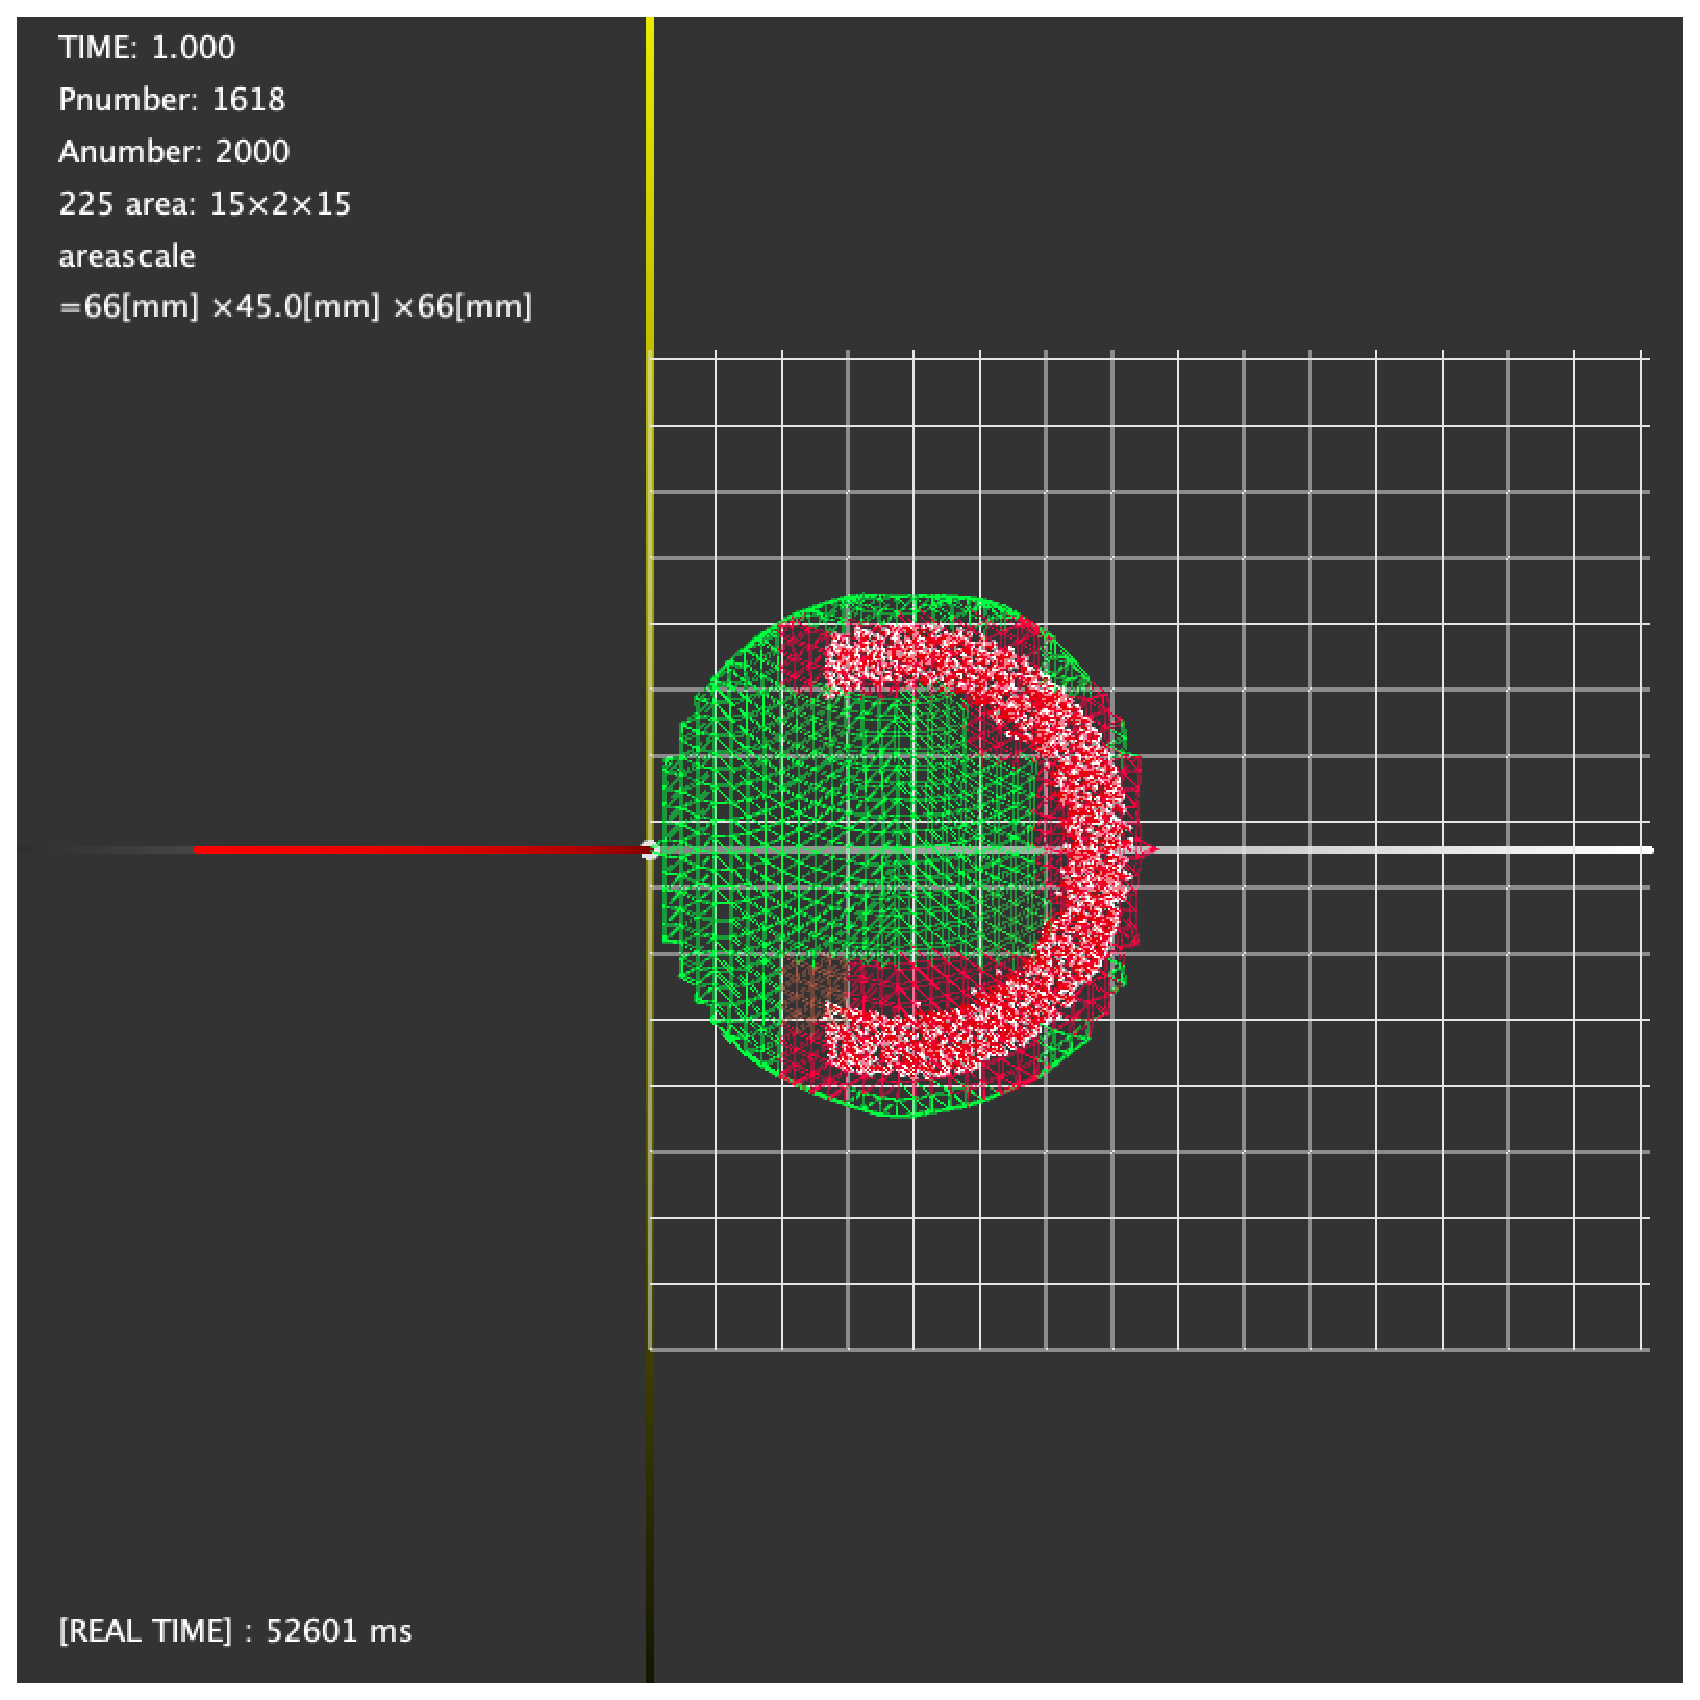
\includegraphics[width=5cm]{10_darf.eps} 
  \end{tabular}
 }%
 \subfloat[]{%
  \begin{tabular}{c}
   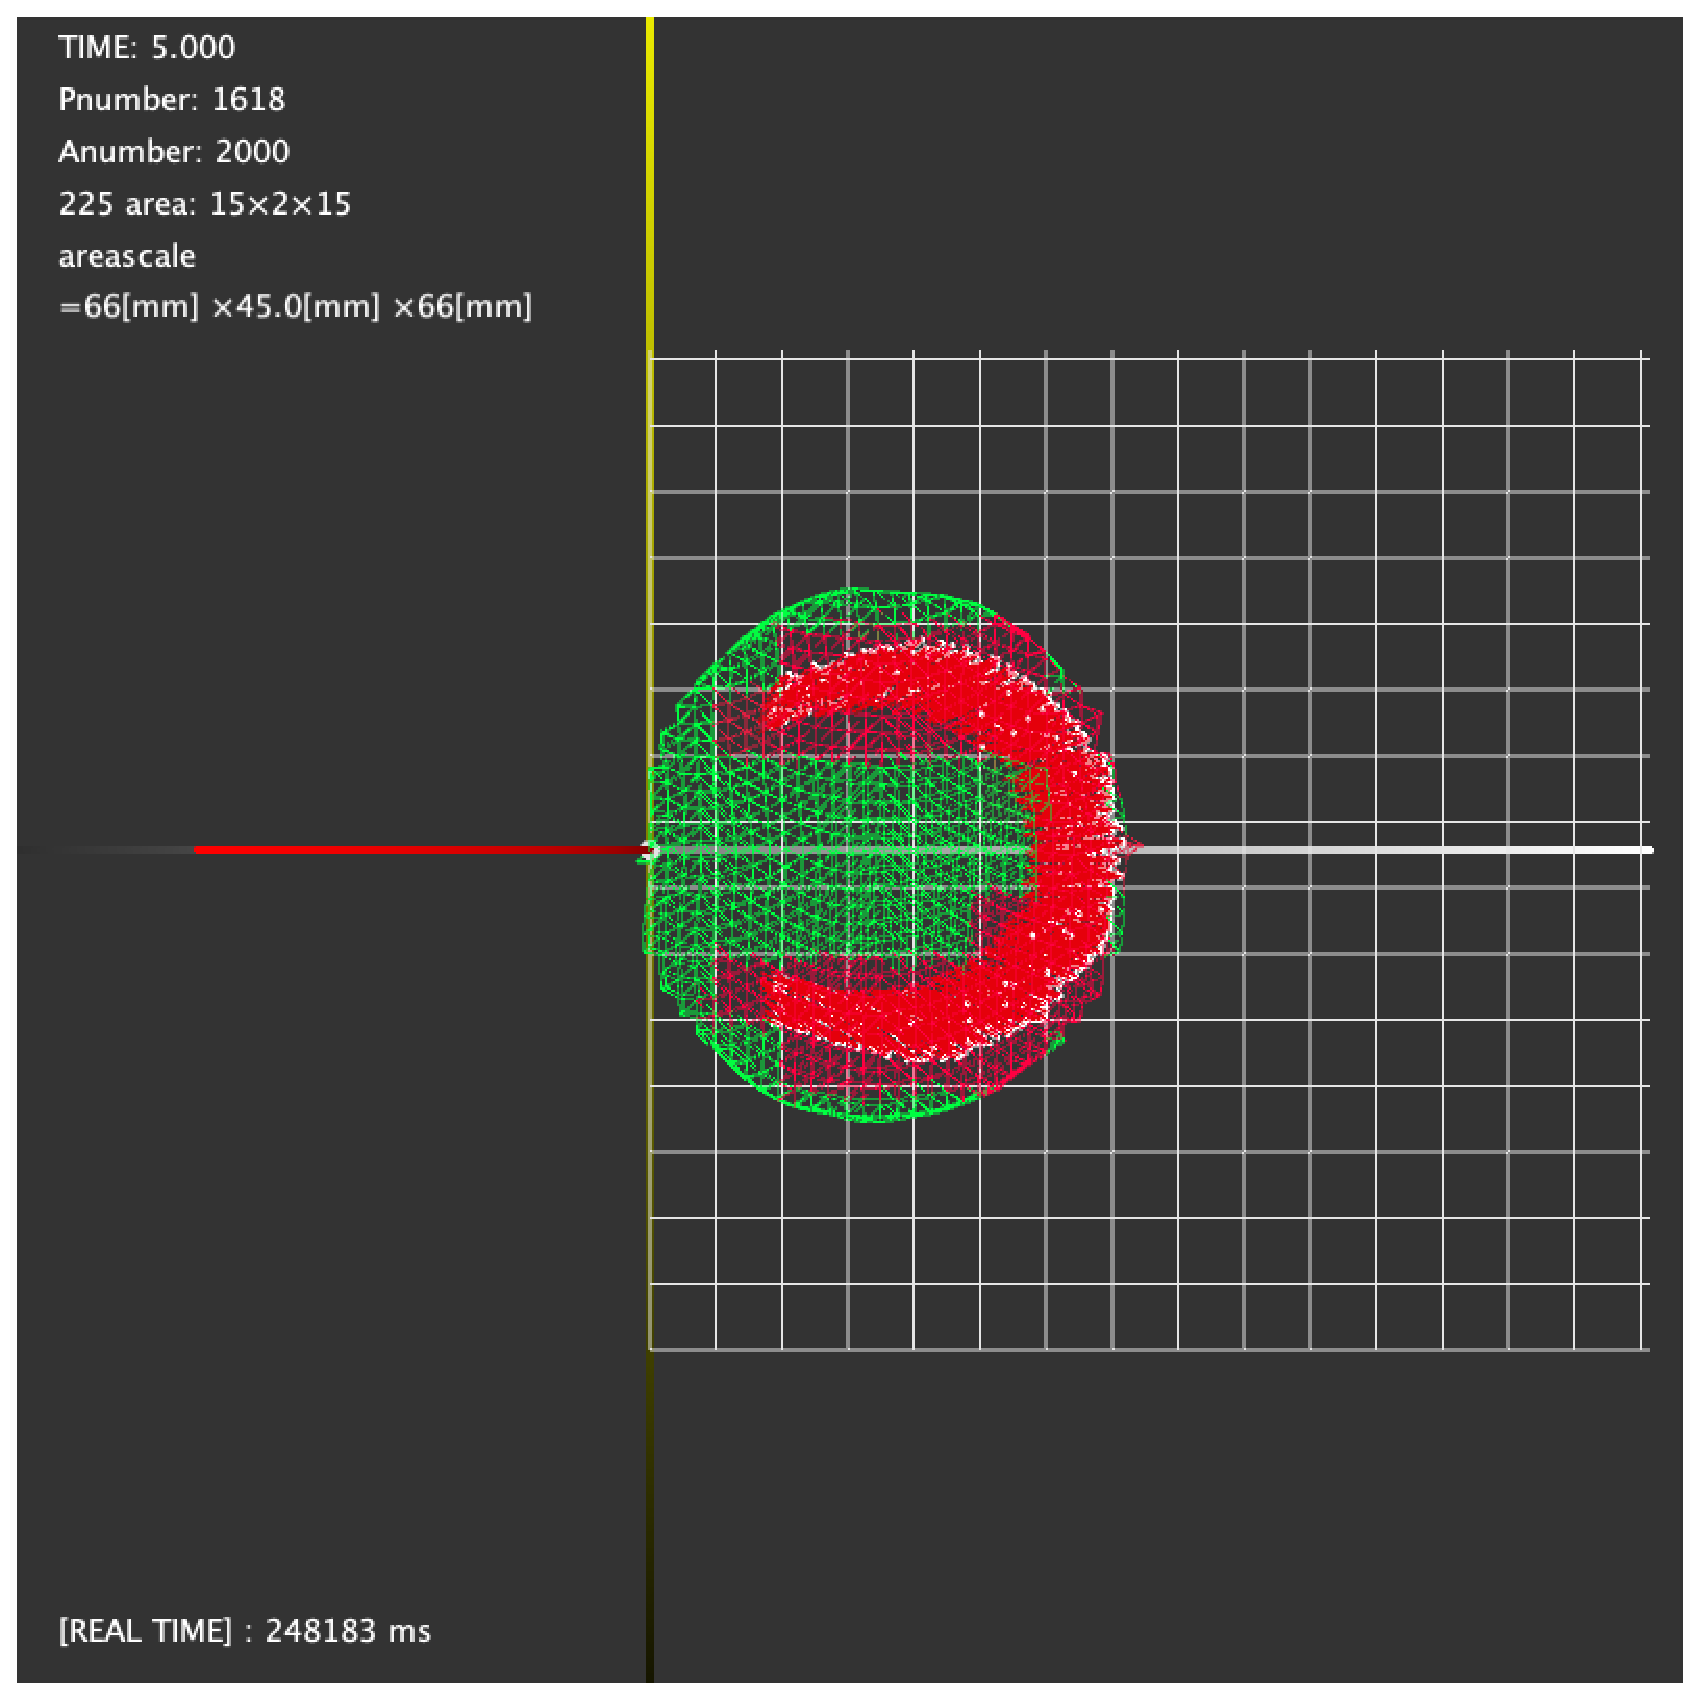
\includegraphics[width=5cm]{50_darf.eps} 
  \end{tabular}
 }%
 \subfloat[]{%
  \begin{tabular}{c}
   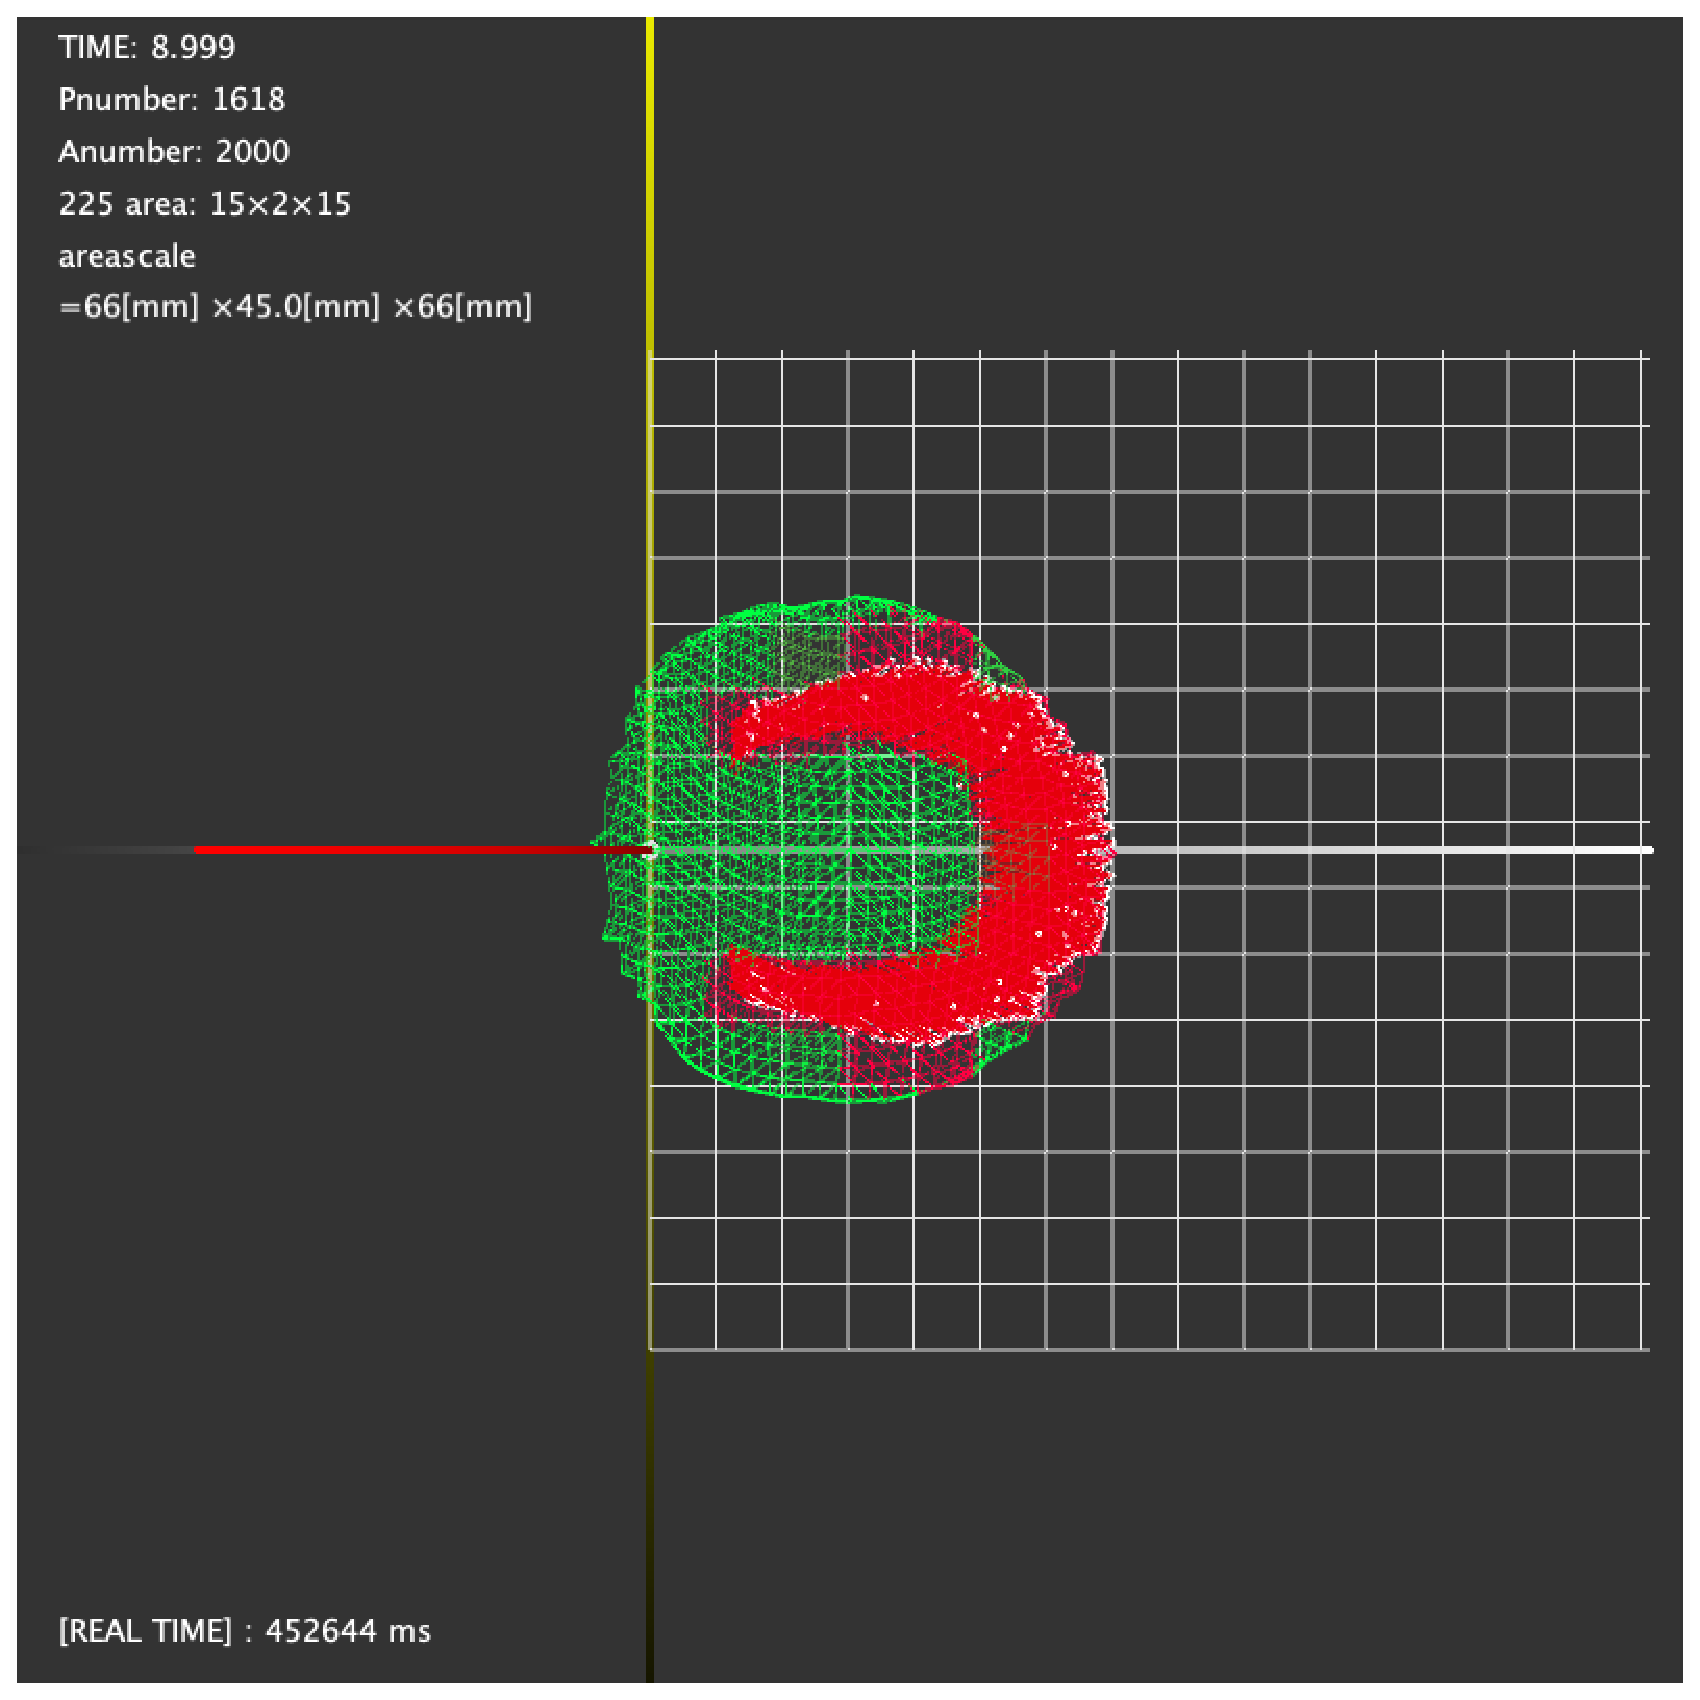
\includegraphics[width=5cm]{90_darf.eps} 
  \end{tabular}
 }%
 \caption{Simulation results under the same codition as those in Fig. \ref{fig:res0} except $w=2$ in eq. (\ref{eq:arf}).~The subfigures show the results at different timings as in Fig. \ref{fig:res0}.}
 \label{fig:res1}
\end{figure}

%RP、距離非依存
\begin{figure}[tbp]
 \subfloat[]{%
  \begin{tabular}{c}
   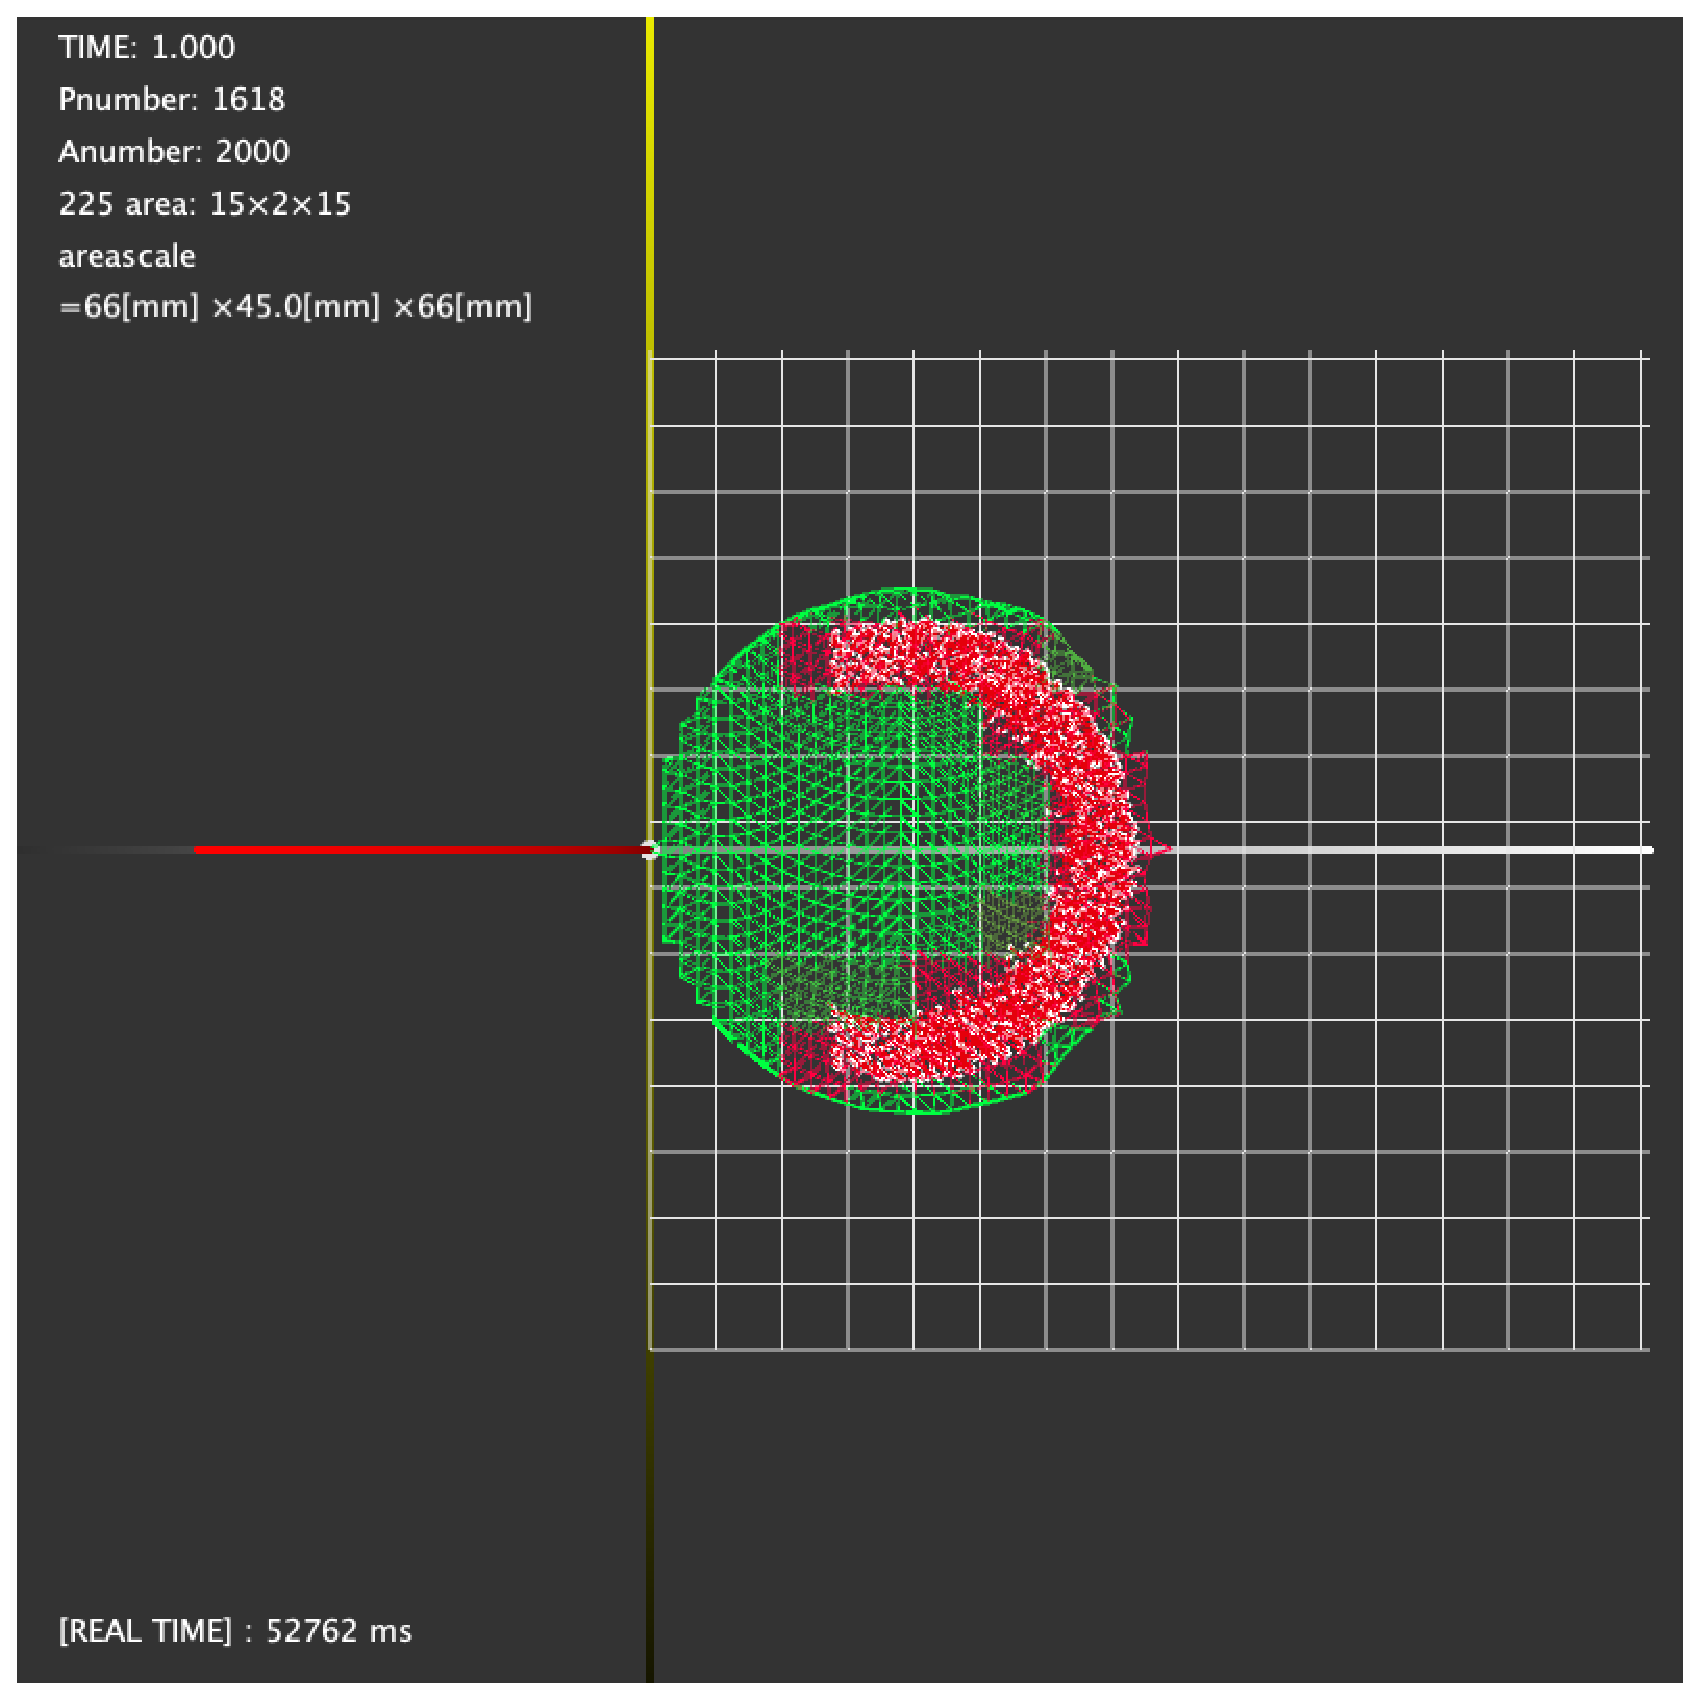
\includegraphics[width=5cm]{10_1arf.eps} 
  \end{tabular}
 }%
 \subfloat[]{%
  \begin{tabular}{c}
   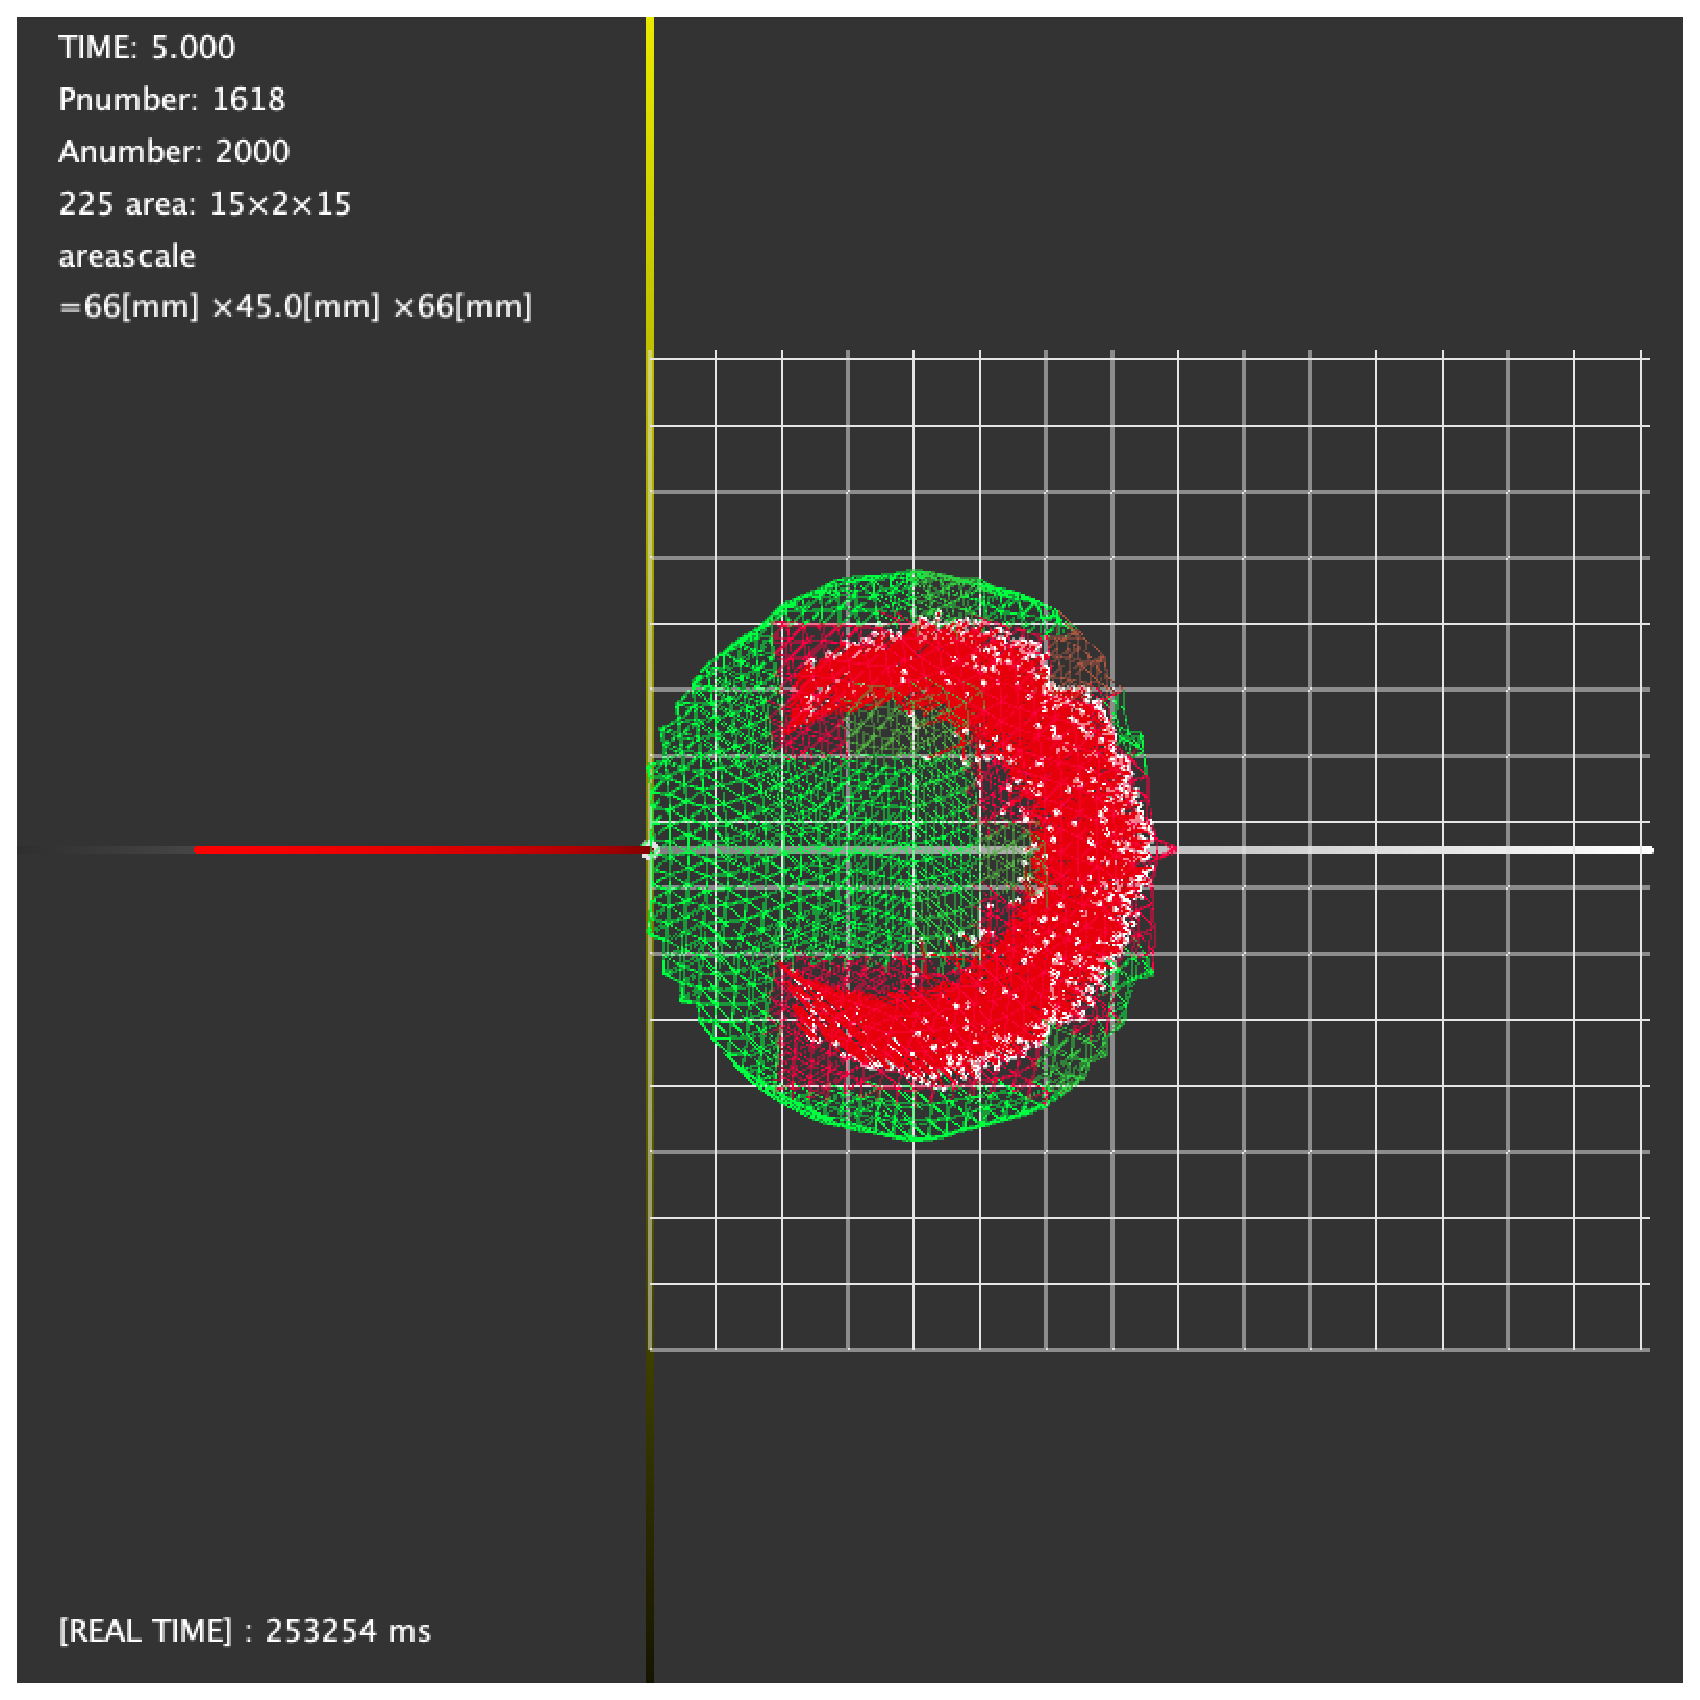
\includegraphics[width=5cm]{50_1arf.eps}
  \end{tabular}
 }%
 \subfloat[]{%
  \begin{tabular}{c}
   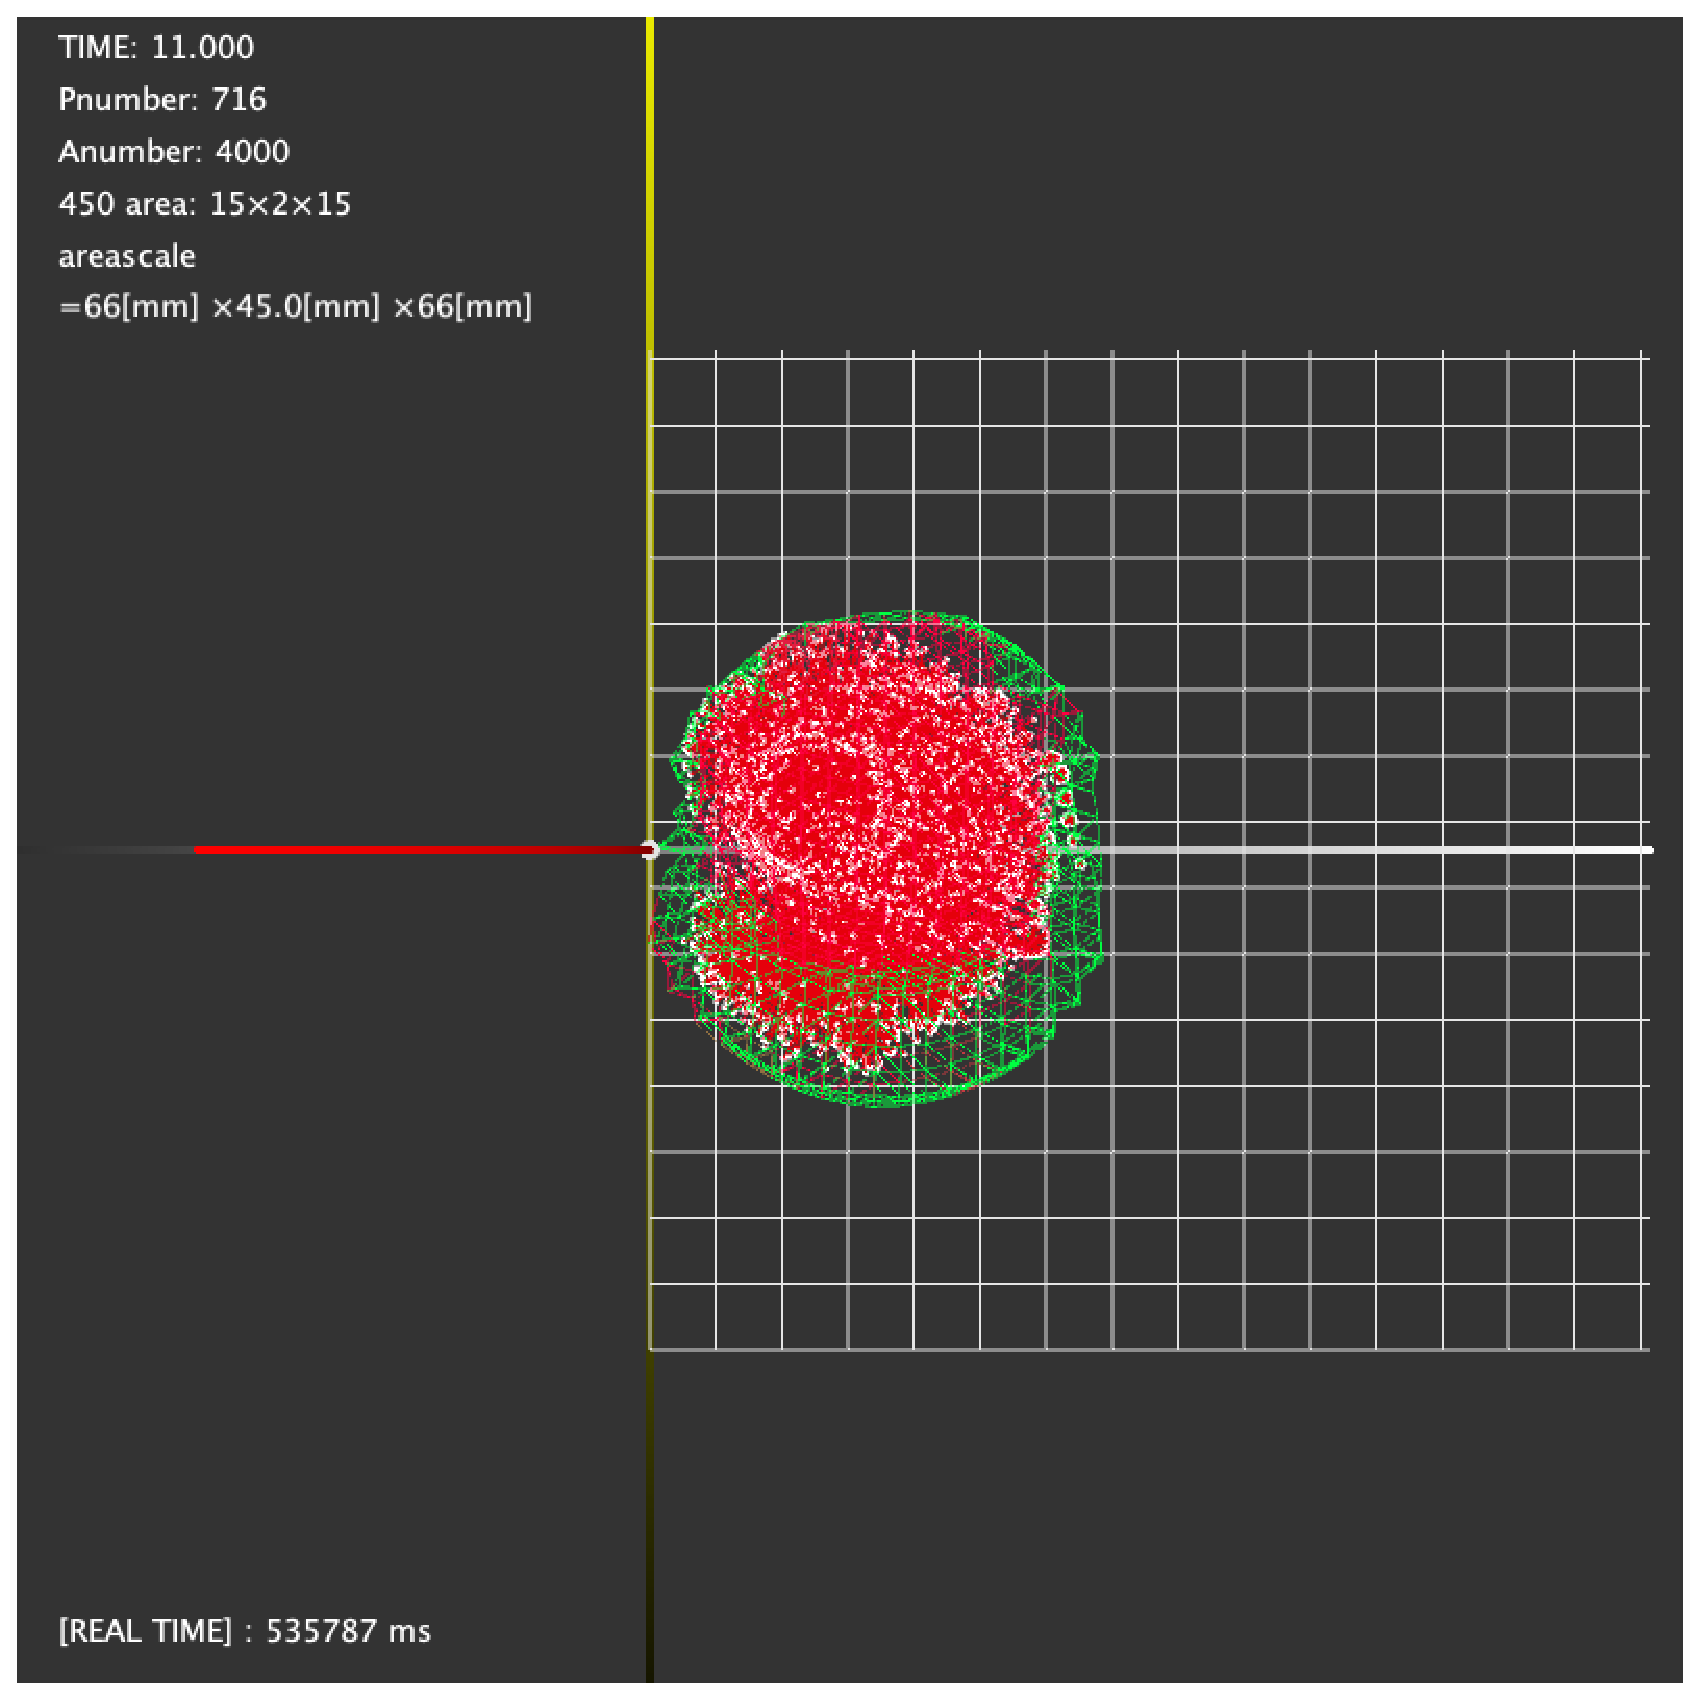
\includegraphics[width=5cm]{90_1arf.eps} 
  \end{tabular}
 }%
 \caption{Simulation results when the reference point of the ARF was  assumed at  the position of the leftmost membrane molecule of the cell. The subfigures show the results at different timings as in Fig. \ref{fig:res0}.}
 \label{fig:res2}
\end{figure}

%NON ARF

\begin{figure}[tbp]
 \subfloat[]{%
  \begin{tabular}{c}
   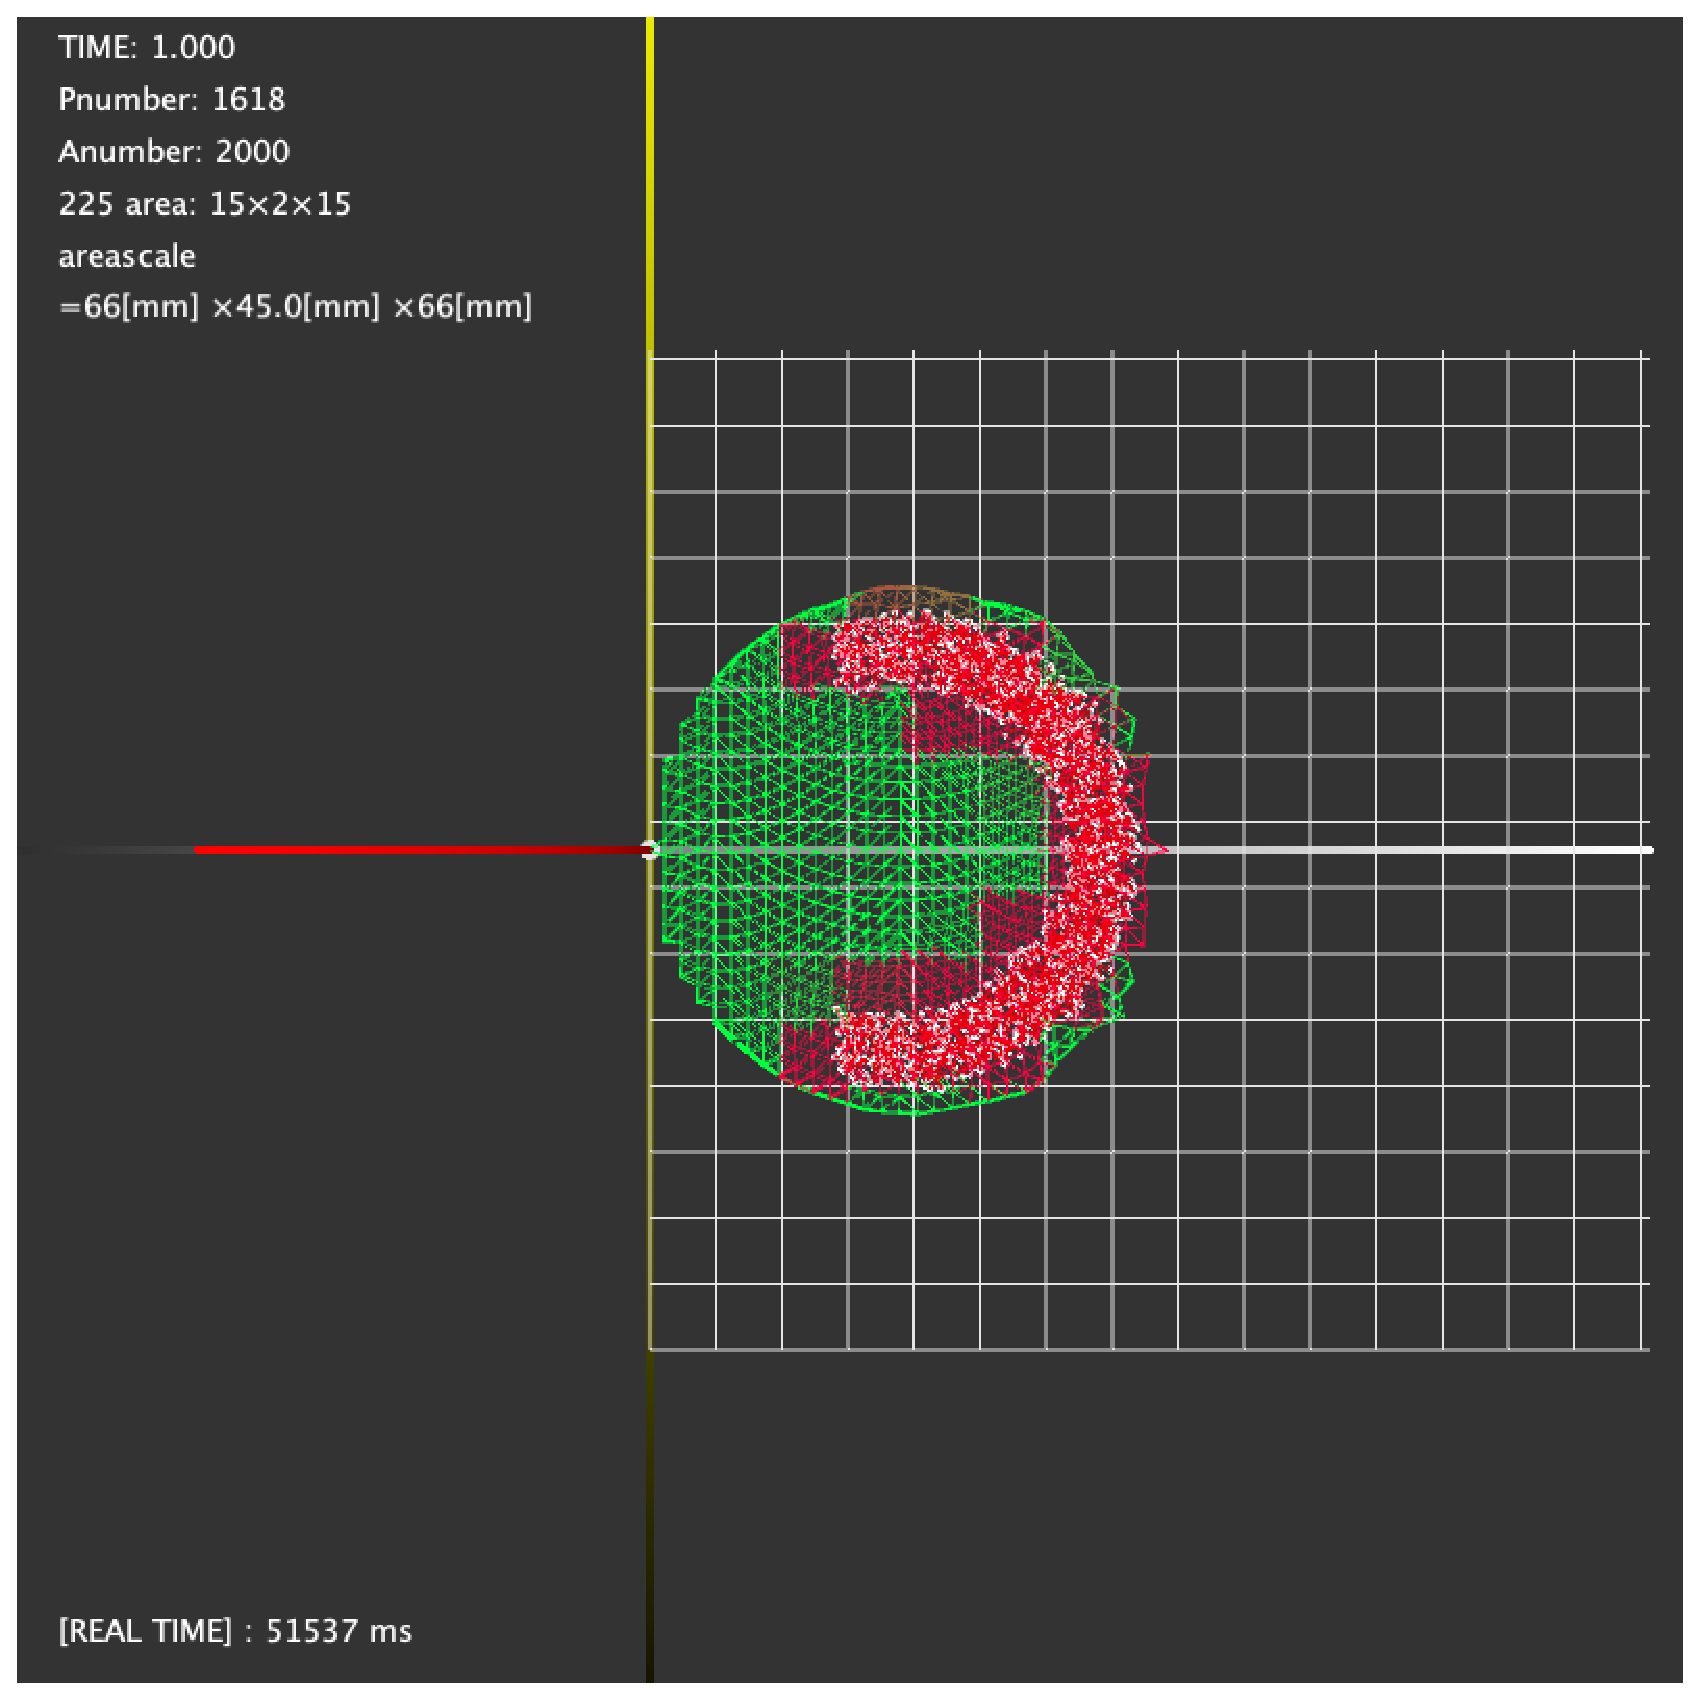
\includegraphics[width=5cm]{10_narf.eps} 
  \end{tabular}
 }%
 \subfloat[]{%
  \begin{tabular}{c}
   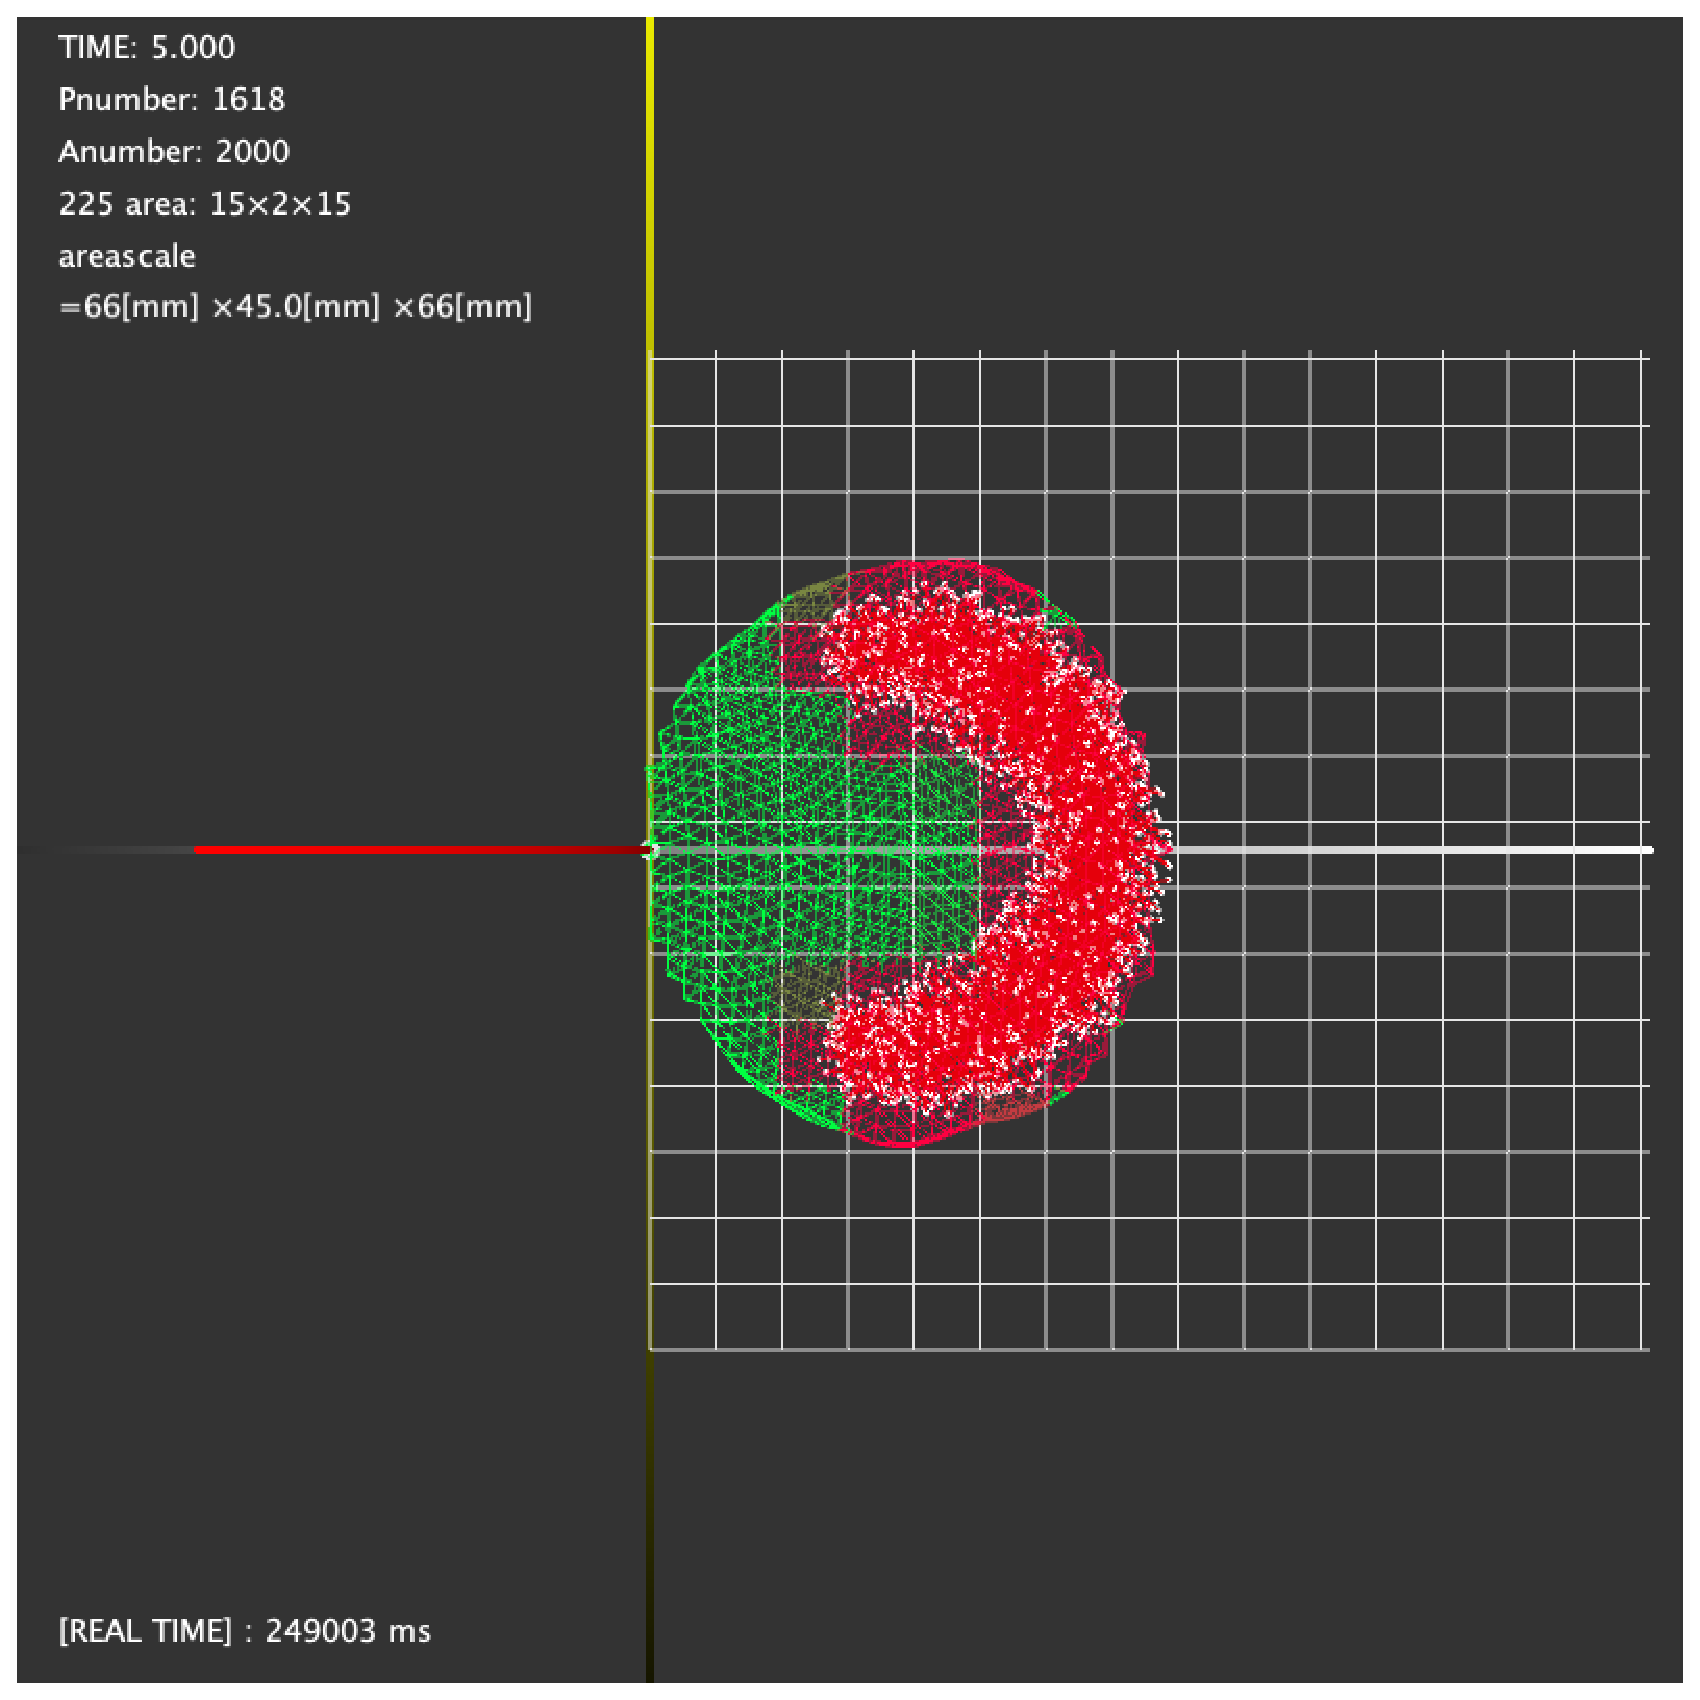
\includegraphics[width=5cm]{50_narf.eps}
  \end{tabular}
 }%
 \subfloat[]{%
  \begin{tabular}{c}
   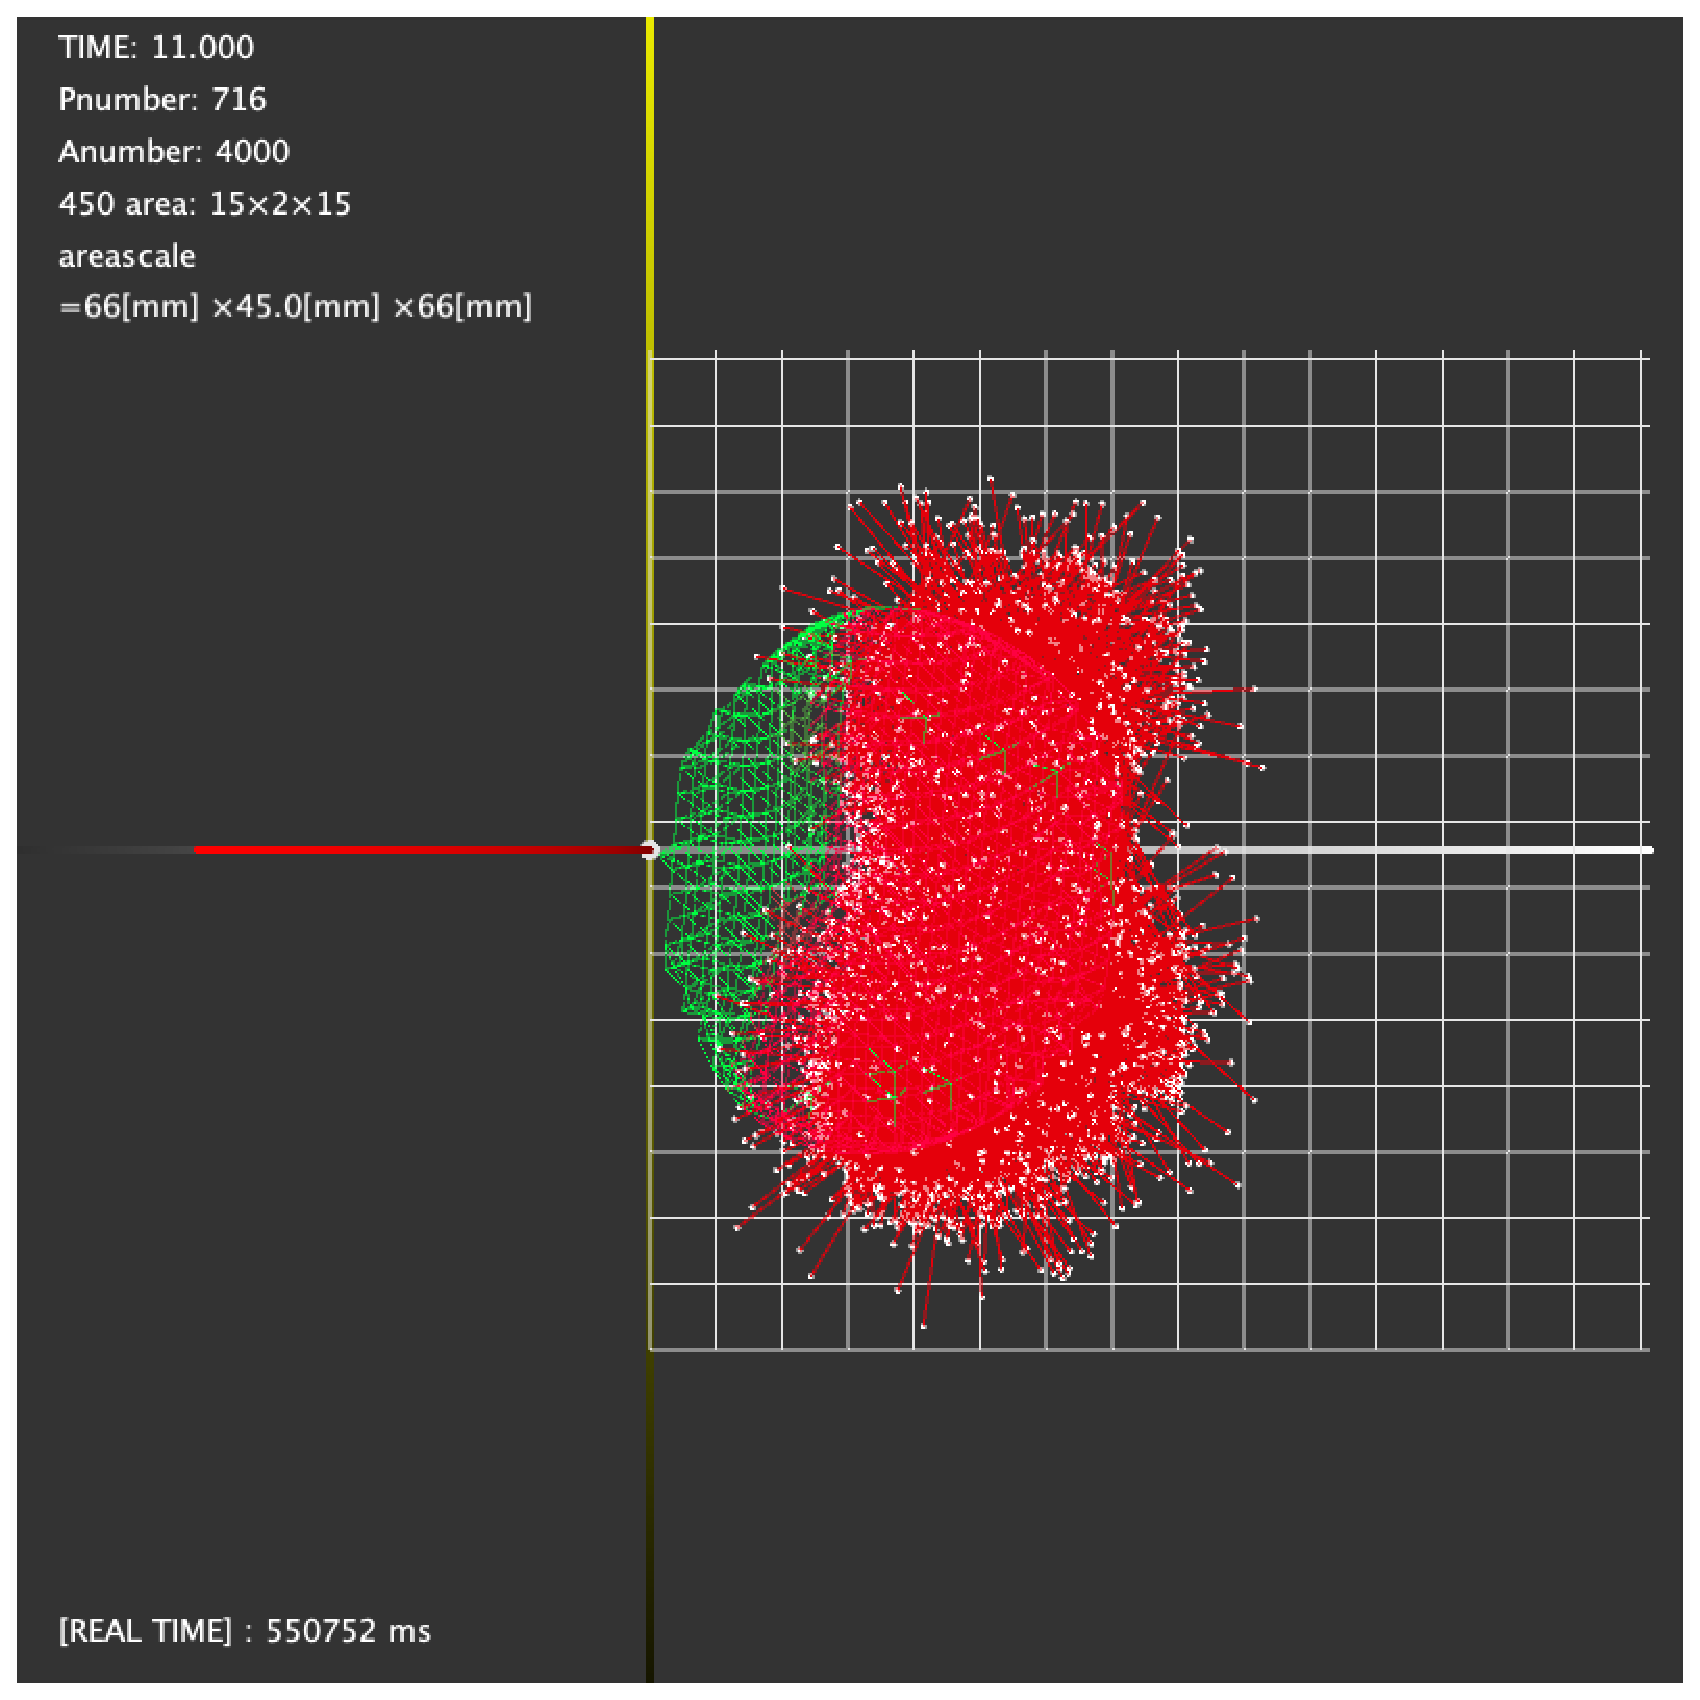
\includegraphics[width=5cm]{90_narf.eps} 
  \end{tabular}
 }%
 \caption{Simulation Results without the ARF. The subfigures show the results at different timings as in Fig. \ref{fig:res0}.}
 \label{fig:res3}
\end{figure}

\begin{figure}[tbp]
 \subfloat[]{%
  \begin{tabular}{c}
   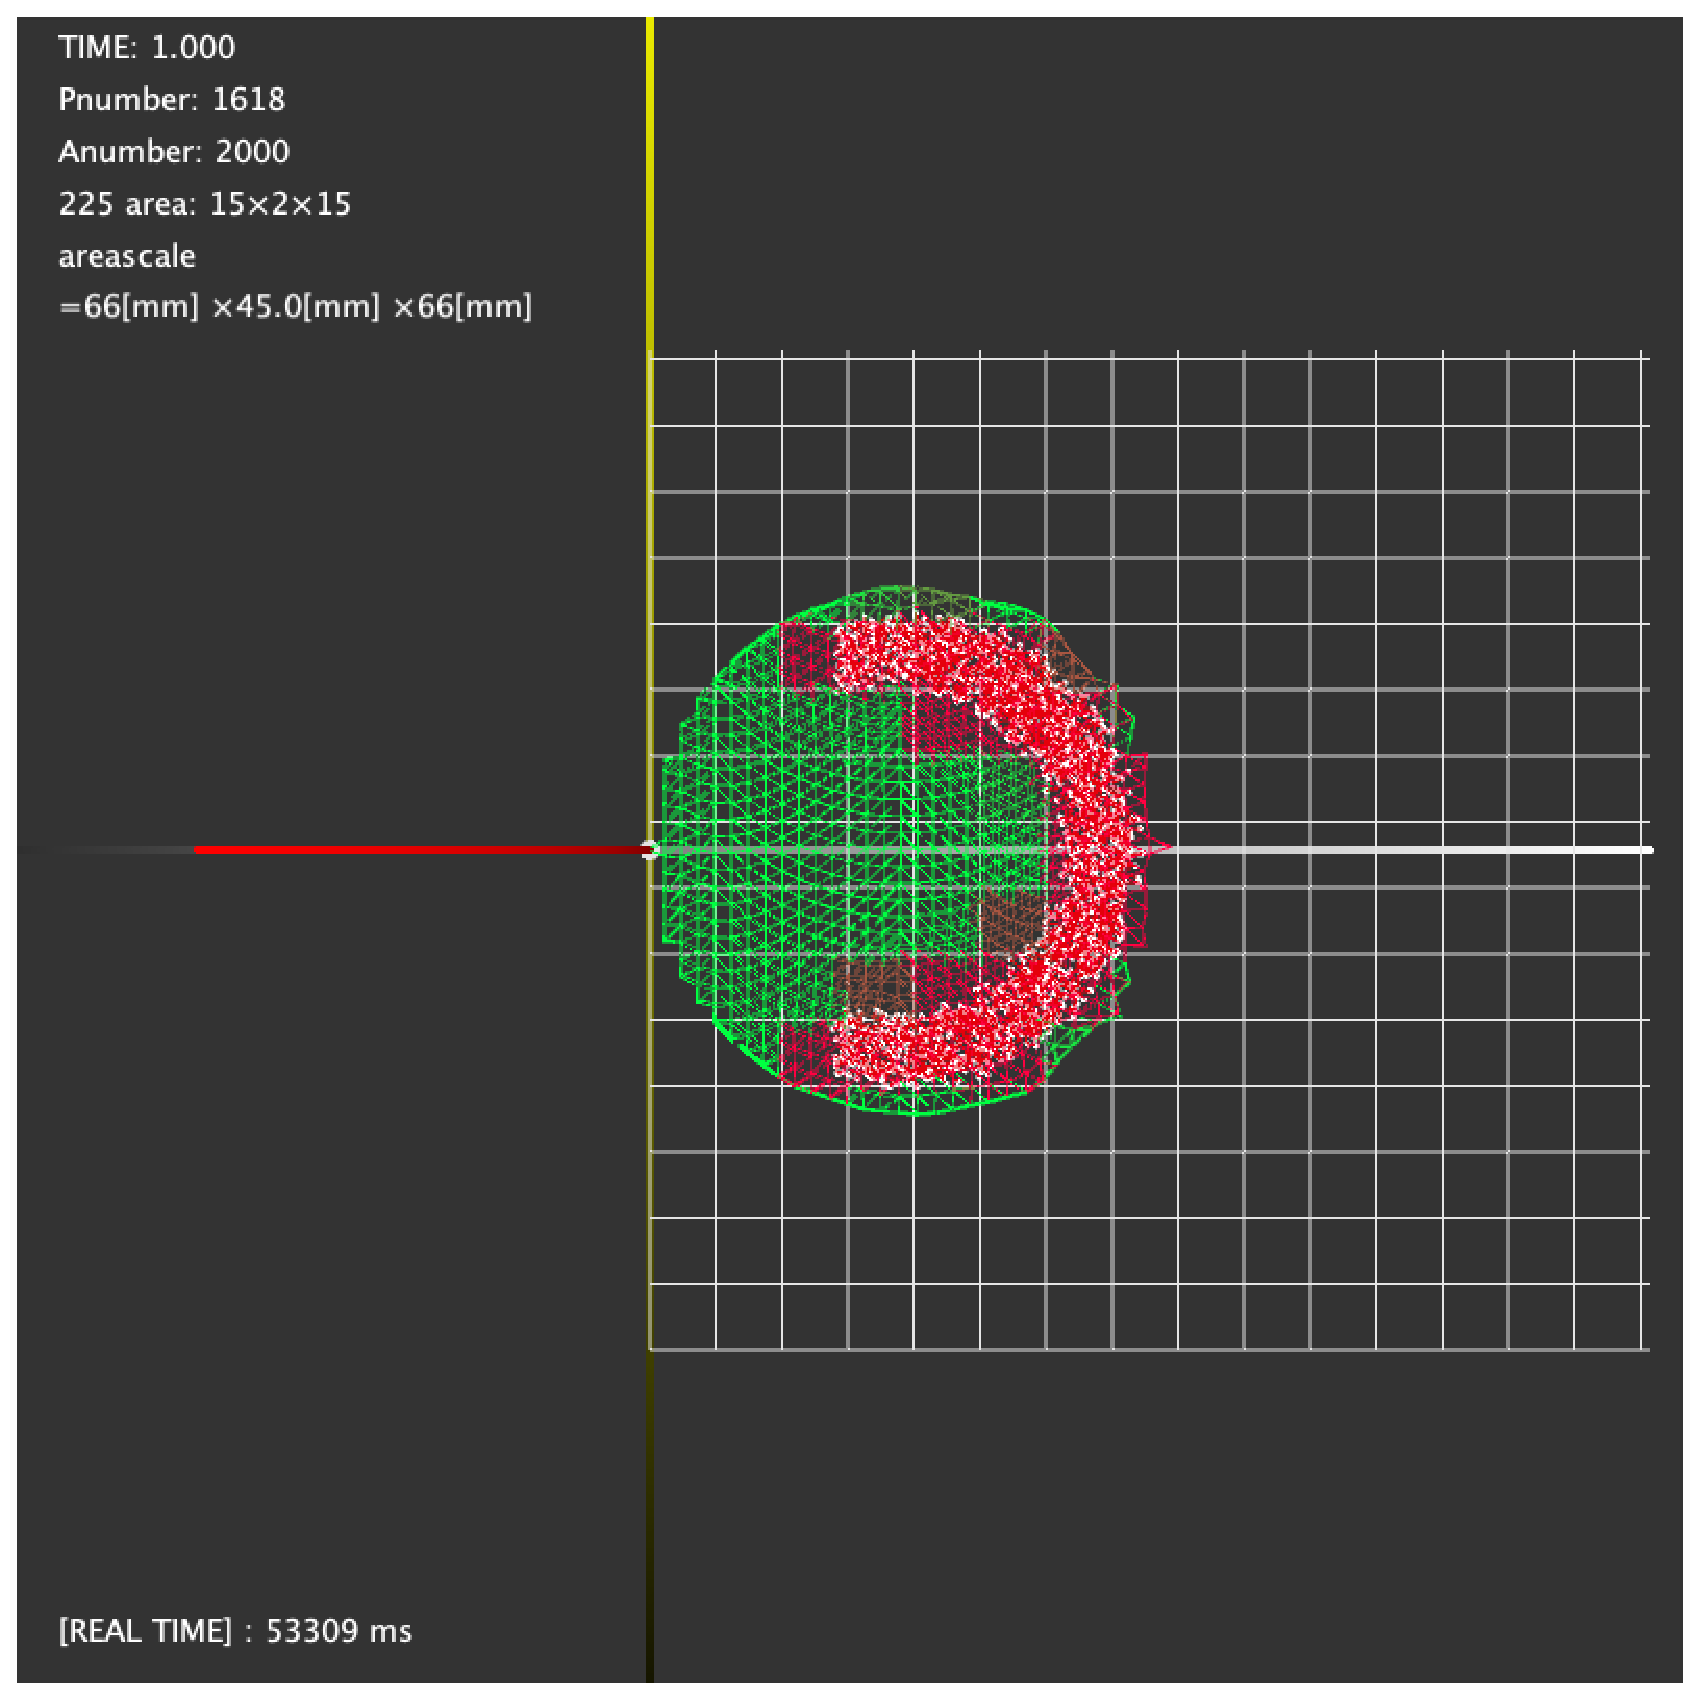
\includegraphics[width=5cm]{10_nro.eps} 
  \end{tabular}
 }%
 \subfloat[]{%
  \begin{tabular}{c}
   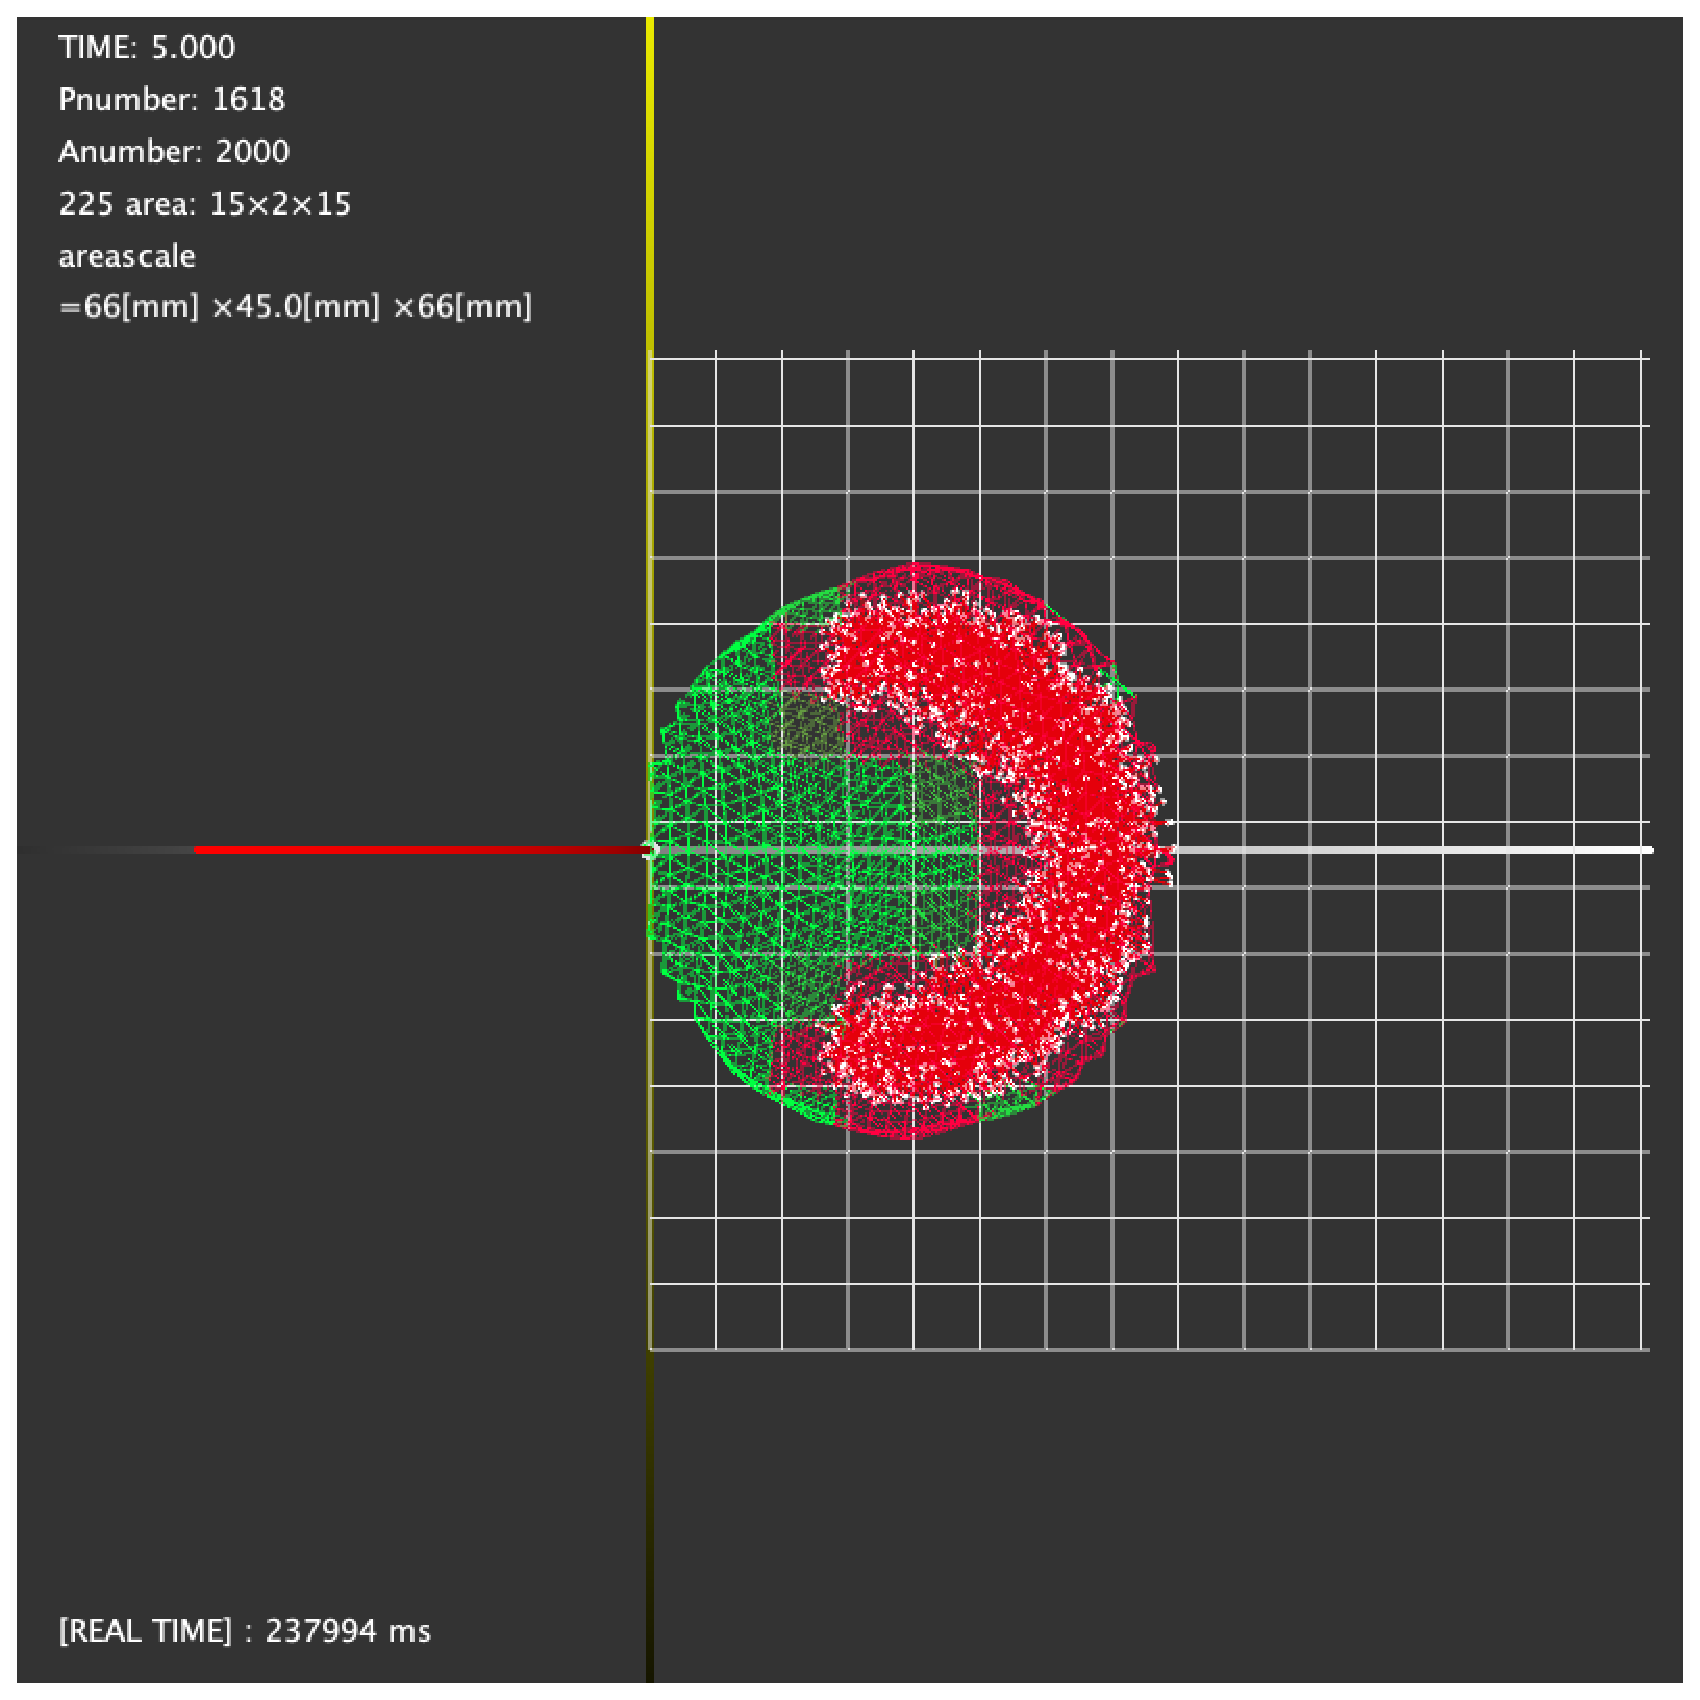
\includegraphics[width=5cm]{50_nro.eps} 
  \end{tabular}
 }%
 \subfloat[]{%
  \begin{tabular}{c}
   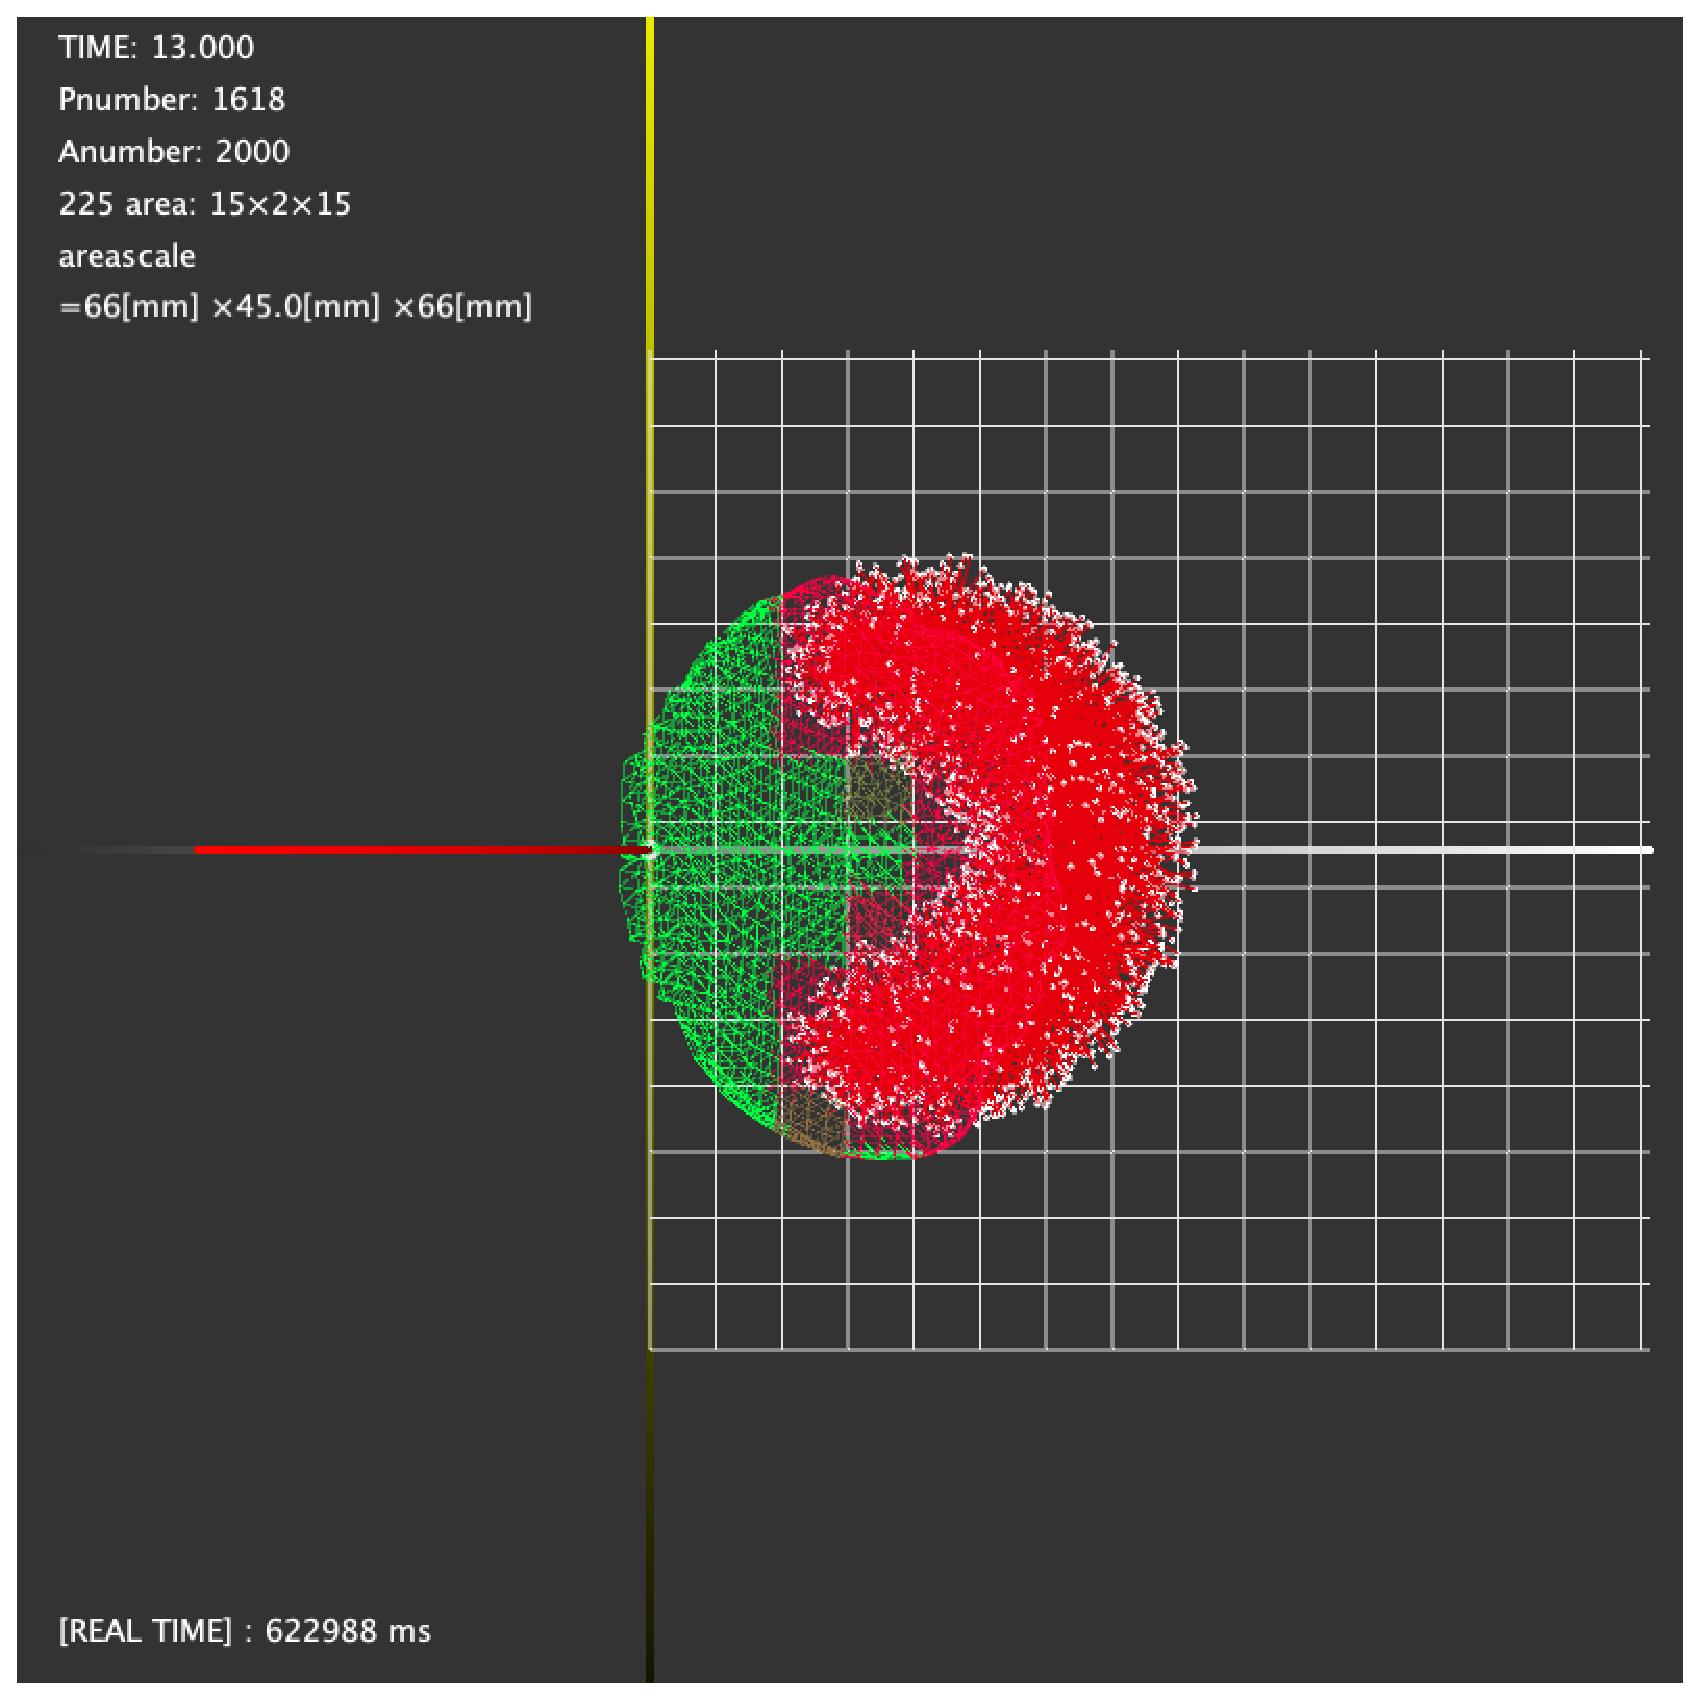
\includegraphics[width=5cm]{90_nro.eps} 
  \end{tabular}
 }%
 \caption{Simulation results without the orientation effect on the actin molecules by the ARF. The subfigures show the results at different timings as in Fig. \ref{fig:res0}.}
 \label{fig:res4}
\end{figure}

\begin{figure}[tbp]
 \subfloat[]{%
  \begin{tabular}{c}
   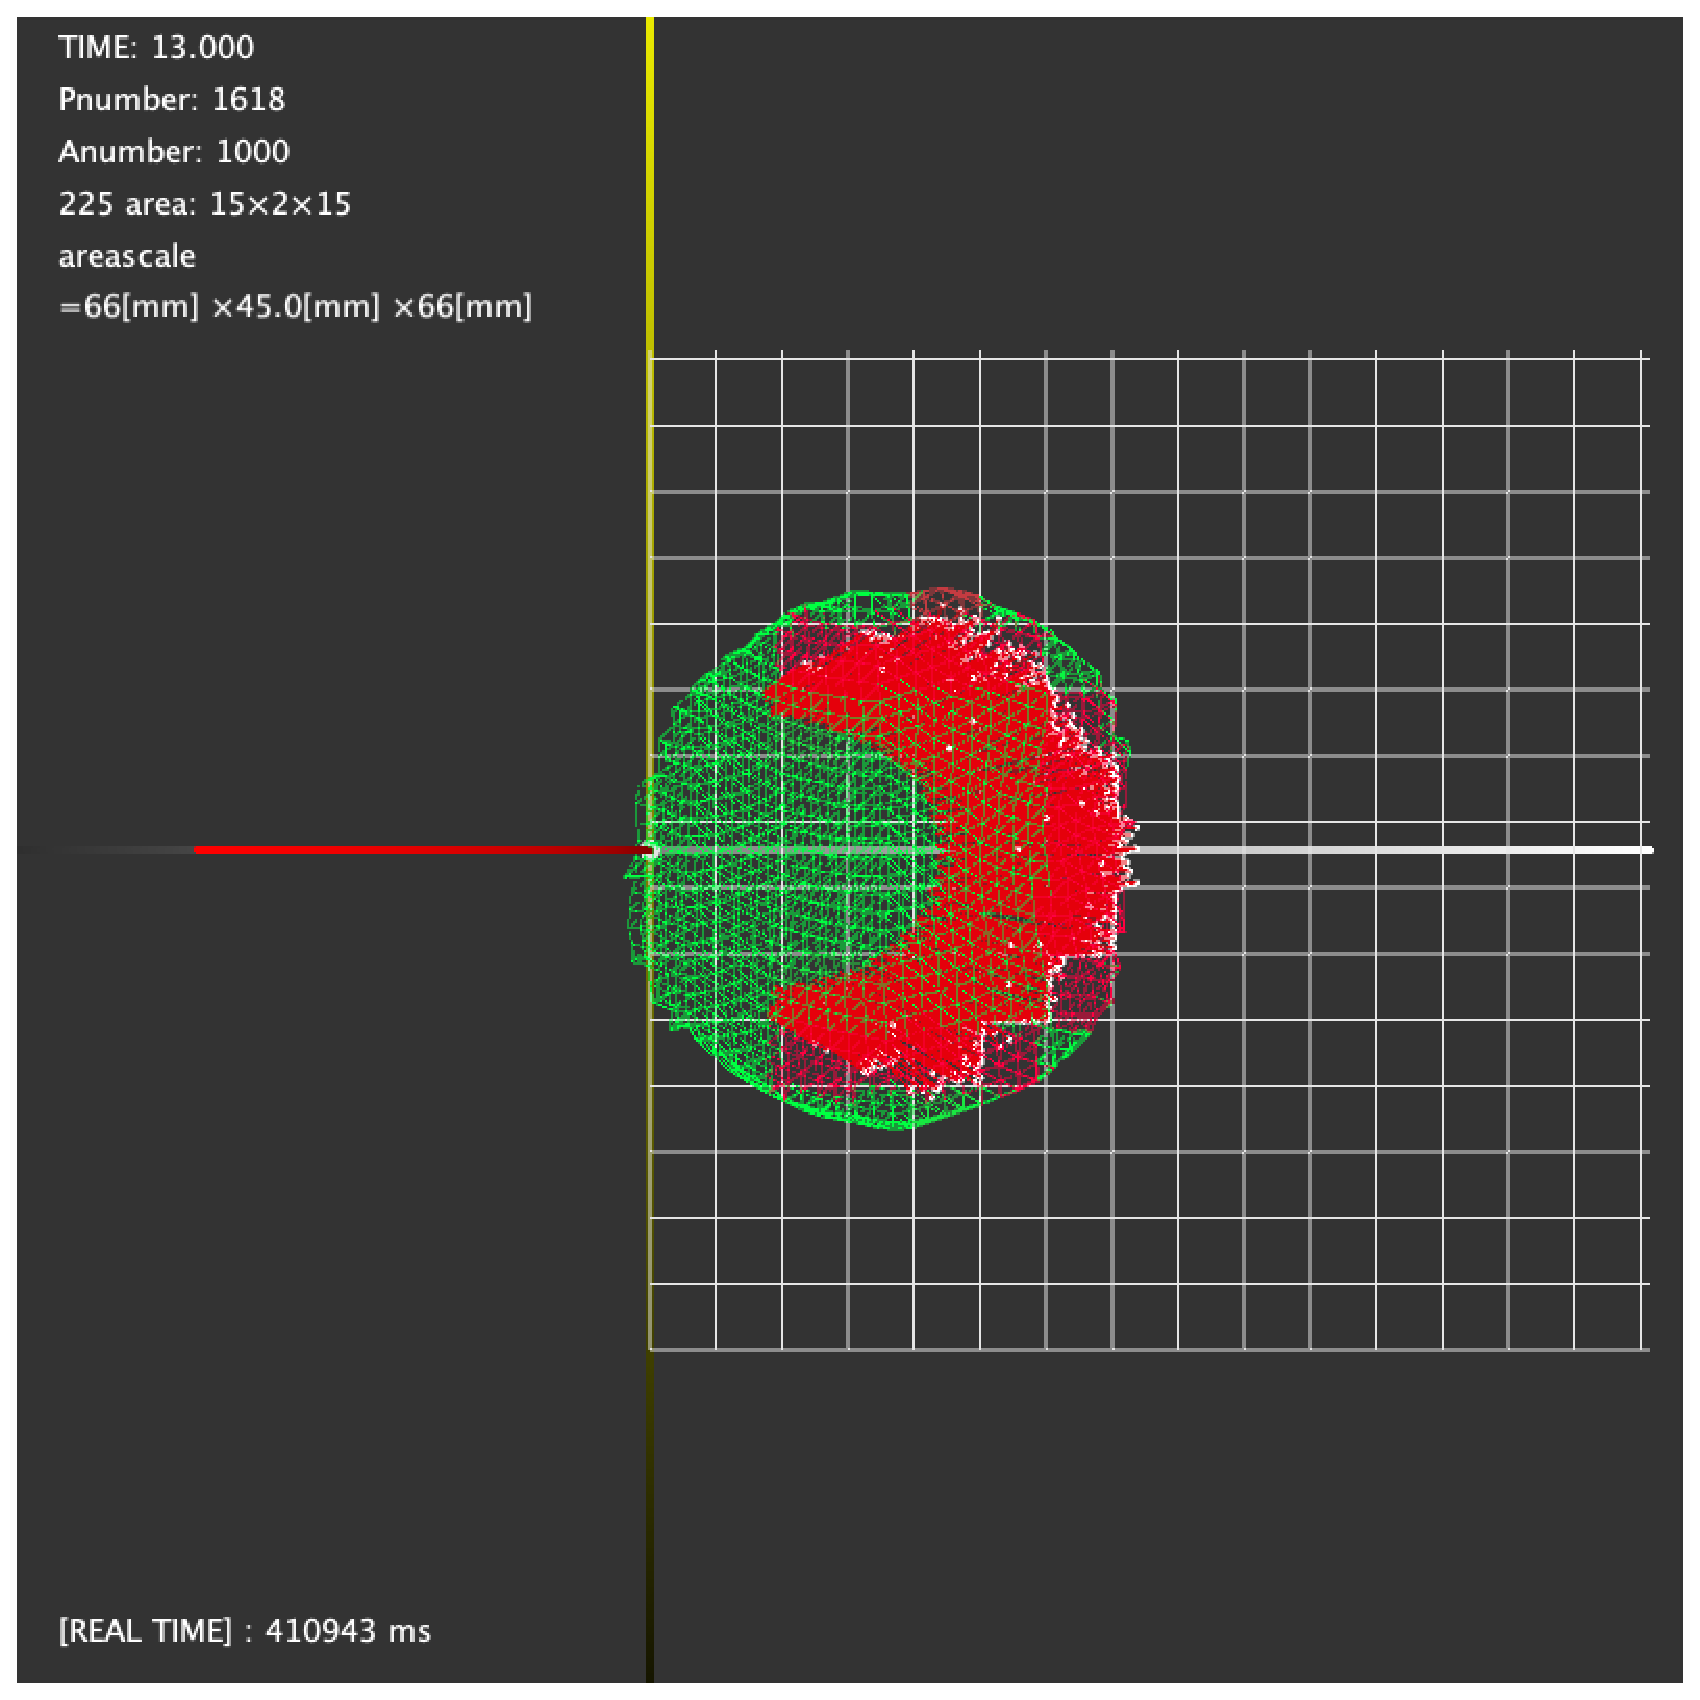
\includegraphics[width=5cm]{13_arf.eps} 
  \end{tabular}
 }%
 \subfloat[]{%
  \begin{tabular}{c}
   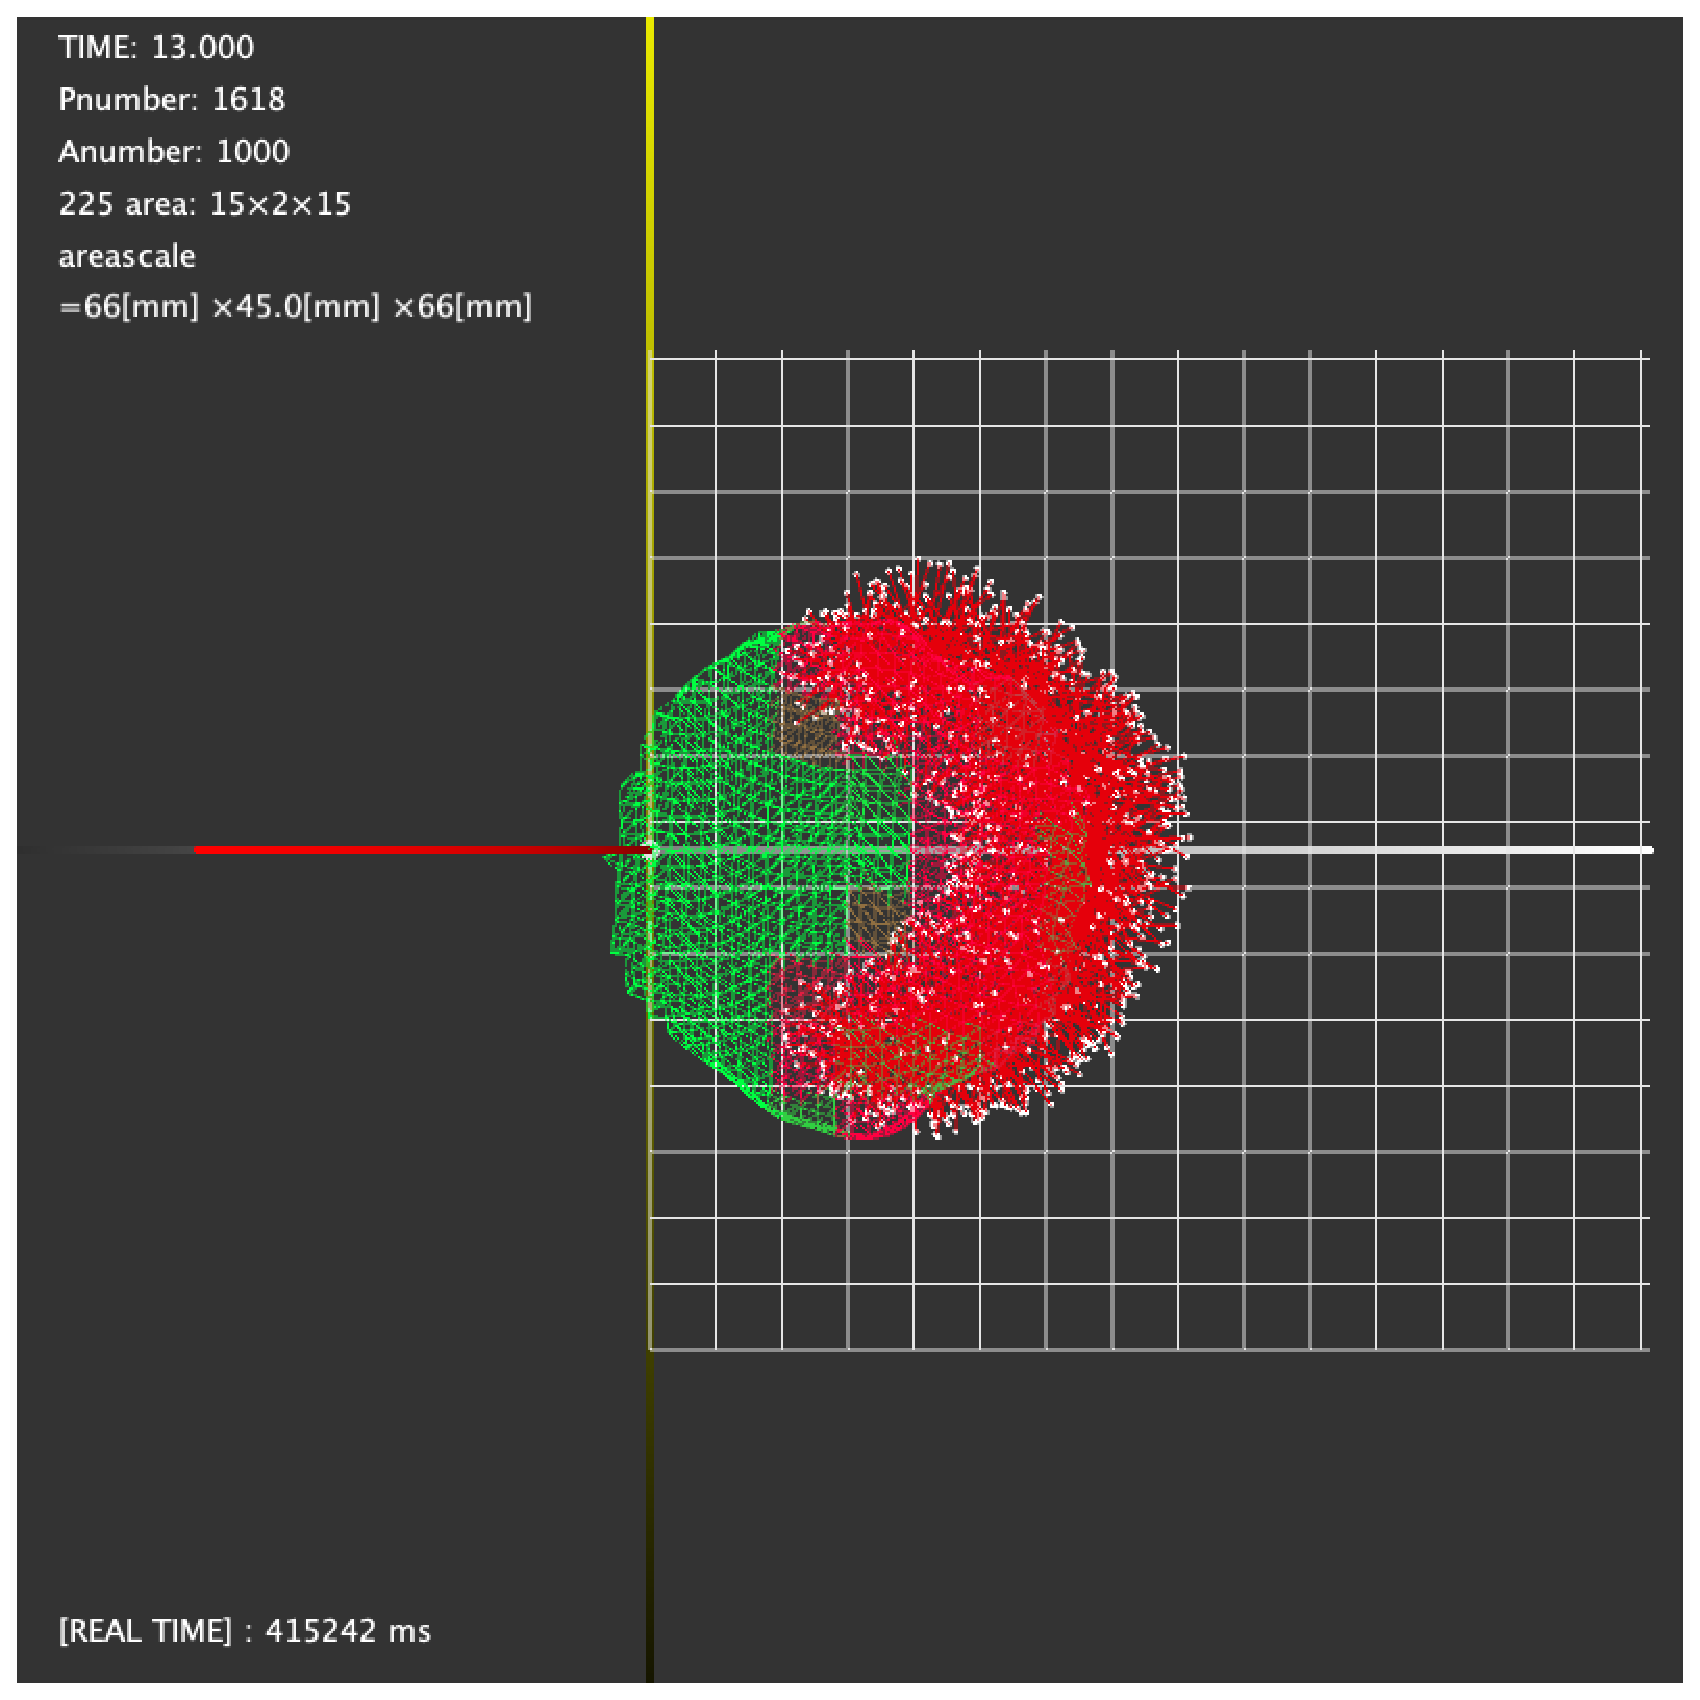
\includegraphics[width=5cm]{13_nro.eps} 
  \end{tabular}
 }%
 \caption{Simulation results at $t=13$~[s]. (a) and (b) are the results when orientation effect on actin molecules was considerd and ignored, respectively.}
 \label{fig:res5}
\end{figure}
%大元の結果
Fig. \ref{fig:res0} shows the simulation result when two reference points of the ARF is prepared (eq. (\ref{eq:arf})) and the effect of the ARF is independent of the distance (w=1 in eq. (\ref{eq:arf})).
In this case, the actin molecules aggregated in a half-moon shape and the shape was kept for a long time even after the time shown in Fig.\ref{fig:res0}~(c).

%距離依存との比較
Fig. \ref{fig:res1} shows the results under the same condition as Fig. \ref{fig:res0} except that distance-dependent ARF was assumed (w=2 in eq. (\ref{eq:arf})).
Since actin molecules close to the SF were strongly pulled back by the ARF in the case, the region of actin molecule were elongated toward the SF and the membrane received repulsive force from actin molecules only on the front end of the cell.
When the repulsive force converges at specific region of the membrane, the cell membrane was broken.
Therefore, in order for the actin molecule to aggregate in a crescent moon shape, it is necessary to polymerize in a radial pattern.

%1点集中との比較
Fig. \ref{fig:res2} shows simulation results when one reference point of the ARF was prepared (eq. (\ref{eq:arf1})).
The actin molecules migrated toward the center of the cell and the half-moon shape was not achieved.
When the actin molecules aggregate in a circular shape, the direction of movement of the cell was not determined because they push the entire cell membrane.
These results suggest that the retraction of actin molecules by the ARF toward not a point but the SF is an important phenomenon to make the cell shape a half-moon.

%ARFの有無
Fig. \ref{fig:res3} shows the simulation results when the retraction of actin molecules by the ARF was ignored.
Actin molecules were elongated by  polymerization toward  random directions.
This result shows that the retraction by the ARF is important to keep specific cell size against actin polymerization.

%回転なし
Fig. \ref{fig:res4} showed the simulation result when ignoring the orientation effect by the ARF.
%fig4.5cの説明
The actin molecules aggregated into a V-shape and broke the cell membrane.
Paying attention to the white dots which is barbed-end, when compared with Fig.~\ref{fig:res0}, no alignment of the actin molecules was observed.
The shapes in Fig.~\ref{fig:res4} and Fig.~\ref{fig:res0} are similar, but since the barbed-end of the actin molecule is oriented in all directions in Fig.~\ref{fig:res4}, the shape because differ after sufficient time~(Fig.~\ref{fig:res5}). 
Without an orientation effect, the actin molecule region spreads without changing its shape.
In contrast, in the presence of an orientation effect, the region of the actin molecule is within the cell membrane over time.
This result suggests that the effect of aligning the polymerization direction prevents the expansion of the actin molecule region.

\subsection{Effect of Initial Distribution of Actin Molecules}
\begin{figure}[tbp]
 \subfloat[]{%
  \begin{tabular}{c}
   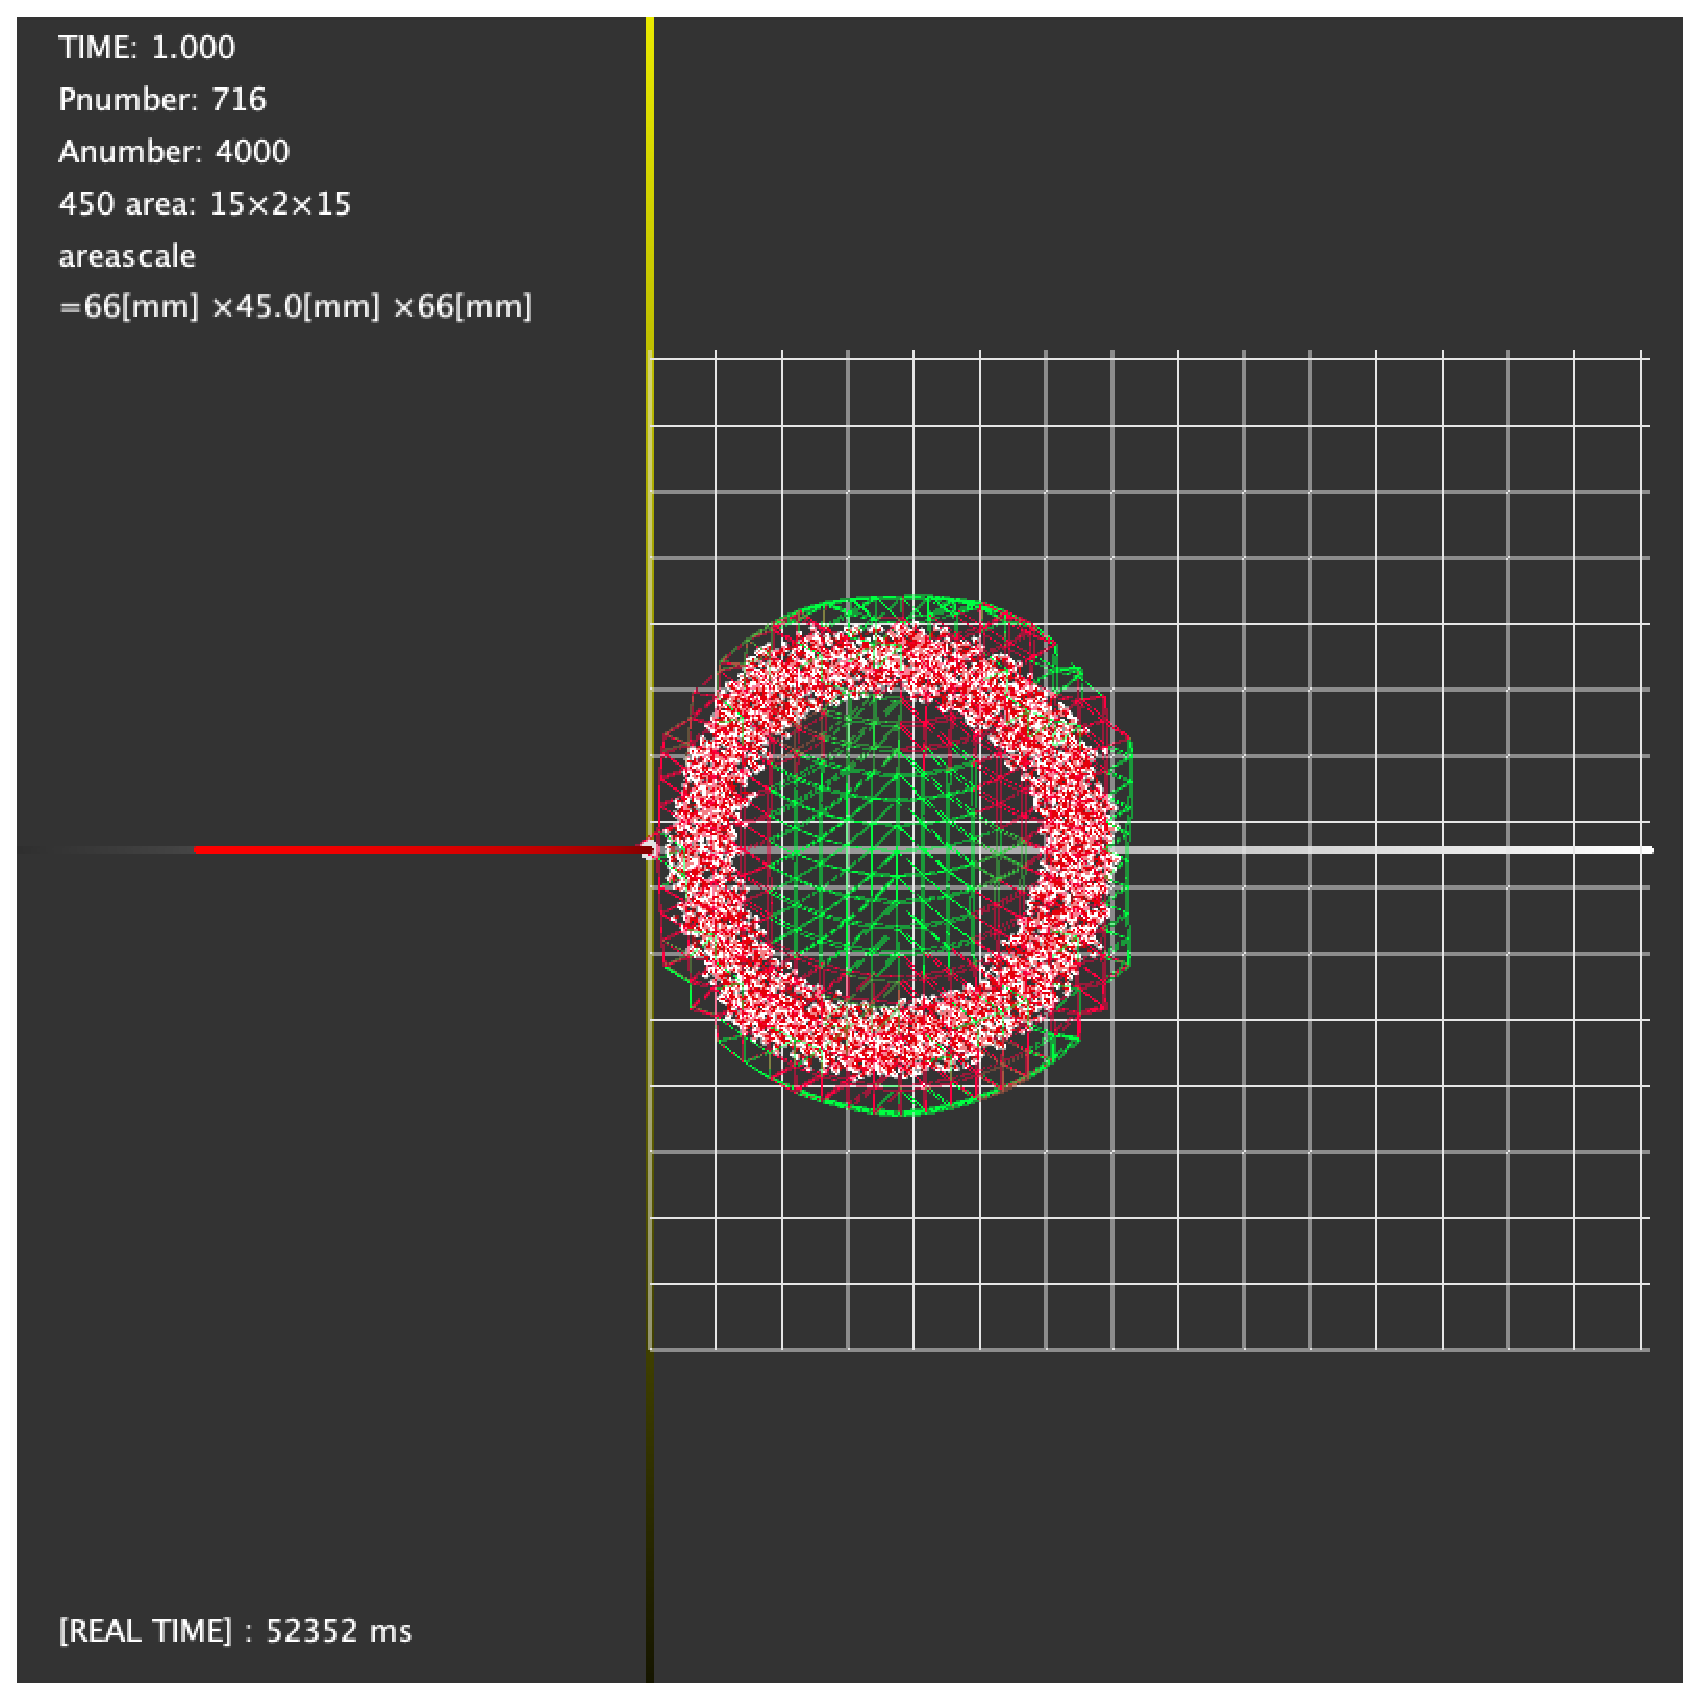
\includegraphics[width=5cm]{10_ci.eps} 
  \end{tabular}
 }%
 \subfloat[]{%
  \begin{tabular}{c}
   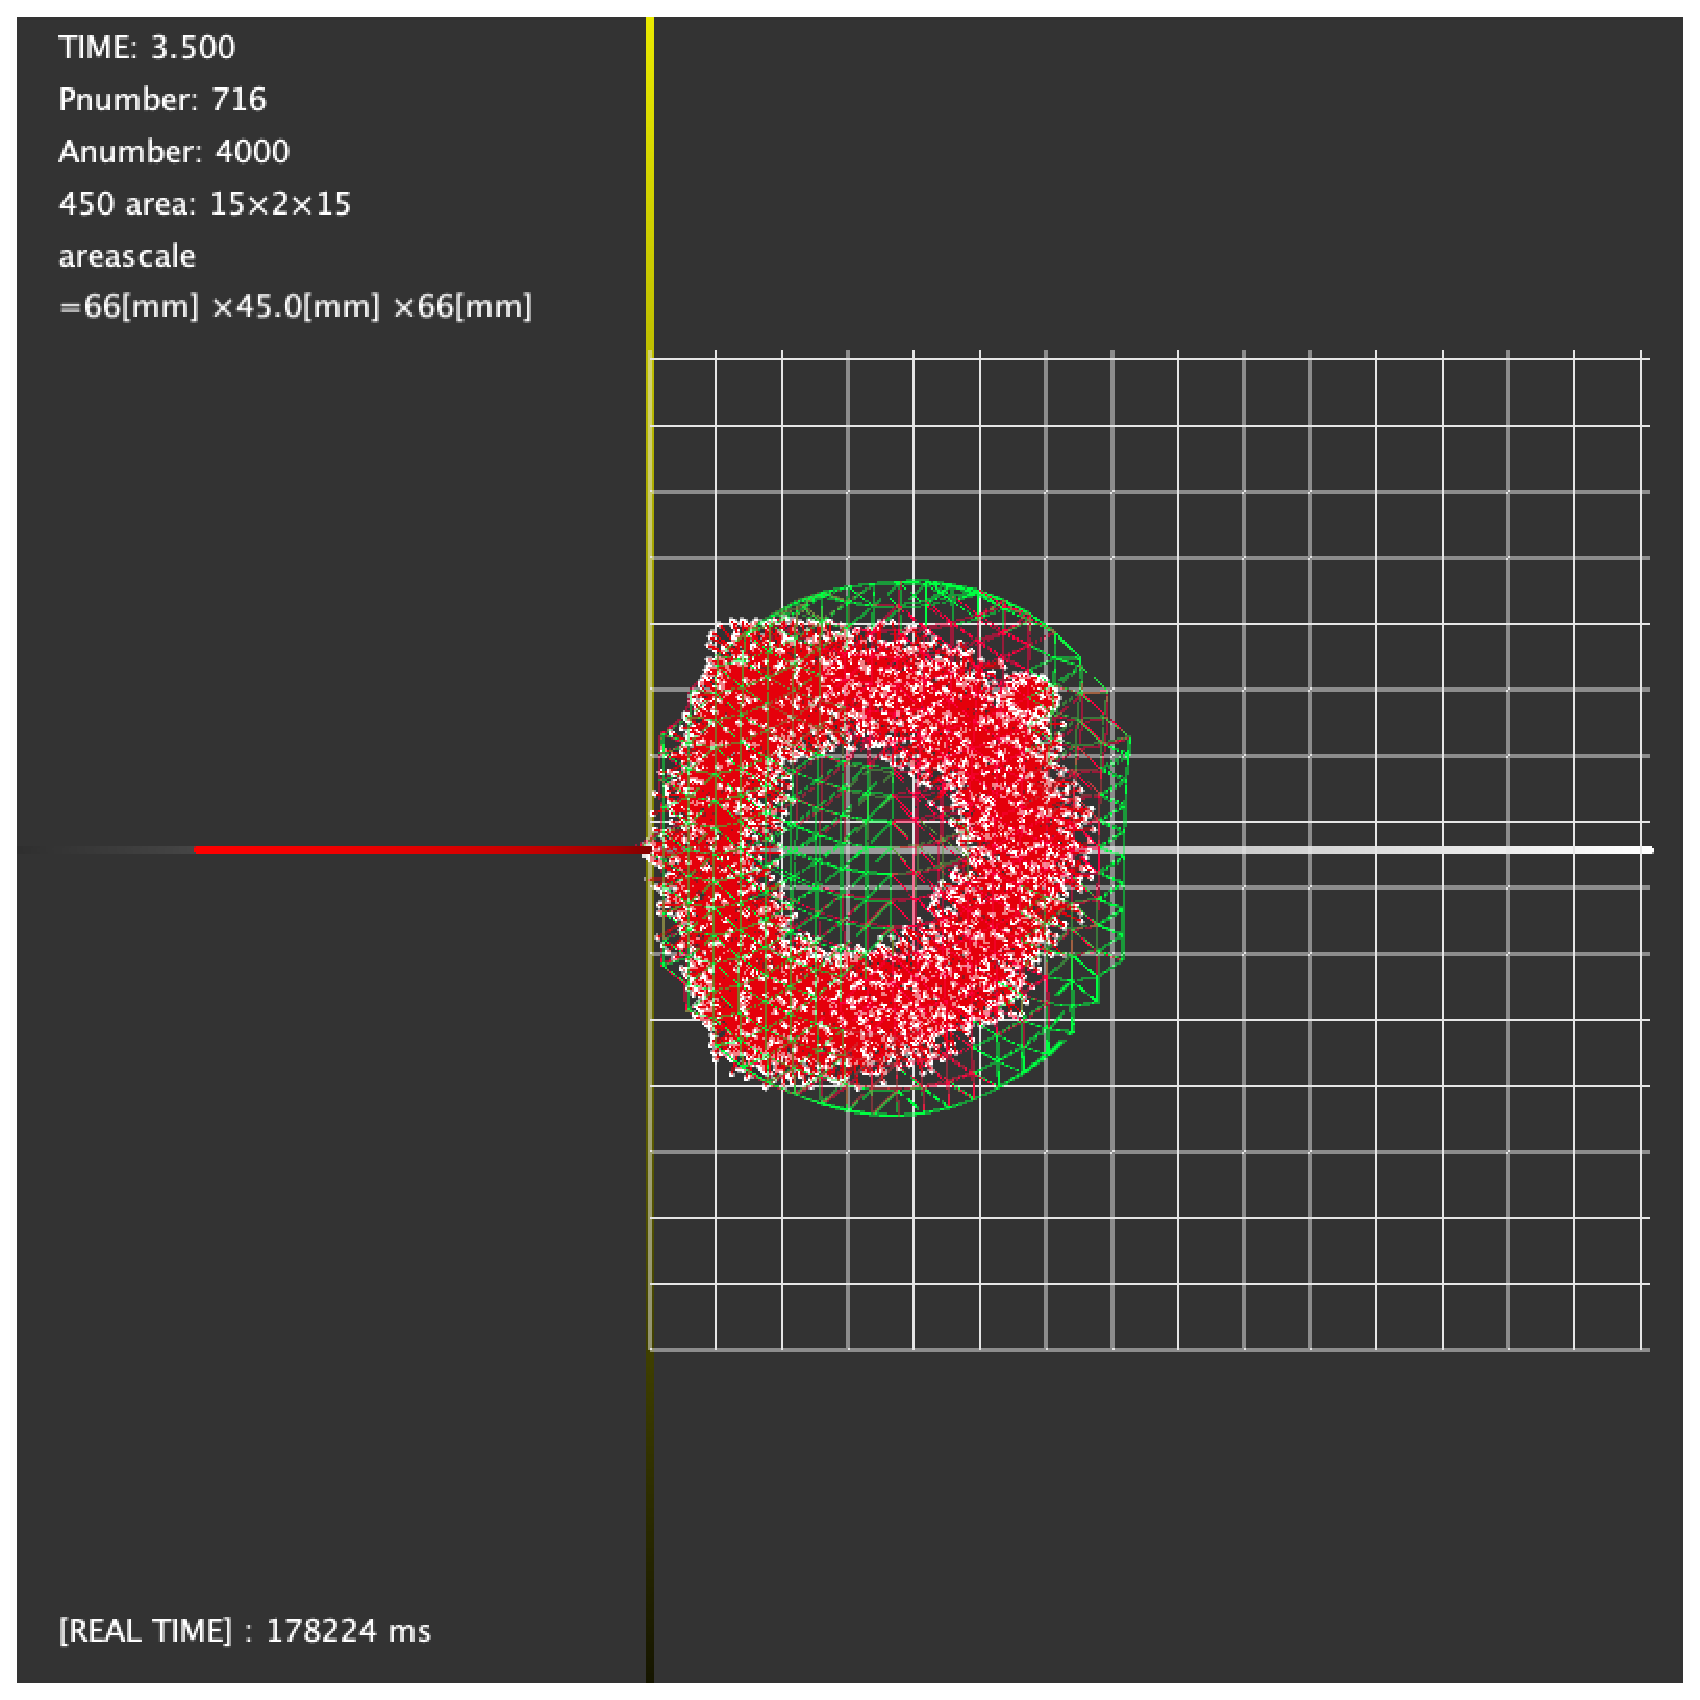
\includegraphics[width=5cm]{50_ci.eps} 
  \end{tabular}
 }%
 \subfloat[]{%
  \begin{tabular}{c}
   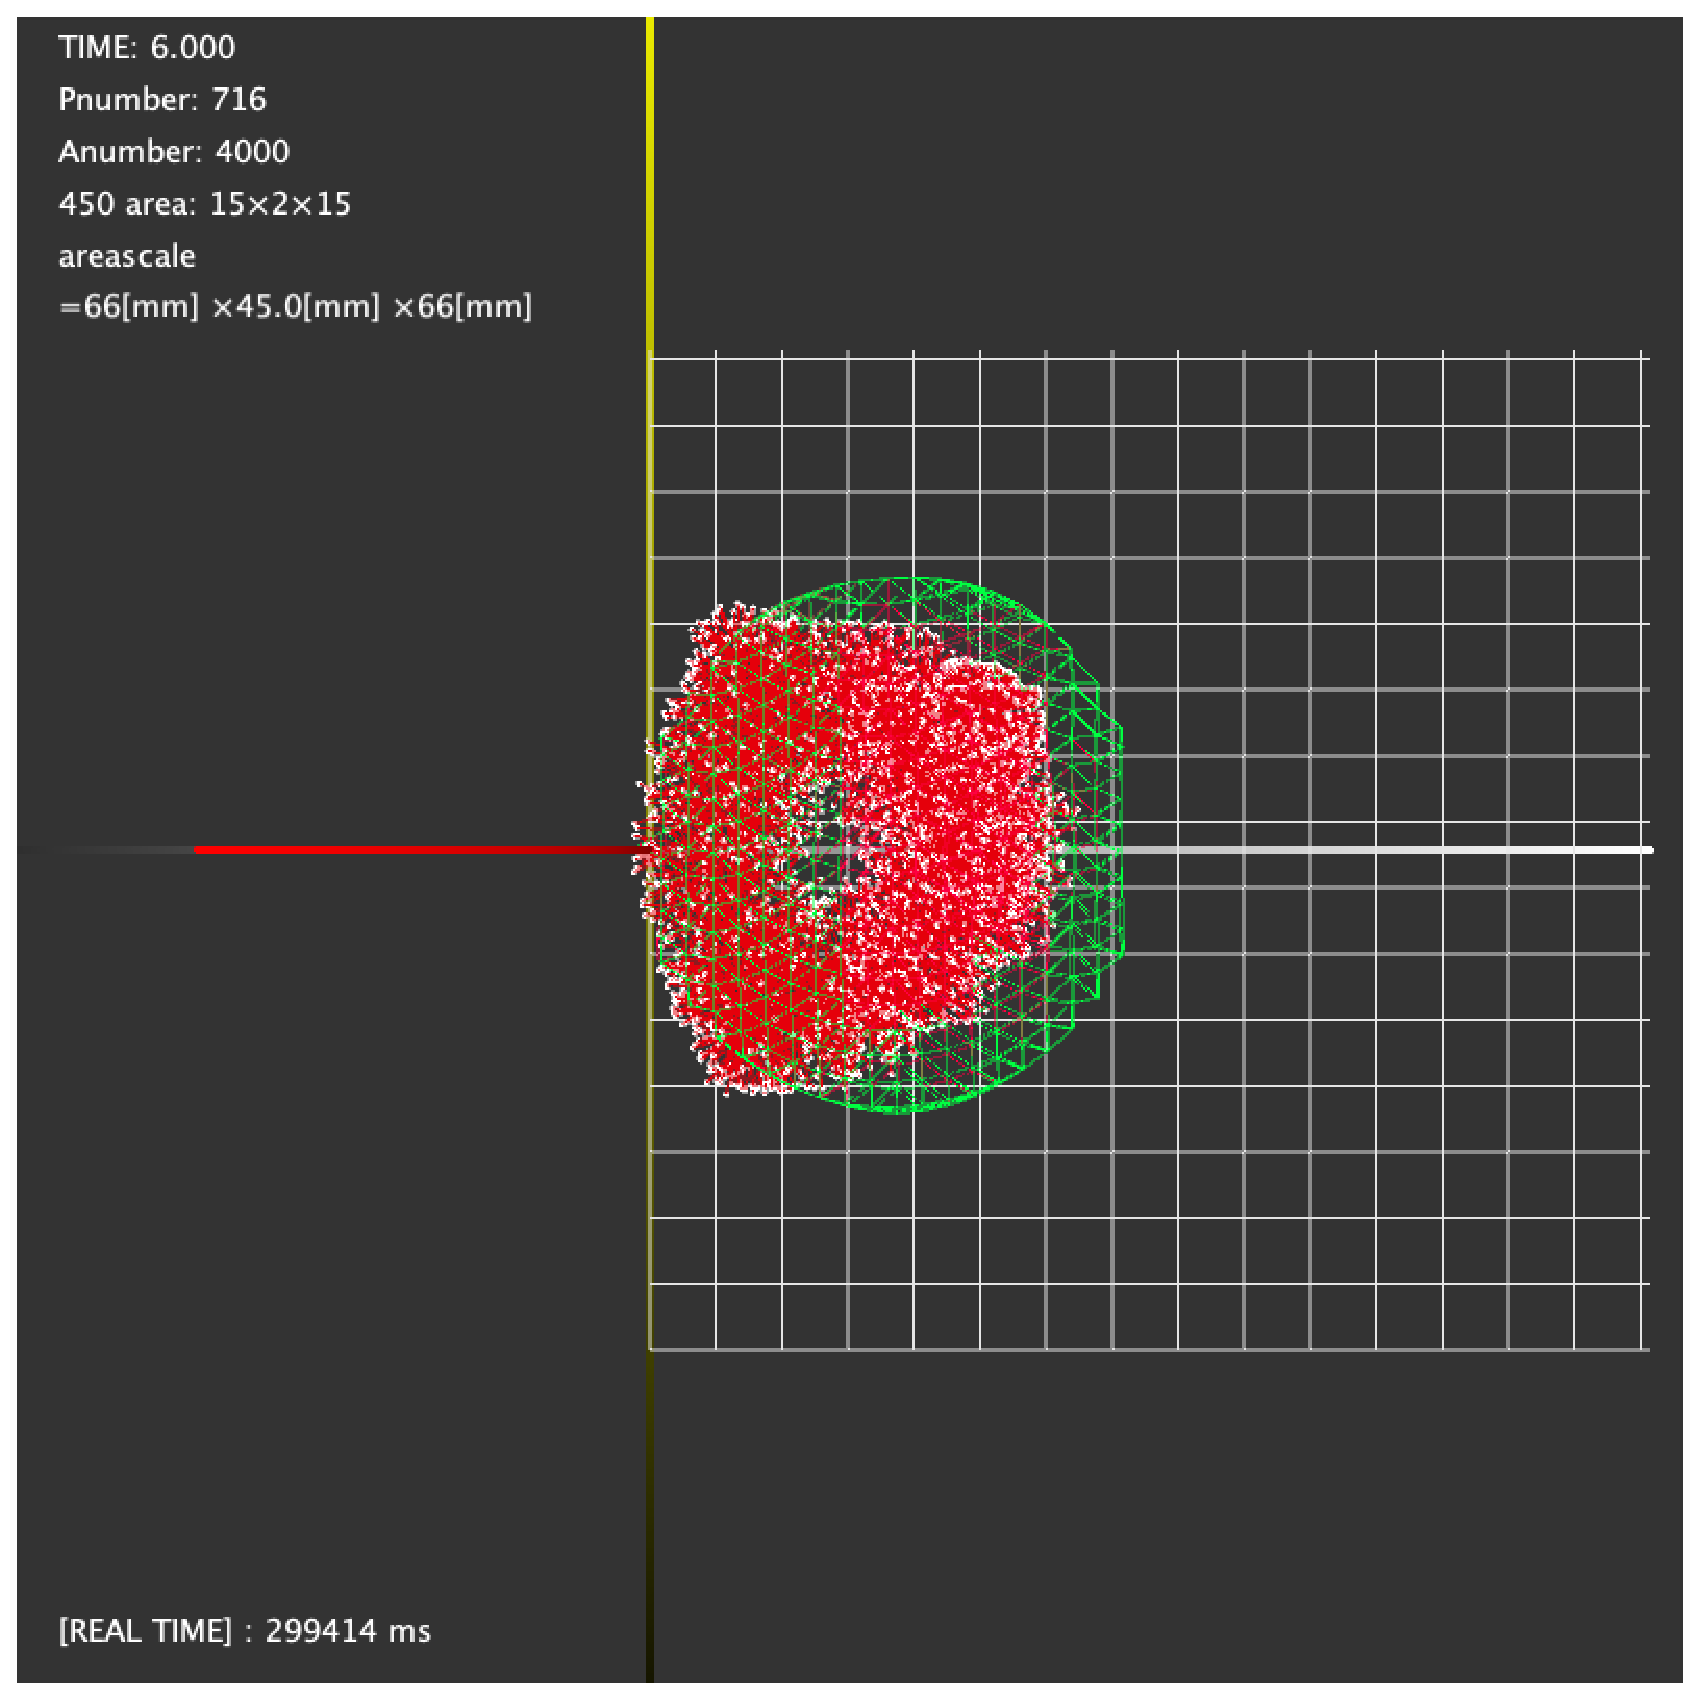
\includegraphics[width=5cm]{90_ci.eps} 
  \end{tabular}
 }%
 \caption{Simulation results when actin molecules were distributed in a circular region as an initial condition. The subfigures show the results at different timings as in Fig. \ref{fig:res0}.}
 \label{fig:res6}
\end{figure}

In the simulation experiments in the previous section, the actin molecules were randomly distributed in a U-shaped region as an initial condition.
Fig. \ref{fig:res5} shows the simulation results when actin molecules were distributed in a donut shape.
The other simulation conditions were the same as those in Fig. \ref{fig:res0}.
The actin molecule did not aggregate in a half-moon shape but around the SF.
This is because around the SF affects the actin molecules but does not remove them in the rear part of the cell.
From the results in Fig.\ref{fig:res0} and Fig.\ref{fig:res5}, it clear that actin molecules aggregated from a donut shape to a U-shape form and then agglomerated in a half-moon shaped form.In keratocytes, the number of actin molecules decreases at the rear part of the cell when migration starts \cite{ridley2003cell}.
Hence, such a break of uniform distribution of the actin is a key to the formation of the half-moon shape.  

\subsection{Discussion on the Relationship between the AP and the ARF}
%結果をまとめる
All conditions under which the actin molecules aggregated in a half-moon shape were related to the existence of the ARF.
The AP in this simulation was only imposed to the condition that the actin molecule extends in a specific direction and extends more into a high density of region actin molecules.
However, Fig.~\ref{fig:res3} showed that actin molecules do not aggregate in a half-moon shape simply by polymerization.
The simulation results showed that the retraction and orientation of actin molecules by the ARF contributes to the formation of the half-moon shape and the regulation of the cell size, respectively.

%なぜ半月状を形成できたのか?
%配向効果、基準点がSF、U字型、一様に引っ張る
%先に牽引効果
When the AP in a specific area is particularly active (Fig.~\ref{fig:res1}), they did not form in a half-moon shape.
If all the actin molecules were not pulled uniformly, it was impossible to form a half-moon shaped circular arc as shown in Fig. 
\ref{fig:res1}.
The effect of pulling actin molecules with distance independence contributes to the shape of the aggregation region of the actin molecule as well as its keeping.

%つぎに配向効果
Even when there is no orientation effect of the ARF, actin molecules aggregated in a half-moon shape if there is a retraction effect(Fig.\ref{fig:res4}).
However, in the absence of orientation effect, actin molecules are polymerized in all directions and the region of actin molecules continues to expand.
The change in the direction of polymerization of actin molecule by the ARF results in the alignment of the barbed-end around the membrane.
That is, the orientation effect is an effect of deforming the shape of aggregation by changing the extending direction of actin molecules.
As the polymerization direction of actin molecule changes, the actin molecule density in each region also changes.
As the actin molecule density in each region changes, the position of the region where the actin molecule disappears is changed everywhere.
As the area where actin molecule disappears increases, it becomes difficult to expand the aggregation size of actin molecule.
It is speculated that ARF controls AP by such a mechanism.

\chapter{Conclusion}
\section{Conclusion}
%本研究では何をして,どのような結果について,目的に対応するポイントを簡潔にまとめる。(どういうシミュレーションをして,どういう結果になったか。どのような発見があったか)
The purpose of this research was to clarify the mechanism that forms a half-moon shape by physical simulation experiments considering intracellular mechanism.
In the computer simulation of this study, the cell membrane was modeled by a network of simple particles interacting with each other and placed on a cylindrical surface as an initial condition.
Each particle of the membrane was assumed to receive elastic force from neighboring particles and repulsive force from actin molecules.
Actin molecules were modeled by a simple rod, and polymerization and depolymerization were expressed by stochastic elongation of one end of the rod and contraction of the other end, respectively.
As an initial condition, actin molecules have no length and were randomly distributed in a U-shaped region, and the direction of the The AP of each molecule was randomly determined.
As an effect of the ARF, actin molecules were assumed to move toward the SF stochastically and oriented in the direction in which actin molecule is pulled.
As a result, the actin molecules aggregated in a half-moon shape due to the tow effect of the ARF, and a half-moon shape was kept by the orientation effect.
These results show that ARF plays an important role in the formation of a half-moon shape.

\section{Future Works}
%この研究の大きな目的に到達するために何をしていくべきかがわかるような書き方が必要。手段を列挙するのではなく,目的を達成するために何を今後する必要があるか,その必要性を感じさせる書き方をする。
%本実験における問題点と解決法を先に説明。その後,大きな目的に向かうための今後の課題の説明。
If the positions of actin molecules is do not change by the retraction of the ARF, the cell does not move.
More detailed conditions need to be added to the ARF condition.
For example, if the condition that the pulling intensity of ARF changes over time is added, the shape is maintained without being unnecessarily pulled after the actin molecule aggregates in a half-moon shape.


There was a problem with the simulation of cell membranes receiving repulsive force from actin molecules.
Even when the front end of the cell receives the repulsive force from the actin molecules, the deformation did not propagate to the rear of the cell.
There is a possibility that there is a bug in the bond between the membrane molecules.
If we can introduce temporal changes to the conditions related to the ARF and model cell membranes without bugs, we can elucidate the mechanism by which cell membranes form a half-moon shape.

\chapter*{Acknowledgements}
I would like to thank Prof. Nishii whose enormous support and insightful comments were invaluable during the course of my study. I also owe a very important debt to Prof. Urakami, Prof. Iwadate and the members of the laboratory whose comments made an enormous contribution to my work. 

\addcontentsline{toc}{chapter}{Acknowledgements}
\bibliography{bibtexfile.bib}
\bibliographystyle{junsrt}

\addcontentsline{toc}{chapter}{\bibname}
\end{document}
